\documentclass{article}\usepackage[]{graphicx}\usepackage[]{color}
% maxwidth is the original width if it is less than linewidth
% otherwise use linewidth (to make sure the graphics do not exceed the margin)
\makeatletter
\def\maxwidth{ %
  \ifdim\Gin@nat@width>\linewidth
    \linewidth
  \else
    \Gin@nat@width
  \fi
}
\makeatother

\definecolor{fgcolor}{rgb}{0.345, 0.345, 0.345}
\makeatletter
\@ifundefined{AddToHook}{}{\AddToHook{package/xcolor/after}{\definecolor{fgcolor}{rgb}{0.345, 0.345, 0.345}}}
\makeatother
\newcommand{\hlnum}[1]{\textcolor[rgb]{0.686,0.059,0.569}{#1}}%
\newcommand{\hlstr}[1]{\textcolor[rgb]{0.192,0.494,0.8}{#1}}%
\newcommand{\hlcom}[1]{\textcolor[rgb]{0.678,0.584,0.686}{\textit{#1}}}%
\newcommand{\hlopt}[1]{\textcolor[rgb]{0,0,0}{#1}}%
\newcommand{\hlstd}[1]{\textcolor[rgb]{0.345,0.345,0.345}{#1}}%
\newcommand{\hlkwa}[1]{\textcolor[rgb]{0.161,0.373,0.58}{\textbf{#1}}}%
\newcommand{\hlkwb}[1]{\textcolor[rgb]{0.69,0.353,0.396}{#1}}%
\newcommand{\hlkwc}[1]{\textcolor[rgb]{0.333,0.667,0.333}{#1}}%
\newcommand{\hlkwd}[1]{\textcolor[rgb]{0.737,0.353,0.396}{\textbf{#1}}}%
\let\hlipl\hlkwb

\usepackage{framed}
\makeatletter
\newenvironment{kframe}{%
 \def\at@end@of@kframe{}%
 \ifinner\ifhmode%
  \def\at@end@of@kframe{\end{minipage}}%
  \begin{minipage}{\columnwidth}%
 \fi\fi%
 \def\FrameCommand##1{\hskip\@totalleftmargin \hskip-\fboxsep
 \colorbox{shadecolor}{##1}\hskip-\fboxsep
     % There is no \\@totalrightmargin, so:
     \hskip-\linewidth \hskip-\@totalleftmargin \hskip\columnwidth}%
 \MakeFramed {\advance\hsize-\width
   \@totalleftmargin\z@ \linewidth\hsize
   \@setminipage}}%
 {\par\unskip\endMakeFramed%
 \at@end@of@kframe}
\makeatother

\definecolor{shadecolor}{rgb}{.97, .97, .97}
\definecolor{messagecolor}{rgb}{0, 0, 0}
\definecolor{warningcolor}{rgb}{1, 0, 1}
\definecolor{errorcolor}{rgb}{1, 0, 0}
\makeatletter
\@ifundefined{AddToHook}{}{\AddToHook{package/xcolor/after}{
\definecolor{shadecolor}{rgb}{.97, .97, .97}
\definecolor{messagecolor}{rgb}{0, 0, 0}
\definecolor{warningcolor}{rgb}{1, 0, 1}
\definecolor{errorcolor}{rgb}{1, 0, 0}
}}
\makeatother
\newenvironment{knitrout}{}{} % an empty environment to be redefined in TeX

\usepackage{alltt}
\usepackage{hyperref}
%\usepackage{expl3}
%\usepackage{l3regex}
%\usepackage[version=4]{mhchem}
% \usepackage{animate}


\begin{knitrout}
\definecolor{shadecolor}{rgb}{0.969, 0.969, 0.969}\color{fgcolor}\begin{kframe}


{\ttfamily\noindent\bfseries\color{errorcolor}{\#\# Error: <text>:6:0: unexpected end of input\\\#\# 4: png\_private = \\\#\# 5: gif\_public = \\\#\# \ \ \textasciicircum{}}}\end{kframe}
\end{knitrout}





\begin{knitrout}
\definecolor{shadecolor}{rgb}{0.969, 0.969, 0.969}\color{fgcolor}\begin{kframe}
\begin{alltt}
\hlstd{get_locationid} \hlkwb{<-} \hlkwa{function}\hlstd{(}\hlkwc{FIPS}\hlstd{)\{}
   \hlstd{fips} \hlkwb{=} \hlkwd{ncdc_locs}\hlstd{(}\hlkwc{locationcategoryid}\hlstd{=}\hlstr{'ST'}\hlstd{,} \hlkwc{limit}\hlstd{=}\hlnum{55}\hlstd{)}
   \hlstd{temp} \hlkwb{<-} \hlkwd{data.frame}\hlstd{(}\hlkwc{State} \hlstd{= fips}\hlopt{$}\hlstd{data}\hlopt{$}\hlstd{name[FIPS],}
             \hlkwc{id} \hlstd{= fips}\hlopt{$}\hlstd{data}\hlopt{$}\hlstd{id[FIPS])}
   \hlstd{temp}\hlopt{$}\hlstd{id} \hlkwb{<-} \hlkwd{as.character}\hlstd{(temp}\hlopt{$}\hlstd{id)}
   \hlstd{temp}\hlopt{$}\hlstd{State} \hlkwb{<-} \hlkwd{as.character}\hlstd{(temp}\hlopt{$}\hlstd{State)}
   \hlkwd{return}\hlstd{(temp)}
\hlstd{\}}
\end{alltt}
\end{kframe}
\end{knitrout}

\begin{knitrout}
\definecolor{shadecolor}{rgb}{0.969, 0.969, 0.969}\color{fgcolor}\begin{kframe}
\begin{verbatim}
## 'data.frame':	1 obs. of  2 variables:
##  $ State: chr "Alabama"
##  $ id   : chr "FIPS:01"
\end{verbatim}
\end{kframe}
\end{knitrout}

\title{Weather Station Records and Communicating Climate Change--Alabama}
%\subtitle{test}
\author{Marc Los Huertos}
\IfFileExists{upquote.sty}{\usepackage{upquote}}{}
\begin{document}

\maketitle

\tableofcontents

\section{Evaluating Terrestrial Meteorological Data}

\subsection{Selected History of Climate Science}

Geologists have known the climate has been changing over the Earth's history. But what causes these changes has been a major research area for over 100 years. There are numerous drivers that contribute to changing climates -- including the arrangement of the continents on the planet, the distance to the sun, energy generated by the sun, volanic activity, and the composition of the Earth's atmosphere. 

It's the last one that we'll spend time because the Earth's temperature are changing pretty dramatically over the last 100 years and the cause is no mystery -- the human activity that has released carbon dioxide (CO$_2$) into the atmosphere. The two main sources of CO$_2$ is from land use change, e.g. deforestration, and the burning of fossil fuels, e.g. coal, oil, and natural gas. 

The first to propose the role of CO$_2$ on the Earth's atmosphere was a Swedish scientist Svante Arrhenius, who figured out that CO$_2$ absorbs infarred light. Moreover, he deduced that the Earth's temperature was actually warmer than it might otherwise be if CO$_2$ was not part of the Earth's atmoshere. 

\subsection{Why Look at Individual Stations?}

I don't think there is a single, perfect way to analyze and communicate climate change. But the beauty of the network of stations in the USA and around the world is that these stations record weather as expecienced by local people. And while indiviudual stations may not represent the overall regional and global patterns well, this give us a mechanism to connect local experiences to regional or global processes. 

Of course, some may fixate on the local pattern and remain unconvinced of the larger context and for those folks, there may be better ways to communicated climate data. 

However, I would be remiss in failing to mention that some may fixate on local patterns and use these patterns to ignore or to dimiss the patterns in other regions. 

Finally, the impacts of climate change are highly specific to the region in question. Thus, once someone understands the impacts on climate change in their region, they my not be able to appreciate how differnet the climate impacts might affect other peoples, who maybe more vulneratble, around the globe. 

Thus, with these weaknessed in mind, I will pursue this project with an eye to address these other issues at later stages.

\subsection{Approach}

\subsubsection{NOAA Data Records}

The US National Oceanic and Atmospheric Adminstration (NOAA) maintains several sources of digital weather data from the USA and beyond. These data have been collected from stations around the country to support a wide range of human activities that include farming, aviation, shipping, and even armed conflict. 

At various times, these records have been used to evaluate long-term climate change with varying success. Without a doubt, these data are not perfect, but they remain that foundation of an effective adn professionally maintained environmental monitoring program that engenders integrity, even when facing budget cuts. 

I will use these data to select for a station with a long record for each state in the USA. Future projects might evaluate the record for stations around the world, but we will see about that. 

%ftp://ftp.ncdc.noaa.gov/pub/data/ghcn/v3/

\subsubsection{rNOAA Package and R}

R is an open source programming environment that has become one of the most popular tools for statiticians and data scientists. Capitalizing on the open source framework, a wide range of libraries or packages have been developed to faciliate data processing, analysis, and graphical displays. On such package is rNOAA developed to collect and display climate records stored on NOAA servers.

Using the package requires the use of a key. To maintain the integrity of the key, it's best to avoid posting the key in a public repository and to encryp the key to ensure it's not abused. 

\subsection{Selecting Weather Records by State}

There are numerous ways to analyze temperature records, where stations can be analyzed individually or records could be sampled and analyzed in spatially in grids. Each of these are valid approaches depending on the question to be addressed. 

In this case the question is ``Based on the longest state meterological record, is there a temperature trend?"

\subsubsection{Identify List of State IDs (FIPS)}

Using the rNOAA library in R, we can queary NOAA's database to identify station codes (FIPS) by state. With the states and some territories, there are 55 FIPS for US weather stations. 

rNOAA has a simple function to list for each of the states and the weather stations in each. I use ncdc\_locs() functions to select each state and ncdc\_station() to obtain the station ids with the longest records. 

\begin{knitrout}
\definecolor{shadecolor}{rgb}{0.969, 0.969, 0.969}\color{fgcolor}\begin{kframe}
\begin{alltt}
\hlcom{# List of States (alpha beta)}
\hlkwd{ncdc_locs}\hlstd{(}\hlkwc{locationcategoryid}\hlstd{=}\hlstr{'ST'}\hlstd{,} \hlkwc{limit}\hlstd{=}\hlnum{55}\hlstd{)}
\end{alltt}
\end{kframe}
\end{knitrout}

The function queries the NOAA website and retrieves state codes, ``FIPS:XX''. Each state has a number of weather stations,\footnote{Project Idea: It would be nice to make a map of how concentrated the stations spatially.} some with a long record, some with a short record, and some with numerous interruptions. Our goal is to select a long record with few missing data. 

\subsubsection{Selection Stations}

With the state ids, we can evaluate the metadata for all the weather stations, which will work to get the longest records, using \texttt{ncdc\_stations()}. 

First, we subset the data for stations that actively collecting data. Then we'll sort to the active stations to find the one with the longest records. We will use these stations for our analysis.

\begin{knitrout}
\definecolor{shadecolor}{rgb}{0.969, 0.969, 0.969}\color{fgcolor}\begin{kframe}
\begin{alltt}
\hlstd{GSOM_Stations} \hlkwb{<-} \hlkwd{ncdc_stations}\hlstd{(}\hlkwc{datasetid}\hlstd{=}\hlstr{'GSOM'}\hlstd{,}
               \hlkwc{datatypeid} \hlstd{=} \hlkwd{c}\hlstd{(}\hlstr{"TMAX"}\hlstd{,} \hlstr{"TMIN"}\hlstd{),}
               \hlkwc{locationid}\hlstd{=fips}\hlopt{$}\hlstd{id,} \hlkwc{limit}\hlstd{=}\hlnum{1000}\hlstd{,}
               \hlkwc{sortfield} \hlstd{=} \hlstr{'maxdate'}\hlstd{,} \hlkwc{sortorder}\hlstd{=}\hlstr{'desc'}\hlstd{)}

\hlstd{GSOM_Recent} \hlkwb{=}
   \hlstd{GSOM_Stations}\hlopt{$}\hlstd{data[GSOM_Stations}\hlopt{$}\hlstd{data}\hlopt{$}\hlstd{maxdate}\hlopt{>=}\hlstr{'2021-11-01'}\hlstd{,]}

\hlstd{GSOM_Coverage} \hlkwb{=}
   \hlstd{GSOM_Recent[GSOM_Recent}\hlopt{$}\hlstd{datacoverage} \hlopt{>} \hlnum{0.92}\hlstd{,]}
\hlstd{GSOM_Sorted} \hlkwb{=}  \hlstd{GSOM_Coverage[}\hlkwd{order}\hlstd{(GSOM_Coverage}\hlopt{$}\hlstd{mindate),]}

\hlstd{GSOM_Longest} \hlkwb{=} \hlstd{GSOM_Sorted[}\hlnum{1}\hlstd{,]} \hlcom{#Pick longest}
\hlcom{# Second and Third for Comparisons}
\hlcom{# GSOM_Longest = GSOM_Sorted[2,] }
\hlcom{# GSOM_Longest = GSOM_Sorted[3,]}
\end{alltt}
\end{kframe}
\end{knitrout}

The record selected has the following metadata associated with it, which will be used for nameing, labeling, and mapping. 

    elevation    mindate    maxdate latitude             name datacoverage
101     136.6 1888-02-01 2022-03-01  33.4163 TALLADEGA, AL US       0.9236
                   id elevationUnit longitude
101 GHCND:USC00018024        METERS   -86.135
[1] 1888


\section{Gathering Weather Record Datasets}

\subsection{Main Datesets of Interest}

\begin{description}
  \item[GSOM]
  \item[CHCND]
  \item[CHCNM]
\end{description}

\subsection{Functions to Collect and Clean GSOM}

To collect the data, I used a short function, but the download time is painfully slow because only 1 year can be obtained at a time. Might want to get a work around for this at some point. 

\begin{knitrout}
\definecolor{shadecolor}{rgb}{0.969, 0.969, 0.969}\color{fgcolor}\begin{kframe}
\begin{alltt}
\hlstd{get_GSOM} \hlkwb{<-} \hlkwa{function}\hlstd{(}\hlkwc{stid}\hlstd{,} \hlkwc{datatype}\hlstd{) \{}
   \hlstd{wtr}\hlkwb{<-}\hlkwd{list}\hlstd{()}  \hlcom{# create an empty list}
   \hlkwa{for} \hlstd{(i} \hlkwa{in} \hlstd{startyear}\hlopt{:}\hlnum{2021}\hlstd{) \{}
      \hlstd{start_date} \hlkwb{<-} \hlkwd{paste0}\hlstd{(i,} \hlstr{"-01-01"}\hlstd{)}
      \hlstd{end_date} \hlkwb{<-} \hlkwd{paste0}\hlstd{(i,} \hlstr{"-12-31"}\hlstd{)}

\hlcom{#save data portion to the list (elements named for the year}
      \hlstd{wtr[[}\hlkwd{as.character}\hlstd{(i)]]} \hlkwb{<-} \hlkwd{ncdc}\hlstd{(}\hlkwc{datasetid}\hlstd{=}\hlstr{'GSOM'}\hlstd{,}
         \hlkwc{stationid}\hlstd{=stid,} \hlkwc{datatypeid}\hlstd{=datatype,} \hlkwc{startdate} \hlstd{=}
         \hlstd{start_date,} \hlkwc{enddate} \hlstd{= end_date,} \hlkwc{limit}\hlstd{=}\hlnum{400}\hlstd{)}\hlopt{$}\hlstd{data}
   \hlstd{\}}
   \hlcom{#return the full list of data frames}
   \hlkwd{return}\hlstd{(wtr)}
\hlstd{\}}

\hlstd{stid} \hlkwb{=} \hlkwd{substr}\hlstd{(GSOM_Longest}\hlopt{$}\hlstd{id,} \hlnum{7}\hlstd{,} \hlnum{17}\hlstd{)}

\hlstd{get_GSOM2} \hlkwb{<-} \hlkwa{function}\hlstd{(}\hlkwc{stid}\hlstd{)\{}
   \hlstd{http.csv} \hlkwb{<-} \hlstr{"https://www.ncei.noaa.gov/data/global-summary-of-the-month/access/"}
   \hlkwd{read.csv}\hlstd{(}\hlkwd{paste}\hlstd{(http.csv, stid,} \hlstr{".csv"}\hlstd{,} \hlkwc{sep}\hlstd{=}\hlstr{""}\hlstd{))}
\hlstd{\}}

\hlcom{# GSOM <- get_GSOM2(stid)}
\end{alltt}
\end{kframe}
\end{knitrout}

Functions to bin data into decades and scores. 

\begin{knitrout}
\definecolor{shadecolor}{rgb}{0.969, 0.969, 0.969}\color{fgcolor}\begin{kframe}
\begin{alltt}
\hlstd{floor_decade} \hlkwb{<-} \hlkwa{function}\hlstd{(}\hlkwc{value}\hlstd{)\{}
   \hlkwd{return}\hlstd{(value} \hlopt{-} \hlstd{value} \hlopt \hlnum{10}\hlstd{) \}}
\hlcom{# Test Function}
\hlkwd{floor_decade}\hlstd{(}\hlkwd{c}\hlstd{(}\hlnum{1883}\hlstd{,}\hlnum{1988}\hlstd{))}
\end{alltt}
\begin{verbatim}
## [1] 1880 1980
\end{verbatim}
\begin{alltt}
\hlstd{floor_score} \hlkwb{<-} \hlkwa{function}\hlstd{(}\hlkwc{value}\hlstd{)\{}
   \hlkwd{return}\hlstd{(value} \hlopt{-} \hlstd{value} \hlopt \hlnum{20}\hlstd{) \}}

\hlcom{# Test Function}
\hlkwd{floor_score}\hlstd{(}\hlkwd{c}\hlstd{(}\hlnum{1883}\hlstd{,}\hlnum{1893}\hlstd{,}\hlnum{1910}\hlstd{,} \hlnum{1932}\hlstd{,}\hlnum{1940}\hlstd{))}
\end{alltt}
\begin{verbatim}
## [1] 1880 1880 1900 1920 1940
\end{verbatim}
\end{kframe}
\end{knitrout}

The function relies on two inputs, the station id and the measured parameter -- TMAX and TMIN in this case. After that, the data needs to be clean up quite a bit. 

Furthermore, I have converted units to Farenheit, which is not my favorite, but important for US consumption.

\subsubsection{Functions to Report Probabilities}

\begin{knitrout}
\definecolor{shadecolor}{rgb}{0.969, 0.969, 0.969}\color{fgcolor}\begin{kframe}
\begin{alltt}
\hlstd{report_prob} \hlkwb{<-}\hlkwa{function}\hlstd{(}\hlkwc{pvalue}\hlstd{)\{}
   \hlkwa{if}\hlstd{(pvalue} \hlopt{>} \hlnum{0.05}\hlstd{)} \hlkwd{return}\hlstd{(}\hlstr{"> 0.05 (Not Significant)"}\hlstd{)}
   \hlkwa{if}\hlstd{(pvalue} \hlopt{<} \hlnum{0.05} \hlopt{&} \hlstd{pvalue} \hlopt{>=} \hlnum{0.001}\hlstd{)} \hlkwd{return}\hlstd{(}
      \hlkwd{paste}\hlstd{(}\hlstr{"="}\hlstd{,} \hlkwd{round}\hlstd{(pvalue,} \hlnum{3}\hlstd{),} \hlstr{"(Statistically Significant)"}\hlstd{))}
   \hlcom{#if(pvalue < 0.01) print(round(pvalue, 4))}
   \hlkwa{if}\hlstd{(pvalue} \hlopt{<} \hlnum{0.001}\hlstd{)} \hlkwd{return}\hlstd{(}\hlstr{"< 0.001 (Statisically Significant)"}\hlstd{)}
\hlstd{\}}

\hlcom{#test function}
\hlkwd{report_prob}\hlstd{(}\hlnum{0.0032}\hlstd{)}

\hlstd{report_prob2} \hlkwb{<-}\hlkwa{function}\hlstd{(}\hlkwc{lm}\hlstd{)\{}
   \hlcom{# lm=GSOM.lm}
   \hlkwa{if}\hlstd{(}\hlkwd{anova}\hlstd{(lm)}\hlopt{$}\hlstr{'Pr(>F)'}\hlstd{[}\hlnum{1}\hlstd{]} \hlopt{>} \hlnum{0.05}\hlstd{)\{}
         \hlkwd{return}\hlstd{(}\hlstr{"p-value > 0.05 (Not Significant)"}\hlstd{)}
      \hlstd{\}}
   \hlkwa{if}\hlstd{(}\hlkwd{anova}\hlstd{(lm)}\hlopt{$}\hlstr{'Pr(>F)'}\hlstd{[}\hlnum{1}\hlstd{]} \hlopt{<} \hlnum{0.05} \hlopt{&}
      \hlkwd{anova}\hlstd{(lm)}\hlopt{$}\hlstr{'Pr(>F)'}\hlstd{[}\hlnum{1}\hlstd{]} \hlopt{>=} \hlnum{0.001}\hlstd{)\{}
         \hlkwd{return}\hlstd{(}\hlkwd{paste}\hlstd{(}\hlstr{"Change "}\hlstd{,} \hlkwd{round}\hlstd{(}\hlkwd{coef}\hlstd{(lm)[}\hlnum{2}\hlstd{]}\hlopt{*}\hlnum{356.25}\hlopt{*}\hlnum{100}\hlstd{,} \hlnum{1}\hlstd{),}
         \hlstr{"/100 years, "}\hlstd{,} \hlstr{"p-value ="}\hlstd{,} \hlkwd{round}\hlstd{(}\hlkwd{anova}\hlstd{(lm)}\hlopt{$}\hlstr{'Pr(>F)'}\hlstd{[}\hlnum{1}\hlstd{],} \hlnum{3}\hlstd{),}
         \hlstr{"(Statistically Significant)"}\hlstd{,} \hlkwc{sep}\hlstd{=}\hlstr{""}\hlstd{))}
      \hlstd{\}}
   \hlkwa{if}\hlstd{(}\hlkwd{anova}\hlstd{(lm)}\hlopt{$}\hlstr{'Pr(>F)'}\hlstd{[}\hlnum{1}\hlstd{]} \hlopt{<} \hlnum{0.001}\hlstd{) \{}
         \hlkwd{return}\hlstd{(}\hlkwd{paste}\hlstd{(}\hlstr{"Change "}\hlstd{,} \hlkwd{round}\hlstd{(}\hlkwd{coef}\hlstd{(lm)[}\hlnum{2}\hlstd{]}\hlopt{*}\hlnum{325.25}\hlopt{*}\hlnum{100}\hlstd{,} \hlnum{1}\hlstd{),}
         \hlstr{"/100 years, "}\hlstd{,} \hlstr{"p-value < 0.001 (Statistically Significant)"}\hlstd{,}
         \hlkwc{sep}\hlstd{=}\hlstr{""}\hlstd{))}
   \hlstd{\}}
\hlstd{\}}

\hlstd{report_prob3} \hlkwb{<-}\hlkwa{function}\hlstd{(}\hlkwc{lm}\hlstd{)\{}
   \hlcom{#lm=Drought.run.lm}
   \hlstd{temp} \hlkwb{=} \hlkwd{data.frame}\hlstd{(}\hlkwc{change} \hlstd{=} \hlnum{NA}\hlstd{,} \hlkwc{p_value}\hlstd{=}\hlnum{NA}\hlstd{,} \hlkwc{note}\hlstd{=}\hlnum{NA}\hlstd{)}
   \hlkwa{if}\hlstd{(}\hlkwd{anova}\hlstd{(lm)}\hlopt{$}\hlstr{'Pr(>F)'}\hlstd{[}\hlnum{1}\hlstd{]} \hlopt{>} \hlnum{0.05}\hlstd{)\{}
      \hlstd{temp[,}\hlnum{1}\hlstd{]} \hlkwb{<-} \hlstr{""}\hlstd{;}
      \hlstd{temp[,}\hlnum{2}\hlstd{]} \hlkwb{<-} \hlstr{"p-value > 0.05"}\hlstd{;}
      \hlstd{temp[,}\hlnum{3}\hlstd{]} \hlkwb{<-} \hlstr{"(Not Significant)"}
      \hlkwd{return}\hlstd{(temp)}
      \hlstd{\}}
   \hlkwa{if}\hlstd{(}\hlkwd{anova}\hlstd{(lm)}\hlopt{$}\hlstr{'Pr(>F)'}\hlstd{[}\hlnum{1}\hlstd{]} \hlopt{<} \hlnum{0.05} \hlopt{&}
      \hlkwd{anova}\hlstd{(lm)}\hlopt{$}\hlstr{'Pr(>F)'}\hlstd{[}\hlnum{1}\hlstd{]} \hlopt{>=} \hlnum{0.001}\hlstd{)\{}
      \hlstd{temp[,}\hlnum{1}\hlstd{]} \hlkwb{<-} \hlkwd{paste}\hlstd{(}\hlstr{"Change: "}\hlstd{,}
         \hlkwd{round}\hlstd{(}\hlkwd{coef}\hlstd{(lm)[}\hlnum{2}\hlstd{]}\hlopt{*}\hlnum{356.25}\hlopt{*}\hlnum{100}\hlstd{,} \hlnum{1}\hlstd{),} \hlstr{"°F/100 years"}\hlstd{,} \hlkwc{sep}\hlstd{=}\hlstr{""}\hlstd{);}
      \hlstd{temp[,}\hlnum{2}\hlstd{]} \hlkwb{<-} \hlkwd{paste}\hlstd{(}\hlstr{"p-value = "}\hlstd{,}
         \hlkwd{round}\hlstd{(}\hlkwd{anova}\hlstd{(lm)}\hlopt{$}\hlstr{'Pr(>F)'}\hlstd{[}\hlnum{1}\hlstd{],} \hlnum{3}\hlstd{),} \hlkwc{sep}\hlstd{=}\hlstr{""}\hlstd{);}
      \hlstd{temp[,}\hlnum{3}\hlstd{]} \hlkwb{<-} \hlstr{" (Statistically Significant)"}
      \hlkwd{return}\hlstd{(temp)}
      \hlstd{\}}
   \hlkwa{if}\hlstd{(}\hlkwd{anova}\hlstd{(lm)}\hlopt{$}\hlstr{'Pr(>F)'}\hlstd{[}\hlnum{1}\hlstd{]} \hlopt{<} \hlnum{0.001}\hlstd{) \{}
      \hlstd{temp[,}\hlnum{1}\hlstd{]} \hlkwb{<-} \hlkwd{paste}\hlstd{(}\hlstr{"Change: "}\hlstd{,} \hlkwd{round}\hlstd{(}\hlkwd{coef}\hlstd{(lm)[}\hlnum{2}\hlstd{]}\hlopt{*}\hlnum{356.25}\hlopt{*}\hlnum{100}\hlstd{,} \hlnum{1}\hlstd{),} \hlstr{"°F/100 years"}\hlstd{,} \hlkwc{sep}\hlstd{=}\hlstr{""}\hlstd{);}
      \hlstd{temp[,}\hlnum{2}\hlstd{]} \hlkwb{<-} \hlstr{"p-value < 0.001"}\hlstd{;}
      \hlstd{temp[,}\hlnum{3}\hlstd{]} \hlkwb{<-} \hlstr{" (Statistically Significant)"}
      \hlkwd{return}\hlstd{(temp)}
   \hlstd{\}}
\hlstd{\}}
\end{alltt}
\end{kframe}
\end{knitrout}


\subsection{GSOM: Retreive and Clean Data}

\begin{knitrout}
\definecolor{shadecolor}{rgb}{0.969, 0.969, 0.969}\color{fgcolor}\begin{kframe}
\begin{alltt}
\hlstd{GSOM_TMAX} \hlkwb{<-} \hlkwd{get_GSOM}\hlstd{(GSOM_Longest}\hlopt{$}\hlstd{id,} \hlstr{'TMAX'}\hlstd{)}
\hlstd{GSOM_TMIN} \hlkwb{<-} \hlkwd{get_GSOM}\hlstd{(GSOM_Longest}\hlopt{$}\hlstd{id,} \hlstr{'TMIN'}\hlstd{)}
\hlstd{GSOM_PPT}  \hlkwb{<-} \hlkwd{get_GSOM}\hlstd{(GSOM_Longest}\hlopt{$}\hlstd{id,} \hlstr{'PRCP'}\hlstd{)}

\hlcom{# Bind the dataframes in the list }
\hlcom{# together into one large dataframe}

\hlstd{tbl_TMAX} \hlkwb{<-} \hlstd{dplyr}\hlopt{::}\hlkwd{bind_rows}\hlstd{(GSOM_TMAX)}
\hlstd{tbl_TMIN} \hlkwb{<-} \hlstd{dplyr}\hlopt{::}\hlkwd{bind_rows}\hlstd{(GSOM_TMIN)}
\hlstd{tbl_PPT} \hlkwb{<-} \hlstd{dplyr}\hlopt{::}\hlkwd{bind_rows}\hlstd{(GSOM_PPT)}

\hlkwd{class}\hlstd{(tbl_TMAX)} \hlcom{# [1] "tbl_df"  "tbl" "data.frame"}
\end{alltt}
\begin{verbatim}
## [1] "tbl_df"     "tbl"        "data.frame"
\end{verbatim}
\begin{alltt}
\hlstd{dfTbl_TMAX} \hlkwb{=} \hlkwd{as.data.frame}\hlstd{(tbl_TMAX)}
\hlstd{dfTbl_TMIN} \hlkwb{=} \hlkwd{as.data.frame}\hlstd{(tbl_TMIN)}
\hlstd{dfTbl_PPT} \hlkwb{=} \hlkwd{as.data.frame}\hlstd{(tbl_PPT)}

\hlkwd{class}\hlstd{(dfTbl_TMAX)} \hlcom{# [1] "data.frame"}
\end{alltt}
\begin{verbatim}
## [1] "data.frame"
\end{verbatim}
\begin{alltt}
\hlstd{dfTbl_TMAX}\hlopt{$}\hlstd{TMAX} \hlkwb{=} \hlstd{dfTbl_TMAX}\hlopt{$}\hlstd{value}\hlopt{*}\hlnum{9}\hlopt{/}\hlnum{5}\hlopt{+}\hlnum{32}
\hlstd{dfTbl_TMIN}\hlopt{$}\hlstd{TMIN} \hlkwb{=} \hlstd{dfTbl_TMIN}\hlopt{$}\hlstd{value}\hlopt{*}\hlnum{9}\hlopt{/}\hlnum{5}\hlopt{+}\hlnum{32}
\hlstd{dfTbl_PPT}\hlopt{$}\hlstd{PPT} \hlkwb{=} \hlstd{dfTbl_PPT}\hlopt{$}\hlstd{value}

\hlstd{dfTbl_TMAX}\hlopt{$}\hlstd{Date} \hlkwb{=} \hlkwd{as.Date}\hlstd{(dfTbl_TMAX}\hlopt{$}\hlstd{date)}
\hlstd{dfTbl_TMIN}\hlopt{$}\hlstd{Date} \hlkwb{=} \hlkwd{as.Date}\hlstd{(dfTbl_TMIN}\hlopt{$}\hlstd{date)}
\hlstd{dfTbl_PPT}\hlopt{$}\hlstd{Date} \hlkwb{=} \hlkwd{as.Date}\hlstd{(dfTbl_PPT}\hlopt{$}\hlstd{date)}

\hlstd{dfTbl_TMAX} \hlkwb{<-} \hlkwd{subset}\hlstd{(dfTbl_TMAX,} \hlkwc{select}\hlstd{=}\hlkwd{c}\hlstd{(Date, station, TMAX))}
\hlstd{dfTbl_TMIN} \hlkwb{<-} \hlkwd{subset}\hlstd{(dfTbl_TMIN,} \hlkwc{select}\hlstd{=}\hlkwd{c}\hlstd{(Date, TMIN))}
\hlstd{dfTbl_PPT} \hlkwb{<-} \hlkwd{subset}\hlstd{(dfTbl_PPT,} \hlkwc{select}\hlstd{=}\hlkwd{c}\hlstd{(Date, PPT))}

\hlstd{dfTbl_TMAX[}\hlnum{1}\hlstd{,]}
\end{alltt}
\begin{verbatim}
##         Date           station  TMAX
## 1 1893-09-01 GHCND:USC00018024 83.75
\end{verbatim}
\begin{alltt}
\hlstd{GSOM} \hlkwb{<-} \hlkwd{merge}\hlstd{(dfTbl_TMAX, dfTbl_TMIN,} \hlkwc{by}\hlstd{=}\hlstr{"Date"}\hlstd{)}
\hlstd{GSOM} \hlkwb{<-} \hlkwd{merge}\hlstd{(GSOM, dfTbl_PPT,} \hlkwc{by}\hlstd{=}\hlstr{"Date"}\hlstd{)}

\hlstd{GSOM}\hlopt{$}\hlstd{Month} \hlkwb{=} \hlkwd{as.numeric}\hlstd{(}\hlkwd{format}\hlstd{(}\hlkwd{as.Date}\hlstd{(GSOM}\hlopt{$}\hlstd{Date),} \hlkwc{format} \hlstd{=} \hlstr{"%m"}\hlstd{))}
\hlstd{GSOM}\hlopt{$}\hlstd{Year} \hlkwb{=} \hlkwd{as.numeric}\hlstd{(}\hlkwd{format}\hlstd{(}\hlkwd{as.Date}\hlstd{(GSOM}\hlopt{$}\hlstd{Date),} \hlkwc{format} \hlstd{=} \hlstr{"%Y"}\hlstd{))}
\hlstd{GSOM}\hlopt{$}\hlstd{Decade} \hlkwb{=} \hlkwd{floor_decade}\hlstd{(GSOM}\hlopt{$}\hlstd{Year)}
\hlstd{GSOM}\hlopt{$}\hlstd{Score} \hlkwb{=} \hlkwd{floor_score}\hlstd{(GSOM}\hlopt{$}\hlstd{Year)}

\hlcom{#seq(min(GSOM$Year))}

\hlkwd{str}\hlstd{(GSOM)}
\end{alltt}
\begin{verbatim}
## 'data.frame':	1369 obs. of  9 variables:
##  $ Date   : Date, format: "1894-08-01" "1898-02-01" ...
##  $ station: chr  "GHCND:USC00018024" "GHCND:USC00018024" "GHCND:USC00018024" "GHCND:USC00018024" ...
##  $ TMAX   : num  87.8 56.2 69 68.5 87.2 ...
##  $ TMIN   : num  69.8 34.5 49.5 45.7 59.7 ...
##  $ PPT    : num  213.4 19.6 99.8 127.6 7.6 ...
##  $ Month  : num  8 2 3 4 5 6 7 8 9 10 ...
##  $ Year   : num  1894 1898 1898 1898 1898 ...
##  $ Decade : num  1890 1890 1890 1890 1890 1890 1890 1890 1890 1890 ...
##  $ Score  : num  1880 1880 1880 1880 1880 1880 1880 1880 1880 1880 ...
\end{verbatim}
\end{kframe}
\end{knitrout}

\subsection{CHCND: Retreive and Clean Data}

CHCND have been bias corrected...

\begin{knitrout}
\definecolor{shadecolor}{rgb}{0.969, 0.969, 0.969}\color{fgcolor}\begin{kframe}
\begin{alltt}
\hlstd{GSOM_Longest}\hlopt{$}\hlstd{id}
\end{alltt}
\begin{verbatim}
## [1] "GHCND:USC00018024"
\end{verbatim}
\begin{alltt}
\hlstd{stid} \hlkwb{=} \hlkwd{substr}\hlstd{(GSOM_Longest}\hlopt{$}\hlstd{id,} \hlnum{7}\hlstd{,} \hlnum{17}\hlstd{)}

\hlstd{CHCND.https} \hlkwb{<-} \hlstr{"https://www.ncei.noaa.gov/data/global-historical-climatology-network-daily/access/"}

\hlstd{get_CHCND} \hlkwb{<-} \hlkwa{function}\hlstd{(}\hlkwc{stid}\hlstd{) \{}
   \hlcom{#stid = "USC00013511"}
   \hlstd{import} \hlkwb{<-} \hlkwd{read.csv}\hlstd{(}\hlkwd{paste}\hlstd{(CHCND.https, stid,} \hlstr{".csv"}\hlstd{,} \hlkwc{sep}\hlstd{=}\hlstr{""}\hlstd{))}
   \hlstd{selected} \hlkwb{=} \hlkwd{subset}\hlstd{(import,} \hlkwc{select}\hlstd{=}\hlkwd{c}\hlstd{(}\hlstr{"DATE"}\hlstd{,} \hlstr{"TMAX"}\hlstd{,} \hlstr{"TMIN"}\hlstd{,} \hlstr{"PRCP"}\hlstd{))}
   \hlstd{selected}\hlopt{$}\hlstd{TMAX} \hlkwb{=} \hlstd{selected}\hlopt{$}\hlstd{TMAX}\hlopt{/}\hlnum{10}\hlopt{*}\hlstd{(}\hlnum{9}\hlopt{/}\hlnum{5}\hlstd{)}\hlopt{+}\hlnum{32}
   \hlstd{selected}\hlopt{$}\hlstd{TMIN} \hlkwb{=} \hlstd{selected}\hlopt{$}\hlstd{TMIN}\hlopt{/}\hlnum{10}\hlopt{*}\hlstd{(}\hlnum{9}\hlopt{/}\hlnum{5}\hlstd{)}\hlopt{+}\hlnum{32}
   \hlstd{selected}\hlopt{$}\hlstd{Date} \hlkwb{=} \hlkwd{as.Date}\hlstd{(selected}\hlopt{$}\hlstd{DATE)}
   \hlstd{selected} \hlkwb{=} \hlkwd{subset}\hlstd{(selected,} \hlkwc{select}\hlstd{=}\hlopt{-}\hlkwd{c}\hlstd{(DATE))}
   \hlcom{#selected = selected[complete.cases(selected$TMAX),]}
   \hlstd{selected}
\hlstd{\}}

\hlstd{CHCND} \hlkwb{<-} \hlkwd{get_CHCND}\hlstd{(stid);} \hlkwd{nrow}\hlstd{(CHCND)}
\end{alltt}
\begin{verbatim}
## [1] 46584
\end{verbatim}
\begin{alltt}
\hlkwd{str}\hlstd{(CHCND)}
\end{alltt}
\begin{verbatim}
## 'data.frame':	46584 obs. of  4 variables:
##  $ TMAX: num  NA NA NA NA NA NA NA NA NA NA ...
##  $ TMIN: num  NA NA NA NA NA NA NA NA NA NA ...
##  $ PRCP: int  0 0 0 0 274 0 538 0 0 3 ...
##  $ Date: Date, format: "1888-02-01" "1888-02-02" ...
\end{verbatim}
\begin{alltt}
\hlcom{# Fill in Missing Dates}
\hlstd{start_date} \hlkwb{=} \hlkwd{as.Date}\hlstd{(}\hlkwd{paste0}\hlstd{(}\hlkwd{min}\hlstd{(}\hlkwd{year}\hlstd{(CHCND}\hlopt{$}\hlstd{Date)),} \hlstr{"-01-01"}\hlstd{),} \hlkwc{format}\hlstd{=}\hlstr{"%Y-%m-%d"}\hlstd{)}
\hlstd{end_date} \hlkwb{=} \hlkwd{today}\hlstd{()}
\hlstd{dates} \hlkwb{=} \hlkwd{seq}\hlstd{(start_date, end_date,} \hlkwc{by}\hlstd{=}\hlnum{1}\hlstd{)}
\hlstd{continuous_dates}\hlkwb{<-}\hlkwd{data.frame}\hlstd{(}\hlkwc{Date}\hlstd{=dates,} \hlkwc{Year}\hlstd{=}\hlkwd{year}\hlstd{(dates),} \hlkwc{yday} \hlstd{=} \hlkwd{yday}\hlstd{(dates))}

\hlkwd{str}\hlstd{(continuous_dates)}
\end{alltt}
\begin{verbatim}
## 'data.frame':	49092 obs. of  3 variables:
##  $ Date: Date, format: "1888-01-01" "1888-01-02" ...
##  $ Year: num  1888 1888 1888 1888 1888 ...
##  $ yday: num  1 2 3 4 5 6 7 8 9 10 ...
\end{verbatim}
\begin{alltt}
\hlstd{CHCND} \hlkwb{<-} \hlkwd{merge}\hlstd{(continuous_dates, CHCND,} \hlkwc{by}\hlstd{=}\hlstr{"Date"}\hlstd{,} \hlkwc{all.x}\hlstd{=}\hlnum{TRUE}\hlstd{)}
\hlkwd{names}\hlstd{(CHCND)}
\end{alltt}
\begin{verbatim}
## [1] "Date" "Year" "yday" "TMAX" "TMIN" "PRCP"
\end{verbatim}
\begin{alltt}
\hlcom{#CHCND$Year = as.numeric(format(as.Date(CHCND$Date), format = "%Y"))}
\hlstd{CHCND}\hlopt{$}\hlstd{YearDay} \hlkwb{=} \hlstd{CHCND}\hlopt{$}\hlstd{Year} \hlopt{+} \hlkwd{yday}\hlstd{(CHCND}\hlopt{$}\hlstd{Date)}\hlopt{/}\hlnum{366}
\hlstd{CHCND}\hlopt{$}\hlstd{mmdd} \hlkwb{<-} \hlkwd{format}\hlstd{(CHCND}\hlopt{$}\hlstd{Date,} \hlstr{"%m-%d"}\hlstd{)}
\hlstd{CHCND}\hlopt{$}\hlstd{Month} \hlkwb{=} \hlkwd{as.numeric}\hlstd{(}\hlkwd{format}\hlstd{(}\hlkwd{as.Date}\hlstd{(CHCND}\hlopt{$}\hlstd{Date),} \hlkwc{format} \hlstd{=} \hlstr{"%m"}\hlstd{))}
\hlstd{CHCND}\hlopt{$}\hlstd{Month.name} \hlkwb{=} \hlkwd{factor}\hlstd{(}\hlkwd{format}\hlstd{(}\hlkwd{as.Date}\hlstd{(CHCND}\hlopt{$}\hlstd{Date),} \hlkwc{format} \hlstd{=} \hlstr{"%b"}\hlstd{),}
         \hlkwc{levels} \hlstd{=} \hlkwd{c}\hlstd{(}\hlstr{"Jan"}\hlstd{,} \hlstr{"Feb"}\hlstd{,} \hlstr{"Mar"}\hlstd{,} \hlstr{"Apr"}\hlstd{,} \hlstr{"May"}\hlstd{,} \hlstr{"Jun"}\hlstd{,} \hlstr{"Jul"}\hlstd{,}
                     \hlstr{"Aug"}\hlstd{,} \hlstr{"Sep"}\hlstd{,} \hlstr{"Oct"}\hlstd{,} \hlstr{"Nov"}\hlstd{,} \hlstr{"Dec"}\hlstd{))}
\hlstd{CHCND}\hlopt{$}\hlstd{Season} \hlkwb{=} \hlstr{"Winter"}
\hlstd{CHCND}\hlopt{$}\hlstd{Season[CHCND}\hlopt{$}\hlstd{Month}\hlopt{==}\hlnum{4} \hlopt{|} \hlstd{CHCND}\hlopt{$}\hlstd{Month}\hlopt{==}\hlnum{5} \hlopt{|} \hlstd{CHCND}\hlopt{$}\hlstd{Month}\hlopt{==}\hlnum{6}\hlstd{]} \hlkwb{=} \hlstr{"Spring"}
\hlstd{CHCND}\hlopt{$}\hlstd{Season[CHCND}\hlopt{$}\hlstd{Month}\hlopt{==}\hlnum{7} \hlopt{|} \hlstd{CHCND}\hlopt{$}\hlstd{Month}\hlopt{==}\hlnum{8} \hlopt{|} \hlstd{CHCND}\hlopt{$}\hlstd{Month}\hlopt{==}\hlnum{9}\hlstd{]} \hlkwb{=} \hlstr{"Summer"}
\hlstd{CHCND}\hlopt{$}\hlstd{Season[CHCND}\hlopt{$}\hlstd{Month}\hlopt{==}\hlnum{10} \hlopt{|} \hlstd{CHCND}\hlopt{$}\hlstd{Month}\hlopt{==}\hlnum{11} \hlopt{|} \hlstd{CHCND}\hlopt{$}\hlstd{Month}\hlopt{==}\hlnum{12}\hlstd{]} \hlkwb{=} \hlstr{"Fall"}

\hlkwd{range}\hlstd{(CHCND}\hlopt{$}\hlstd{TMAX,} \hlkwc{na.rm}\hlstd{=T)}
\end{alltt}
\begin{verbatim}
## [1]  15.08 109.04
\end{verbatim}
\begin{alltt}
\hlstd{spread} \hlkwb{=} \hlkwd{sd}\hlstd{(CHCND}\hlopt{$}\hlstd{TMAX,} \hlkwc{na.rm}\hlstd{=T)}\hlopt{*}\hlnum{4}
\hlstd{TMAX_mean} \hlkwb{=} \hlkwd{mean}\hlstd{(CHCND}\hlopt{$}\hlstd{TMAX,} \hlkwc{na.rm}\hlstd{=T)}

\hlcom{#CHCND$TMAX[complete.cases(CHCND$TMAX) & CHCND$TMAX > TMAX_mean+spread] <-NA}
\hlcom{#CHCND$TMAX[complete.cases(CHCND$TMAX) & CHCND$TMAX < TMAX_mean-spread] <-NA}
\hlkwd{range}\hlstd{(CHCND}\hlopt{$}\hlstd{TMAX,} \hlkwc{na.rm}\hlstd{=T)}
\end{alltt}
\begin{verbatim}
## [1]  15.08 109.04
\end{verbatim}
\begin{alltt}
\hlkwd{head}\hlstd{(CHCND)}
\end{alltt}
\begin{verbatim}
##         Date Year yday TMAX TMIN PRCP  YearDay  mmdd Month Month.name Season
## 1 1888-01-01 1888    1   NA   NA   NA 1888.003 01-01     1        Jan Winter
## 2 1888-01-02 1888    2   NA   NA   NA 1888.005 01-02     1        Jan Winter
## 3 1888-01-03 1888    3   NA   NA   NA 1888.008 01-03     1        Jan Winter
## 4 1888-01-04 1888    4   NA   NA   NA 1888.011 01-04     1        Jan Winter
## 5 1888-01-05 1888    5   NA   NA   NA 1888.014 01-05     1        Jan Winter
## 6 1888-01-06 1888    6   NA   NA   NA 1888.016 01-06     1        Jan Winter
\end{verbatim}
\end{kframe}
\end{knitrout}
\section{Data Analysis Processes}

\subsection{Mapping the Location of Weather Station}

\begin{knitrout}
\definecolor{shadecolor}{rgb}{0.969, 0.969, 0.969}\color{fgcolor}\begin{kframe}
\begin{alltt}
\hlstd{GSOM_Longest}\hlopt{$}\hlstd{name}
\end{alltt}
\begin{verbatim}
## [1] "TALLADEGA, AL US"
\end{verbatim}
\begin{alltt}
\hlstd{lat} \hlkwb{=} \hlstd{GSOM_Longest}\hlopt{$}\hlstd{latitude}
\hlstd{lon} \hlkwb{=} \hlstd{GSOM_Longest}\hlopt{$}\hlstd{longitude}
\hlstd{station} \hlkwb{=} \hlkwd{c}\hlstd{(lon, lat)}
\hlstd{station.df} \hlkwb{<-} \hlkwd{data.frame}\hlstd{(}\hlkwc{lon} \hlstd{= GSOM_Longest}\hlopt{$}\hlstd{longitude,}
                         \hlkwc{lat} \hlstd{= GSOM_Longest}\hlopt{$}\hlstd{latitude,}
                         \hlkwc{Station} \hlstd{= GSOM_Longest}\hlopt{$}\hlstd{name);}
\hlkwd{str}\hlstd{(station.df)}
\end{alltt}
\begin{verbatim}
## 'data.frame':	1 obs. of  3 variables:
##  $ lon    : num -86.1
##  $ lat    : num 33.4
##  $ Station: Factor w/ 1 level "TALLADEGA, AL US": 1
\end{verbatim}
\begin{alltt}
\hlstd{myMap} \hlkwb{<-} \hlkwd{get_map}\hlstd{(}\hlkwc{location}\hlstd{=station,} \hlkwc{zoom}\hlstd{=}\hlnum{7}\hlstd{,} \hlkwc{scale} \hlstd{=}\hlnum{2}\hlstd{,}
\hlkwc{source}\hlstd{=}\hlstr{"stamen"}\hlstd{,} \hlkwc{maptype}\hlstd{=}\hlstr{"terrain"}\hlstd{,} \hlkwc{messaging} \hlstd{=} \hlnum{FALSE}\hlstd{,} \hlkwc{crop}\hlstd{=}\hlnum{FALSE}\hlstd{)}

\hlkwd{ggmap}\hlstd{(myMap)} \hlopt{+} \hlkwd{geom_point}\hlstd{(}\hlkwd{aes}\hlstd{(}\hlkwc{x} \hlstd{= lon,} \hlkwc{y} \hlstd{= lat),} \hlkwc{data} \hlstd{= station.df,} \hlkwc{alpha} \hlstd{=} \hlnum{.5}\hlstd{,} \hlkwc{color}\hlstd{=}\hlstr{"darkred"}\hlstd{,} \hlkwc{size} \hlstd{=} \hlnum{3}\hlstd{)} \hlopt{+} \hlkwd{geom_text}\hlstd{(}\hlkwd{aes}\hlstd{(}\hlkwc{x} \hlstd{= lon,} \hlkwc{y} \hlstd{= lat,} \hlkwc{label}\hlstd{=Station),}  \hlkwc{data} \hlstd{= station.df,} \hlkwc{alpha} \hlstd{=} \hlnum{.5}\hlstd{,} \hlkwc{color}\hlstd{=}\hlstr{"darkred"}\hlstd{,} \hlkwc{size} \hlstd{=} \hlnum{3}\hlstd{,} \hlkwc{hjust}\hlstd{=}\hlnum{.1}\hlstd{,} \hlkwc{vjust}\hlstd{=}\hlopt{-}\hlnum{1}\hlstd{)}
\end{alltt}
\end{kframe}
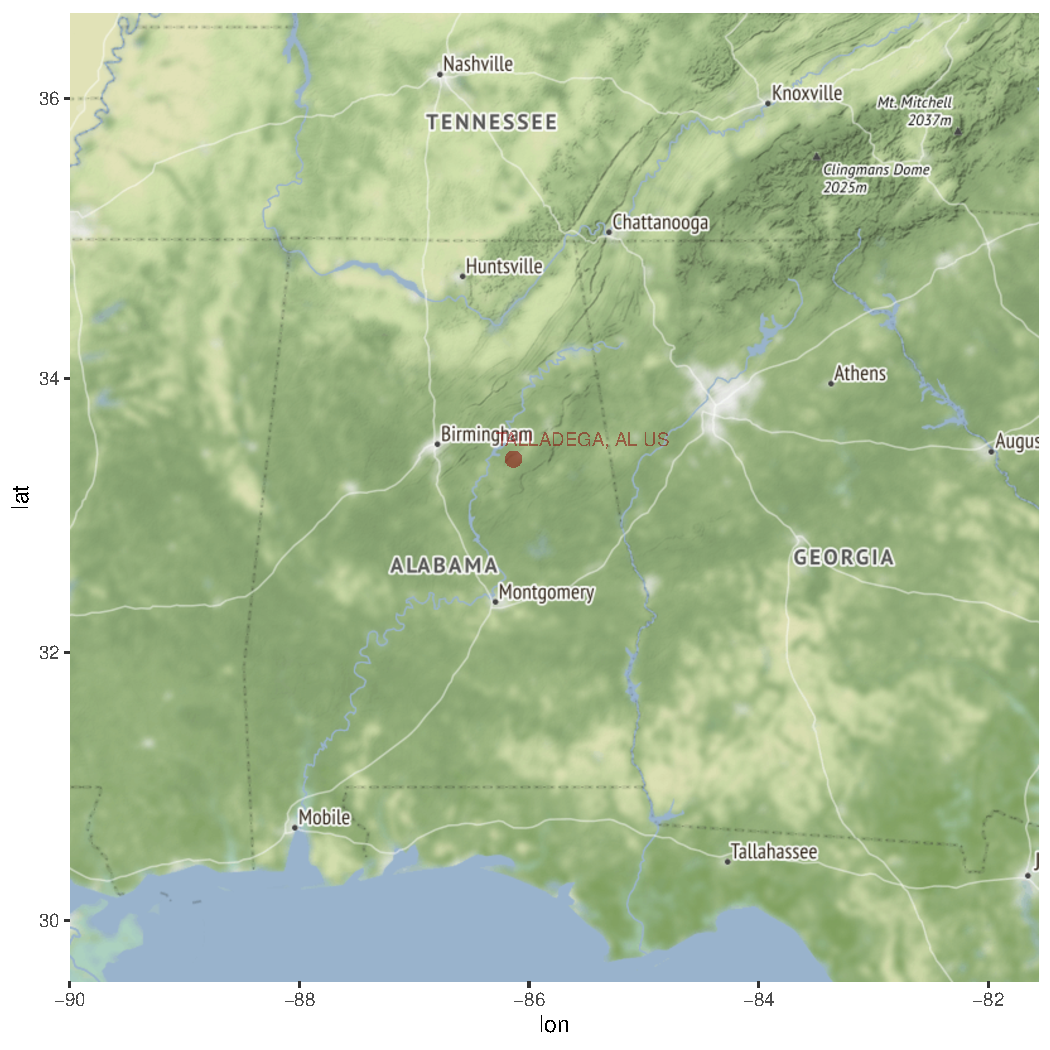
\includegraphics[width=\maxwidth]{figure/mapstation-1} 
\begin{kframe}\begin{alltt}
\hlcom{#zoom = 11, scale = 2, maptype ='watercolor',}

\hlkwd{png}\hlstd{(}\hlkwd{paste0}\hlstd{(}\hlstr{"png//"}\hlstd{, fips}\hlopt{$}\hlstd{State,} \hlstr{"-"}\hlstd{, stid,} \hlstr{"-MAP.png"}\hlstd{),}
    \hlkwc{width} \hlstd{=} \hlnum{480}\hlstd{,} \hlkwc{height} \hlstd{=} \hlnum{480}\hlstd{,} \hlkwc{units} \hlstd{=} \hlstr{"px"}\hlstd{,}
    \hlkwc{pointsize} \hlstd{=} \hlnum{12}\hlstd{,} \hlkwc{bg} \hlstd{=} \hlstr{"white"}\hlstd{)}

\hlcom{# For PNG?}
\hlkwd{ggmap}\hlstd{(myMap)}\hlopt{+}
\hlkwd{geom_point}\hlstd{(}\hlkwd{aes}\hlstd{(}\hlkwc{x} \hlstd{= lon,} \hlkwc{y} \hlstd{= lat),} \hlkwc{data} \hlstd{= station.df,}
   \hlkwc{alpha} \hlstd{=} \hlnum{.5}\hlstd{,} \hlkwc{color}\hlstd{=}\hlstr{"darkred"}\hlstd{,} \hlkwc{size} \hlstd{=} \hlnum{3}\hlstd{)} \hlopt{+}
   \hlkwd{geom_text}\hlstd{(}\hlkwd{aes}\hlstd{(}\hlkwc{x} \hlstd{= lon,} \hlkwc{y} \hlstd{= lat,} \hlkwc{label}\hlstd{=Station),}
      \hlkwc{data} \hlstd{= station.df,} \hlkwc{alpha} \hlstd{=} \hlnum{.5}\hlstd{,} \hlkwc{color}\hlstd{=}\hlstr{"darkred"}\hlstd{,}
      \hlkwc{size} \hlstd{=} \hlnum{3}\hlstd{,} \hlkwc{hjust}\hlstd{=}\hlnum{.1}\hlstd{,} \hlkwc{vjust}\hlstd{=}\hlopt{-}\hlnum{1}\hlstd{)}
\hlkwd{dev.off}\hlstd{()}
\end{alltt}
\begin{verbatim}
## pdf 
##   2
\end{verbatim}
\end{kframe}
\end{knitrout}

\subsection{Using a Linear Model Monthy Trends}

I used a linear model (\texttt{lm()}) to evaluate the long term trend for each each month to determine which, if any, have long-term trends. At somepoint, I'll have to the stats correcting for the autocorrelation using a autoregressive model.  



Evaluate both TMAX and TMIN in GSOM by Year using MonthEvalStats() function. 

\begin{knitrout}
\definecolor{shadecolor}{rgb}{0.969, 0.969, 0.969}\color{fgcolor}\begin{kframe}
\begin{alltt}
\hlstd{MonthEvalStatsOLD} \hlkwb{<-} \hlkwa{function}\hlstd{(}\hlkwc{GSOM}\hlstd{) \{}
\hlstd{sumstats} \hlkwb{=} \hlnum{NA}
\hlkwa{for} \hlstd{(m} \hlkwa{in} \hlnum{1}\hlopt{:}\hlnum{12}\hlstd{)\{}
  \hlstd{TMIN.lm} \hlkwb{=} \hlkwd{lm}\hlstd{(TMIN}\hlopt{~}\hlstd{Date, GSOM[GSOM}\hlopt{$}\hlstd{Month}\hlopt{==}\hlstd{m,])}
  \hlstd{TMAX.lm} \hlkwb{=} \hlkwd{lm}\hlstd{(TMAX}\hlopt{~}\hlstd{Date, GSOM[GSOM}\hlopt{$}\hlstd{Month}\hlopt{==}\hlstd{m,])}
   \hlstd{PPT.lm}  \hlkwb{=} \hlkwd{lm}\hlstd{(PPT}\hlopt{~}\hlstd{Date, GSOM[GSOM}\hlopt{$}\hlstd{Month}\hlopt{==}\hlstd{m,])}

 \hlstd{sumstats} \hlkwb{=} \hlkwd{rbind}\hlstd{(sumstats,}
   \hlkwd{data.frame}\hlstd{(}\hlkwc{Month} \hlstd{= m,} \hlkwc{Param}\hlstd{=}\hlstr{"TMIN"}\hlstd{,} \hlkwc{Slope} \hlstd{=} \hlkwd{coef}\hlstd{(TMIN.lm)[}\hlnum{2}\hlstd{],}
   \hlkwc{r2} \hlstd{=} \hlkwd{summary}\hlstd{(TMIN.lm)}\hlopt{$}\hlstd{r.squared,} \hlkwc{p_value}\hlstd{=} \hlkwd{anova}\hlstd{(TMIN.lm)}\hlopt{$}\hlstr{'Pr(>F)'}\hlstd{[}\hlnum{1}\hlstd{]),}
   \hlkwd{data.frame}\hlstd{(}\hlkwc{Month} \hlstd{= m,} \hlkwc{Param}\hlstd{=}\hlstr{"TMAX"}\hlstd{,} \hlkwc{Slope} \hlstd{=} \hlkwd{coef}\hlstd{(TMAX.lm)[}\hlnum{2}\hlstd{],}
   \hlkwc{r2} \hlstd{=} \hlkwd{summary}\hlstd{(TMAX.lm)}\hlopt{$}\hlstd{r.squared,} \hlkwc{p_value}\hlstd{=} \hlkwd{anova}\hlstd{(TMAX.lm)}\hlopt{$}\hlstr{'Pr(>F)'}\hlstd{[}\hlnum{1}\hlstd{]),}
   \hlkwd{data.frame}\hlstd{(}\hlkwc{Month}\hlstd{= m,} \hlkwc{Param}\hlstd{=}\hlstr{"PPT"}\hlstd{,} \hlkwc{Slope} \hlstd{=} \hlkwd{coef}\hlstd{(PPT.lm)[}\hlnum{2}\hlstd{],}
   \hlkwc{r2} \hlstd{=} \hlkwd{summary}\hlstd{(PPT.lm)}\hlopt{$}\hlstd{r.squared,} \hlkwc{p_value}\hlstd{=} \hlkwd{anova}\hlstd{(PPT.lm)}\hlopt{$}\hlstr{'Pr(>F)'}\hlstd{[}\hlnum{1}\hlstd{]))}

\hlstd{\}}

\hlstd{sumstats}\hlkwb{=}\hlkwd{data.frame}\hlstd{(sumstats)[}\hlopt{-}\hlnum{1}\hlstd{,]}
\hlkwd{rownames}\hlstd{(sumstats)}\hlkwb{<-}\hlkwa{NULL}

\hlstd{sumstats}\hlopt{$}\hlstd{Symbol} \hlkwb{=} \hlstr{""}
\hlstd{sumstats}\hlopt{$}\hlstd{Symbol[sumstats}\hlopt{$}\hlstd{p_value} \hlopt{<} \hlnum{0.05}\hlstd{]} \hlkwb{=} \hlstr{"*"}
\hlstd{sumstats}\hlopt{$}\hlstd{Symbol[sumstats}\hlopt{$}\hlstd{p_value} \hlopt{<} \hlnum{0.01}\hlstd{]} \hlkwb{=} \hlstr{"**"}
\hlstd{sumstats}\hlopt{$}\hlstd{Symbol[sumstats}\hlopt{$}\hlstd{p_value} \hlopt{<} \hlnum{0.001}\hlstd{]} \hlkwb{=} \hlstr{"***"}
\hlstd{sumstats[,}\hlkwd{c}\hlstd{(}\hlnum{7}\hlstd{,}\hlnum{9}\hlstd{)]}
\hlkwd{return}\hlstd{(sumstats)}
\hlstd{\}}

\hlstd{MonthEvalStats} \hlkwb{<-} \hlkwa{function}\hlstd{(}\hlkwc{GSOM}\hlstd{) \{}
\hlstd{sumstats} \hlkwb{=} \hlnum{NA}
\hlkwa{for} \hlstd{(m} \hlkwa{in} \hlnum{1}\hlopt{:}\hlnum{12}\hlstd{)\{}
  \hlstd{TMIN.lm} \hlkwb{=} \hlkwd{lm}\hlstd{(TMIN}\hlopt{~}\hlstd{Date, GSOM[GSOM}\hlopt{$}\hlstd{Month}\hlopt{==}\hlstd{m,])}
  \hlstd{TMAX.lm} \hlkwb{=} \hlkwd{lm}\hlstd{(TMAX}\hlopt{~}\hlstd{Date, GSOM[GSOM}\hlopt{$}\hlstd{Month}\hlopt{==}\hlstd{m,])}
   \hlstd{PPT.lm}  \hlkwb{=} \hlkwd{lm}\hlstd{(PPT}\hlopt{~}\hlstd{Date, GSOM[GSOM}\hlopt{$}\hlstd{Month}\hlopt{==}\hlstd{m,])}

 \hlstd{sumstats} \hlkwb{=} \hlkwd{rbind}\hlstd{(sumstats,}
   \hlkwd{data.frame}\hlstd{(}\hlkwc{Month} \hlstd{= m,} \hlkwc{Param}\hlstd{=}\hlstr{"TMIN"}\hlstd{,} \hlkwc{Slope} \hlstd{=} \hlkwd{coef}\hlstd{(TMIN.lm)[}\hlnum{2}\hlstd{],}
   \hlkwc{r2} \hlstd{=} \hlkwd{summary}\hlstd{(TMIN.lm)}\hlopt{$}\hlstd{r.squared,} \hlkwc{p_value}\hlstd{=} \hlkwd{anova}\hlstd{(TMIN.lm)}\hlopt{$}\hlstr{'Pr(>F)'}\hlstd{[}\hlnum{1}\hlstd{]),}
   \hlkwd{data.frame}\hlstd{(}\hlkwc{Month} \hlstd{= m,} \hlkwc{Param}\hlstd{=}\hlstr{"TMAX"}\hlstd{,} \hlkwc{Slope} \hlstd{=} \hlkwd{coef}\hlstd{(TMAX.lm)[}\hlnum{2}\hlstd{],}
   \hlkwc{r2} \hlstd{=} \hlkwd{summary}\hlstd{(TMAX.lm)}\hlopt{$}\hlstd{r.squared,} \hlkwc{p_value}\hlstd{=} \hlkwd{anova}\hlstd{(TMAX.lm)}\hlopt{$}\hlstr{'Pr(>F)'}\hlstd{[}\hlnum{1}\hlstd{]),}
   \hlkwd{data.frame}\hlstd{(}\hlkwc{Month}\hlstd{= m,} \hlkwc{Param}\hlstd{=}\hlstr{"PPT"}\hlstd{,} \hlkwc{Slope} \hlstd{=} \hlkwd{coef}\hlstd{(PPT.lm)[}\hlnum{2}\hlstd{],}
   \hlkwc{r2} \hlstd{=} \hlkwd{summary}\hlstd{(PPT.lm)}\hlopt{$}\hlstd{r.squared,} \hlkwc{p_value}\hlstd{=} \hlkwd{anova}\hlstd{(PPT.lm)}\hlopt{$}\hlstr{'Pr(>F)'}\hlstd{[}\hlnum{1}\hlstd{]))}

\hlstd{\}} \hlcom{#end loop}

\hlstd{sumstats}\hlkwb{=}\hlkwd{data.frame}\hlstd{(sumstats)[}\hlopt{-}\hlnum{1}\hlstd{,]}
\hlkwd{rownames}\hlstd{(sumstats)}\hlkwb{<-}\hlkwa{NULL}
\hlkwd{head}\hlstd{(sumstats)}

\hlstd{sumstats}\hlopt{$}\hlstd{Symbol} \hlkwb{=} \hlstr{""}
\hlstd{sumstats}\hlopt{$}\hlstd{Symbol[sumstats}\hlopt{$}\hlstd{p_value} \hlopt{<} \hlnum{0.05}\hlstd{]} \hlkwb{=} \hlstr{"*"}
\hlstd{sumstats}\hlopt{$}\hlstd{Symbol[sumstats}\hlopt{$}\hlstd{p_value} \hlopt{<} \hlnum{0.01}\hlstd{]} \hlkwb{=} \hlstr{"**"}
\hlstd{sumstats}\hlopt{$}\hlstd{Symbol[sumstats}\hlopt{$}\hlstd{p_value} \hlopt{<} \hlnum{0.001}\hlstd{]} \hlkwb{=} \hlstr{"***"}
\hlkwd{return}\hlstd{(sumstats)}
\hlstd{\}}

\hlcom{# test function}
\hlstd{sumstats} \hlkwb{=} \hlkwd{MonthEvalStats}\hlstd{(GSOM[}\hlnum{500}\hlopt{:}\hlnum{4000}\hlstd{,])}
\end{alltt}
\end{kframe}
\end{knitrout}


\subsubsection{Trends in Tabular Formats}

Admittedly, determining the months with the biggest changes isn't a very good approach for hypothesize testing -- it's more like a fishing expedition, but as long as we understand the difference between an a priori hypothesis and an exploratory analysis, we should be okay if we make appropriate conclusions. 

\begin{knitrout}
\definecolor{shadecolor}{rgb}{0.969, 0.969, 0.969}\color{fgcolor}\begin{kframe}
\begin{alltt}
\hlcom{# Selecting Most Important Monthly Changes (TMAX overwrites)}
\hlcom{#sumstats = MonthEvalStats(GSOM)}

\hlstd{TMIN_Increase_month} \hlkwb{=} \hlkwd{with}\hlstd{(sumstats[sumstats}\hlopt{$}\hlstd{Param}\hlopt{==}\hlstr{"TMIN"}\hlstd{,],}
     \hlstd{Month[Slope}\hlopt{==}\hlkwd{max}\hlstd{(Slope,} \hlkwc{na.rm}\hlstd{=T)])}
\hlstd{TMIN_Decrease_month} \hlkwb{=} \hlkwd{with}\hlstd{(sumstats[sumstats}\hlopt{$}\hlstd{Param}\hlopt{==}\hlstr{"TMIN"}\hlstd{,],}
     \hlstd{Month[Slope}\hlopt{==}\hlkwd{min}\hlstd{(Slope,} \hlkwc{na.rm}\hlstd{=T)])}
\hlstd{TMAX_Increase_month} \hlkwb{=} \hlkwd{with}\hlstd{(sumstats[sumstats}\hlopt{$}\hlstd{Param}\hlopt{==}\hlstr{"TMAX"}\hlstd{,],}
     \hlstd{Month[Slope}\hlopt{==}\hlkwd{max}\hlstd{(Slope,} \hlkwc{na.rm}\hlstd{=T)])}
\hlstd{TMAX_Decrease_month} \hlkwb{=} \hlkwd{with}\hlstd{(sumstats[sumstats}\hlopt{$}\hlstd{Param}\hlopt{==}\hlstr{"TMAX"}\hlstd{,],}
     \hlstd{Month[Slope}\hlopt{==}\hlkwd{min}\hlstd{(Slope,} \hlkwc{na.rm}\hlstd{=T)])}
\hlstd{PPT_Increase_month} \hlkwb{=} \hlkwd{with}\hlstd{(sumstats[sumstats}\hlopt{$}\hlstd{Param}\hlopt{==}\hlstr{"PPT"}\hlstd{,],}
     \hlstd{Month[Slope}\hlopt{==}\hlkwd{max}\hlstd{(Slope,} \hlkwc{na.rm}\hlstd{=T)])}
\hlstd{PPT_Decrease_month} \hlkwb{=} \hlkwd{with}\hlstd{(sumstats[sumstats}\hlopt{$}\hlstd{Param}\hlopt{==}\hlstr{"PPT"}\hlstd{,],}
     \hlstd{Month[Slope}\hlopt{==}\hlkwd{min}\hlstd{(Slope,} \hlkwc{na.rm}\hlstd{=T)])}
\end{alltt}
\end{kframe}
\end{knitrout}

For this section, we'll look to see what months had the greatest changes for both TMIN and TMAX. By looking at significant slopes in whatever direction, we might learn if warming is really the dominiant pattern. 

Table~\ref{tab:TMINtrends} summarizes the monthly trends for TMAX.

\begin{kframe}


{\ttfamily\noindent\bfseries\color{errorcolor}{\#\# Error in print.xtable(TMIN.xtbl, type = "{}latex"{}, comment = FALSE, caption = "{}Montly TMIN Trends"{}, : argument 4 matches multiple formal arguments}}\end{kframe}

Table~\ref{tab:TMAXtrends} summarizes the monthly trends for TMAX.

\begin{kframe}


{\ttfamily\noindent\bfseries\color{errorcolor}{\#\# Error in print.xtable(TMAX.xtbl, type = "{}latex"{}, comment = FALSE, caption = "{}TMAX Trends by Month"{}, : argument 4 matches multiple formal arguments}}\end{kframe}

PPT changes are tricky to capture and I'll have to keep working on this (Table~\ref{tab:PPTtrends}).

\begin{kframe}


{\ttfamily\noindent\bfseries\color{errorcolor}{\#\# Error in print.xtable(PPT.xtbl, type = "{}latex"{}, caption = "{}Precipitation Trends by Month"{}, : argument 3 matches multiple formal arguments}}\end{kframe}

\subsubsection{Defining TMAXmonth and TMINmonth}

\begin{knitrout}
\definecolor{shadecolor}{rgb}{0.969, 0.969, 0.969}\color{fgcolor}\begin{kframe}
\begin{alltt}
\hlstd{TMINSlopeMax} \hlkwb{=} \hlkwd{max}\hlstd{(}\hlkwd{abs}\hlstd{(sumstats}\hlopt{$}\hlstd{Slope)[sumstats}\hlopt{$}\hlstd{Param}\hlopt{==}\hlstr{"TMIN"}\hlstd{])}
\hlstd{TMAXSlopeMax} \hlkwb{=} \hlkwd{max}\hlstd{(}\hlkwd{abs}\hlstd{(sumstats}\hlopt{$}\hlstd{Slope)[sumstats}\hlopt{$}\hlstd{Param}\hlopt{==}\hlstr{"TMAX"}\hlstd{])}

\hlstd{TMINmonthMax} \hlkwb{=} \hlkwd{as.numeric}\hlstd{(}\hlkwd{subset}\hlstd{(sumstats,} \hlkwc{select}\hlstd{=Month,} \hlkwc{subset}\hlstd{=}\hlkwd{abs}\hlstd{(Slope)}\hlopt{==}\hlstd{TMINSlopeMax))}

\hlstd{TMAXmonthMax} \hlkwb{=} \hlkwd{as.numeric}\hlstd{(}\hlkwd{subset}\hlstd{(sumstats,} \hlkwc{select}\hlstd{=Month,} \hlkwc{subset}\hlstd{=}\hlkwd{abs}\hlstd{(Slope)}\hlopt{==}\hlstd{TMAXSlopeMax))}
\end{alltt}
\end{kframe}
\end{knitrout}
The greatest changes for Station GHCND:USC00018024

\section{Communicating Long-term Weather Records}

\subsection{Complete Records vs. Post 1975 Trends}

Communicating climate change based on station records is tricky. The long-term record would on the surface to be the most robust, but several issues arise with a naive analytical approach -- my favorite!

\begin{knitrout}
\definecolor{shadecolor}{rgb}{0.969, 0.969, 0.969}\color{fgcolor}\begin{kframe}
\begin{alltt}
\hlkwd{setwd}\hlstd{(}\hlstr{"/home/CAMPUS/mwl04747/github/Climate_Change_Narratives/"}\hlstd{)}

\hlstd{GSOM_1975.png} \hlkwb{=} \hlkwd{paste0}\hlstd{(fips}\hlopt{$}\hlstd{State,} \hlstr{"-"}\hlstd{, stid,} \hlstr{"-GSOM_1975.png"}\hlstd{)}

\hlkwd{png}\hlstd{(}\hlkwd{paste0}\hlstd{(png_public, GSOM_1975.png),} \hlkwc{width} \hlstd{=} \hlnum{480}\hlstd{,} \hlkwc{height} \hlstd{=} \hlnum{320}\hlstd{,} \hlkwc{units} \hlstd{=} \hlstr{"px"}\hlstd{,} \hlkwc{pointsize} \hlstd{=} \hlnum{12}\hlstd{,} \hlkwc{bg} \hlstd{=} \hlstr{"white"}\hlstd{)}
\end{alltt}


{\ttfamily\noindent\bfseries\color{errorcolor}{\#\# Error in paste0(png\_public, GSOM\_1975.png): object 'png\_public' not found}}\begin{alltt}
\hlkwd{par}\hlstd{(}\hlkwc{las}\hlstd{=}\hlnum{1}\hlstd{,} \hlkwc{mfrow}\hlstd{=}\hlkwd{c}\hlstd{(}\hlnum{1}\hlstd{,}\hlnum{1}\hlstd{))}
\hlkwd{plot}\hlstd{(TMAX}\hlopt{~}\hlstd{Date, GSOM,} \hlkwc{pch}\hlstd{=}\hlnum{20}\hlstd{,} \hlkwc{cex}\hlstd{=}\hlnum{.5}\hlstd{,} \hlkwc{col}\hlstd{=}\hlstr{"grey"}\hlstd{,} \hlkwc{ylab}\hlstd{=}\hlstr{"°F"}\hlstd{,} \hlkwc{main}\hlstd{=}\hlkwd{paste0}\hlstd{(fips}\hlopt{$}\hlstd{State,} \hlstr{"-"}\hlstd{, stid))}
\hlstd{GSOM.lm} \hlkwb{=} \hlkwd{lm}\hlstd{(TMAX}\hlopt{~}\hlstd{Date, GSOM)}
\hlstd{pred_dates} \hlkwb{<-}\hlkwd{data.frame}\hlstd{(}\hlkwc{Date} \hlstd{= GSOM}\hlopt{$}\hlstd{Date);}
\hlkwd{nrow}\hlstd{(pred_dates);}\hlcom{# pred_dates}
\end{alltt}
\begin{verbatim}
## [1] 1369
\end{verbatim}
\begin{alltt}
\hlcom{#Predits the values with confidence interval }
\hlstd{ci} \hlkwb{<-} \hlkwd{predict}\hlstd{(GSOM.lm,} \hlkwc{newdata} \hlstd{= pred_dates,}
              \hlkwc{interval} \hlstd{=} \hlstr{'confidence'}\hlstd{)}
\hlkwd{lines}\hlstd{(pred_dates}\hlopt{$}\hlstd{Date,} \hlkwd{as.numeric}\hlstd{(ci[,}\hlnum{1}\hlstd{]),} \hlkwc{col}\hlstd{=}\hlstr{"gray50"}\hlstd{)}

\hlcom{# Post 1975}
\hlstd{GSOM.lm} \hlkwb{=} \hlkwd{lm}\hlstd{(TMAX}\hlopt{~}\hlstd{Date, GSOM[GSOM}\hlopt{$}\hlstd{Year}\hlopt{>}\hlnum{1975}\hlstd{,])}
\hlstd{pred_dates} \hlkwb{<-}\hlkwd{data.frame}\hlstd{(}\hlkwc{Date} \hlstd{= GSOM}\hlopt{$}\hlstd{Date[GSOM}\hlopt{$}\hlstd{Year}\hlopt{>}\hlnum{1975}\hlstd{]);}
\hlkwd{nrow}\hlstd{(pred_dates);} \hlcom{#pred_dates}
\end{alltt}
\begin{verbatim}
## [1] 510
\end{verbatim}
\begin{alltt}
\hlcom{#Predits the values with confidence interval }
\hlstd{ci} \hlkwb{<-} \hlkwd{predict}\hlstd{(GSOM.lm,} \hlkwc{newdata} \hlstd{= pred_dates,}
              \hlkwc{interval} \hlstd{=} \hlstr{'confidence'}\hlstd{)}
\hlkwd{lines}\hlstd{(pred_dates}\hlopt{$}\hlstd{Date,} \hlkwd{as.numeric}\hlstd{(ci[,}\hlnum{1}\hlstd{]),} \hlkwc{col}\hlstd{=}\hlstr{"red"}\hlstd{)}
\hlkwd{lines}\hlstd{(pred_dates}\hlopt{$}\hlstd{Date,} \hlkwd{as.numeric}\hlstd{(ci[,}\hlnum{2}\hlstd{]),} \hlkwc{col}\hlstd{=}\hlstr{"darkorange"}\hlstd{)}
\hlkwd{lines}\hlstd{(pred_dates}\hlopt{$}\hlstd{Date, ci[,}\hlnum{3}\hlstd{],} \hlkwc{col}\hlstd{=}\hlstr{"darkorange"}\hlstd{)}
\hlstd{location_index} \hlkwb{=} \hlkwd{round}\hlstd{(}\hlkwd{length}\hlstd{(GSOM[GSOM}\hlopt{$}\hlstd{Year}\hlopt{>}\hlnum{1975}\hlstd{,]}\hlopt{$}\hlstd{Date)} \hlopt{*} \hlnum{0.99}\hlstd{,}\hlnum{0}\hlstd{)}
\hlkwd{text}\hlstd{(pred_dates}\hlopt{$}\hlstd{Date[location_index], ci[location_index,}\hlnum{3}\hlstd{],}
     \hlkwd{paste}\hlstd{(}\hlkwd{report_prob3}\hlstd{(GSOM.lm))[}\hlnum{2}\hlstd{],} \hlkwc{pos}\hlstd{=}\hlnum{2}\hlstd{,} \hlkwc{cex}\hlstd{=}\hlnum{1.0}\hlstd{,} \hlkwc{col}\hlstd{=}\hlstr{"red"}\hlstd{)}
\end{alltt}
\end{kframe}
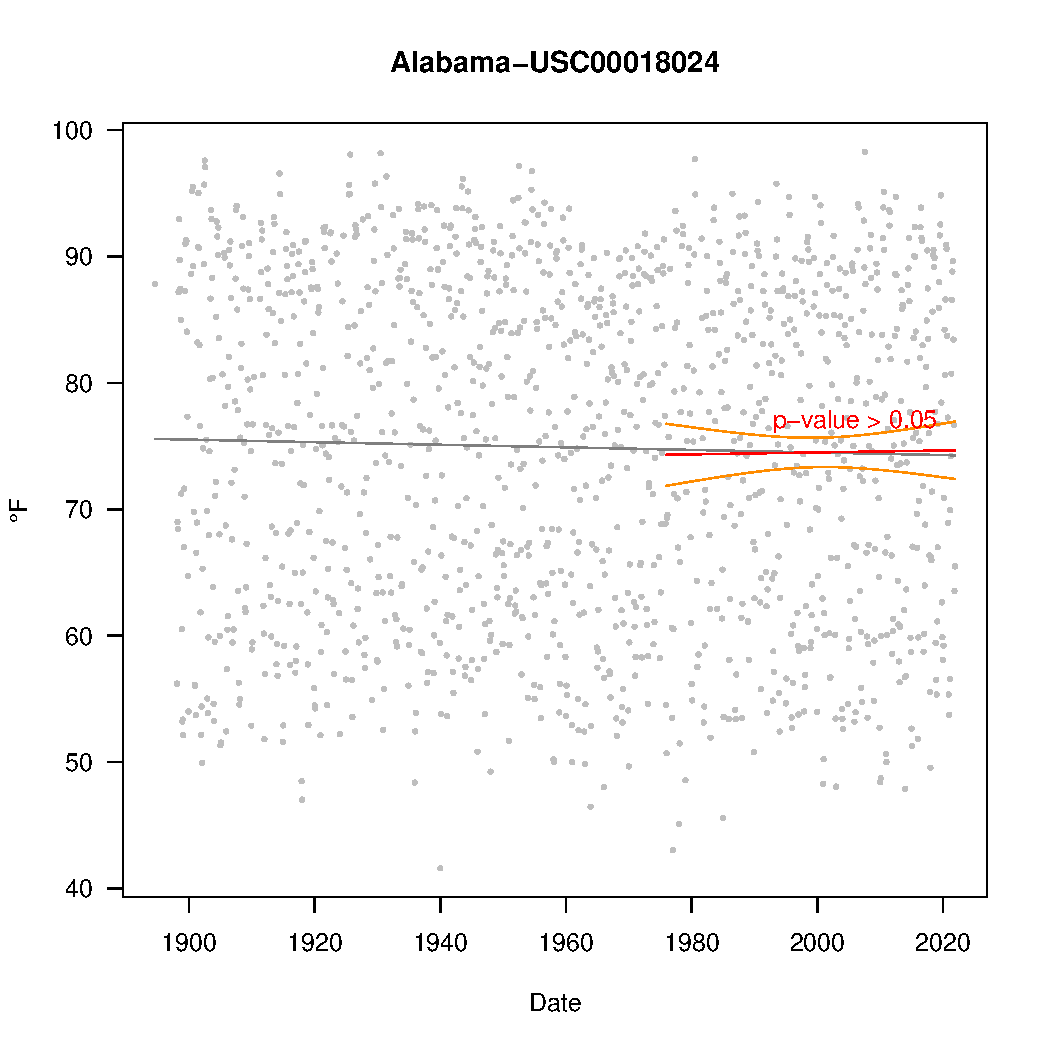
\includegraphics[width=\maxwidth]{figure/trend1975-1} 
\begin{kframe}\begin{alltt}
\hlcom{#abline(coef(lm(TMAX~Date, GSOM)), col="black")}
\hlcom{#abline(coef(lm(TMAX~Date, GSOM[GSOM$Year>1975,])), col="red")}
\hlkwd{dev.off}\hlstd{()}
\end{alltt}
\begin{verbatim}
## null device 
##           1
\end{verbatim}
\end{kframe}
\end{knitrout}

The noise in the data may suggests that no trend is present (Figure~\ref{fig:GSOM-1975trend}). It's tricky because the seasonal variation dominates the source of varition. In other words the intra-annual variation exceeds the inter-annual variation, making signal detection very difficult. Is there a way to "filter" out the seasonal effect? Yes, let's see how that works next. 

\begin{figure}
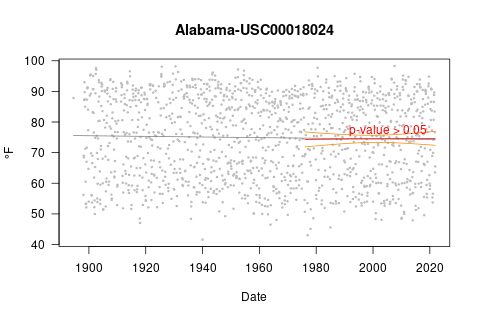
\includegraphics[width=1.00\textwidth]{/home/CAMPUS/mwl04747/github/Climate_Change_Narratives/Social_Media/png/Alabama-USC00018024-GSOMmonthly1975.png}
\caption{The climate trends from full record and post 1975 data. These data have a high level of variability due to seasonality effects that have not been filtered out.}
\label{fig:GSOM-1975trend}
\end{figure}


\subsection{Filtering Seasonal Effect}

There are several ways to filter out seasonal effects. The easiest way is subtract the mean value for each date, but that's tricky because every four years there is an extra day in Februrary -- although there are ways to deal with this, a more straight forward way is to use mean monthly values to capture the seasonality for each month. With 12 months, this is a pretty good approach because there is pretty good resolution. 

\subsubsection{Method 1 Filtering by Monthly Mean} 

\begin{knitrout}
\definecolor{shadecolor}{rgb}{0.969, 0.969, 0.969}\color{fgcolor}\begin{kframe}
\begin{alltt}
\hlstd{TMAX.Monthly.means} \hlkwb{=} \hlkwd{aggregate}\hlstd{(TMAX}\hlopt{~}\hlstd{Month,} \hlkwc{data}\hlstd{=GSOM, mean)}
\hlkwd{names}\hlstd{(TMAX.Monthly.means)}\hlkwb{=}\hlkwd{c}\hlstd{(}\hlstr{"Month"}\hlstd{,} \hlstr{"TMAXmean"}\hlstd{)}
\hlstd{GSOM2} \hlkwb{=} \hlkwd{merge}\hlstd{(GSOM, TMAX.Monthly.means,} \hlkwc{by}\hlstd{=}\hlstr{"Month"}\hlstd{)}
\hlstd{GSOM2}\hlopt{$}\hlstd{TMAX.anom} \hlkwb{=} \hlstd{GSOM2}\hlopt{$}\hlstd{TMAX} \hlopt{-} \hlstd{GSOM2}\hlopt{$}\hlstd{TMAXmean}

\hlstd{TMIN.Monthly.means} \hlkwb{=} \hlkwd{aggregate}\hlstd{(TMIN}\hlopt{~}\hlstd{Month, GSOM, mean)}
\hlkwd{names}\hlstd{(TMIN.Monthly.means)}\hlkwb{=}\hlkwd{c}\hlstd{(}\hlstr{"Month"}\hlstd{,} \hlstr{"TMINmean"}\hlstd{)}
\hlstd{GSOM2} \hlkwb{=} \hlkwd{merge}\hlstd{(GSOM2, TMIN.Monthly.means,} \hlkwc{by}\hlstd{=}\hlstr{"Month"}\hlstd{)}
\hlstd{GSOM2}\hlopt{$}\hlstd{TMIN.anom} \hlkwb{=} \hlstd{GSOM2}\hlopt{$}\hlstd{TMIN} \hlopt{-} \hlstd{GSOM2}\hlopt{$}\hlstd{TMINmean}

\hlstd{PPT.Monthly.means} \hlkwb{=} \hlkwd{aggregate}\hlstd{(PPT}\hlopt{~}\hlstd{Month, GSOM, mean)}
\hlkwd{names}\hlstd{(PPT.Monthly.means)}\hlkwb{=}\hlkwd{c}\hlstd{(}\hlstr{"Month"}\hlstd{,} \hlstr{"PPTmean"}\hlstd{)}
\hlstd{GSOM2} \hlkwb{=} \hlkwd{merge}\hlstd{(GSOM2, PPT.Monthly.means,} \hlkwc{by}\hlstd{=}\hlstr{"Month"}\hlstd{)}
\hlstd{GSOM2}\hlopt{$}\hlstd{PPT.anom} \hlkwb{=} \hlstd{GSOM2}\hlopt{$}\hlstd{PPT} \hlopt{-} \hlstd{GSOM2}\hlopt{$}\hlstd{PPTmean}

\hlcom{# Sort by date}
\hlstd{GSOM2} \hlkwb{<-} \hlstd{GSOM2[}\hlkwd{order}\hlstd{(GSOM2}\hlopt{$}\hlstd{Date),]}
\end{alltt}
\end{kframe}
\end{knitrout}

\begin{knitrout}
\definecolor{shadecolor}{rgb}{0.969, 0.969, 0.969}\color{fgcolor}\begin{kframe}
\begin{alltt}
\hlstd{GSOM_anomaly.png} \hlkwb{=} \hlkwd{paste0}\hlstd{(fips}\hlopt{$}\hlstd{State,} \hlstr{"-"}\hlstd{, stid,} \hlstr{"-GSOM_anomaly1975.png"}\hlstd{)}

\hlkwd{png}\hlstd{(}\hlkwd{paste0}\hlstd{(png_public, GSOM_anomaly.png),}
    \hlkwc{width} \hlstd{=} \hlnum{480}\hlstd{,} \hlkwc{height} \hlstd{=} \hlnum{320}\hlstd{,} \hlkwc{units} \hlstd{=} \hlstr{"px"}\hlstd{,}
    \hlkwc{pointsize} \hlstd{=} \hlnum{12}\hlstd{,} \hlkwc{bg} \hlstd{=} \hlstr{"white"}\hlstd{)}
\end{alltt}


{\ttfamily\noindent\bfseries\color{errorcolor}{\#\# Error in paste0(png\_public, GSOM\_anomaly.png): object 'png\_public' not found}}\begin{alltt}
\hlkwd{par}\hlstd{(}\hlkwc{las}\hlstd{=}\hlnum{1}\hlstd{,} \hlkwc{mfrow}\hlstd{=}\hlkwd{c}\hlstd{(}\hlnum{1}\hlstd{,}\hlnum{1}\hlstd{))}
\hlkwd{par}\hlstd{(}\hlkwc{las}\hlstd{=}\hlnum{1}\hlstd{)}
\hlkwd{plot}\hlstd{(TMAX.anom}\hlopt{~}\hlstd{Date, GSOM2,} \hlkwc{pch}\hlstd{=}\hlnum{20}\hlstd{,} \hlkwc{cex}\hlstd{=}\hlnum{.5}\hlstd{,}
     \hlkwc{col}\hlstd{=}\hlstr{"grey"}\hlstd{,} \hlkwc{ylab}\hlstd{=}\hlstr{"Max. Temp (anomaly) °F"}\hlstd{,}
     \hlkwc{main}\hlstd{=}\hlkwd{paste0}\hlstd{(}\hlstr{"Seasonally Filtered"}\hlstd{, fips}\hlopt{$}\hlstd{State,} \hlstr{" ("}\hlstd{, stid,} \hlstr{")"}\hlstd{,}
         \hlkwd{report_prob3}\hlstd{(GSOM.lm)[}\hlnum{3}\hlstd{]))}
\hlstd{GSOM.lm} \hlkwb{=} \hlkwd{lm}\hlstd{(TMAX.anom}\hlopt{~}\hlstd{Date, GSOM2)}
\hlstd{pred_dates} \hlkwb{<-}\hlkwd{data.frame}\hlstd{(}\hlkwc{Date} \hlstd{= GSOM2}\hlopt{$}\hlstd{Date);}
\hlkwd{nrow}\hlstd{(pred_dates);} \hlcom{#pred_dates}
\end{alltt}
\begin{verbatim}
## [1] 1369
\end{verbatim}
\begin{alltt}
\hlcom{#Predits the values with confidence interval }
\hlstd{ci} \hlkwb{<-} \hlkwd{predict}\hlstd{(GSOM.lm,} \hlkwc{newdata} \hlstd{= pred_dates,}
              \hlkwc{interval} \hlstd{=} \hlstr{'confidence'}\hlstd{)}
\hlkwd{lines}\hlstd{(pred_dates}\hlopt{$}\hlstd{Date,} \hlkwd{as.numeric}\hlstd{(ci[,}\hlnum{1}\hlstd{]),} \hlkwc{col}\hlstd{=}\hlstr{"gray50"}\hlstd{)}

\hlstd{ymax}\hlkwb{=}\hlkwd{max}\hlstd{(GSOM2}\hlopt{$}\hlstd{TMAX.anom)} \hlopt{-} \hlstd{(}\hlkwd{max}\hlstd{(GSOM2}\hlopt{$}\hlstd{TMAX.anom)}\hlopt{-}\hlkwd{min}\hlstd{(GSOM2}\hlopt{$}\hlstd{TMAX.anom))}\hlopt{*}\hlnum{.3}
\hlstd{ymax2} \hlkwb{<-} \hlstd{ymax} \hlopt{-} \hlstd{(}\hlkwd{max}\hlstd{(GSOM2}\hlopt{$}\hlstd{TMAX.anom)}\hlopt{-}\hlkwd{min}\hlstd{(GSOM2}\hlopt{$}\hlstd{TMAX.anom))}\hlopt{*}\hlnum{.1}

\hlstd{location_index} \hlkwb{=} \hlkwd{round}\hlstd{(}\hlkwd{length}\hlstd{(GSOM2[GSOM2}\hlopt{$}\hlstd{Year}\hlopt{>}\hlnum{1975}\hlstd{,]}\hlopt{$}\hlstd{Date)} \hlopt{*} \hlnum{0.99}\hlstd{,}\hlnum{3}\hlstd{)}
\hlkwd{text}\hlstd{(pred_dates}\hlopt{$}\hlstd{Date[location_index], ymax,}
     \hlkwd{paste}\hlstd{(}\hlkwd{report_prob3}\hlstd{(GSOM.lm))[}\hlnum{1}\hlstd{],} \hlkwc{pos}\hlstd{=}\hlnum{2}\hlstd{,} \hlkwc{cex}\hlstd{=}\hlnum{.9}\hlstd{)}
\hlkwd{text}\hlstd{(pred_dates}\hlopt{$}\hlstd{Date[location_index], ymax2,}
     \hlkwd{paste}\hlstd{(}\hlkwd{report_prob3}\hlstd{(GSOM.lm))[}\hlnum{2}\hlstd{],} \hlkwc{pos}\hlstd{=}\hlnum{2}\hlstd{,} \hlkwc{cex}\hlstd{=}\hlnum{.9}\hlstd{)}

\hlcom{# Post 1975}
\hlstd{GSOM.lm} \hlkwb{=} \hlkwd{lm}\hlstd{(TMAX.anom}\hlopt{~}\hlstd{Date, GSOM2[GSOM2}\hlopt{$}\hlstd{Year}\hlopt{>}\hlnum{1975}\hlstd{,])}
\hlstd{pred_dates} \hlkwb{<-}\hlkwd{data.frame}\hlstd{(}\hlkwc{Date} \hlstd{= GSOM2}\hlopt{$}\hlstd{Date[GSOM2}\hlopt{$}\hlstd{Year}\hlopt{>}\hlnum{1975}\hlstd{]);}
\hlkwd{nrow}\hlstd{(pred_dates);} \hlcom{#pred_dates}
\end{alltt}
\begin{verbatim}
## [1] 510
\end{verbatim}
\begin{alltt}
\hlcom{#Predits the values with confidence interval }
\hlstd{ci} \hlkwb{<-} \hlkwd{predict}\hlstd{(GSOM.lm,} \hlkwc{newdata} \hlstd{= pred_dates,}
              \hlkwc{interval} \hlstd{=} \hlstr{'confidence'}\hlstd{)}
\hlkwd{lines}\hlstd{(pred_dates}\hlopt{$}\hlstd{Date,} \hlkwd{as.numeric}\hlstd{(ci[,}\hlnum{1}\hlstd{]),} \hlkwc{col}\hlstd{=}\hlstr{"red"}\hlstd{)}
\hlkwd{lines}\hlstd{(pred_dates}\hlopt{$}\hlstd{Date,} \hlkwd{as.numeric}\hlstd{(ci[,}\hlnum{2}\hlstd{]),} \hlkwc{col}\hlstd{=}\hlstr{"darkorange"}\hlstd{)}
\hlkwd{lines}\hlstd{(pred_dates}\hlopt{$}\hlstd{Date, ci[,}\hlnum{3}\hlstd{],} \hlkwc{col}\hlstd{=}\hlstr{"darkorange"}\hlstd{)}

\hlstd{ymax}\hlkwb{=}\hlkwd{max}\hlstd{(GSOM2}\hlopt{$}\hlstd{TMAX.anom)} \hlopt{-} \hlstd{(}\hlkwd{max}\hlstd{(GSOM2}\hlopt{$}\hlstd{TMAX.anom)}\hlopt{-}\hlkwd{min}\hlstd{(GSOM2}\hlopt{$}\hlstd{TMAX.anom))}\hlopt{*}\hlnum{.7}
\hlstd{ymax2} \hlkwb{<-} \hlstd{ymax} \hlopt{-} \hlstd{(}\hlkwd{max}\hlstd{(GSOM2}\hlopt{$}\hlstd{TMAX.anom)}\hlopt{-}\hlkwd{min}\hlstd{(GSOM2}\hlopt{$}\hlstd{TMAX.anom))}\hlopt{*}\hlnum{.1}

\hlstd{location_index} \hlkwb{=} \hlkwd{round}\hlstd{(}\hlkwd{length}\hlstd{(GSOM2[GSOM2}\hlopt{$}\hlstd{Year}\hlopt{>}\hlnum{1975}\hlstd{,]}\hlopt{$}\hlstd{Date)} \hlopt{*} \hlnum{0.99}\hlstd{,}\hlnum{0}\hlstd{)}
\hlkwd{text}\hlstd{(pred_dates}\hlopt{$}\hlstd{Date[location_index], ymax,}
     \hlkwd{paste}\hlstd{(}\hlkwd{report_prob3}\hlstd{(GSOM.lm))[}\hlnum{1}\hlstd{],} \hlkwc{pos}\hlstd{=}\hlnum{2}\hlstd{,} \hlkwc{cex}\hlstd{=}\hlnum{.9}\hlstd{,} \hlkwc{col}\hlstd{=}\hlstr{"red"}\hlstd{)}
\hlkwd{text}\hlstd{(pred_dates}\hlopt{$}\hlstd{Date[location_index], ymax2,}
     \hlkwd{paste}\hlstd{(}\hlkwd{report_prob3}\hlstd{(GSOM.lm))[}\hlnum{2}\hlstd{],} \hlkwc{pos}\hlstd{=}\hlnum{2}\hlstd{,} \hlkwc{cex}\hlstd{=}\hlnum{.9}\hlstd{,} \hlkwc{col}\hlstd{=}\hlstr{"red"}\hlstd{)}
\end{alltt}
\end{kframe}
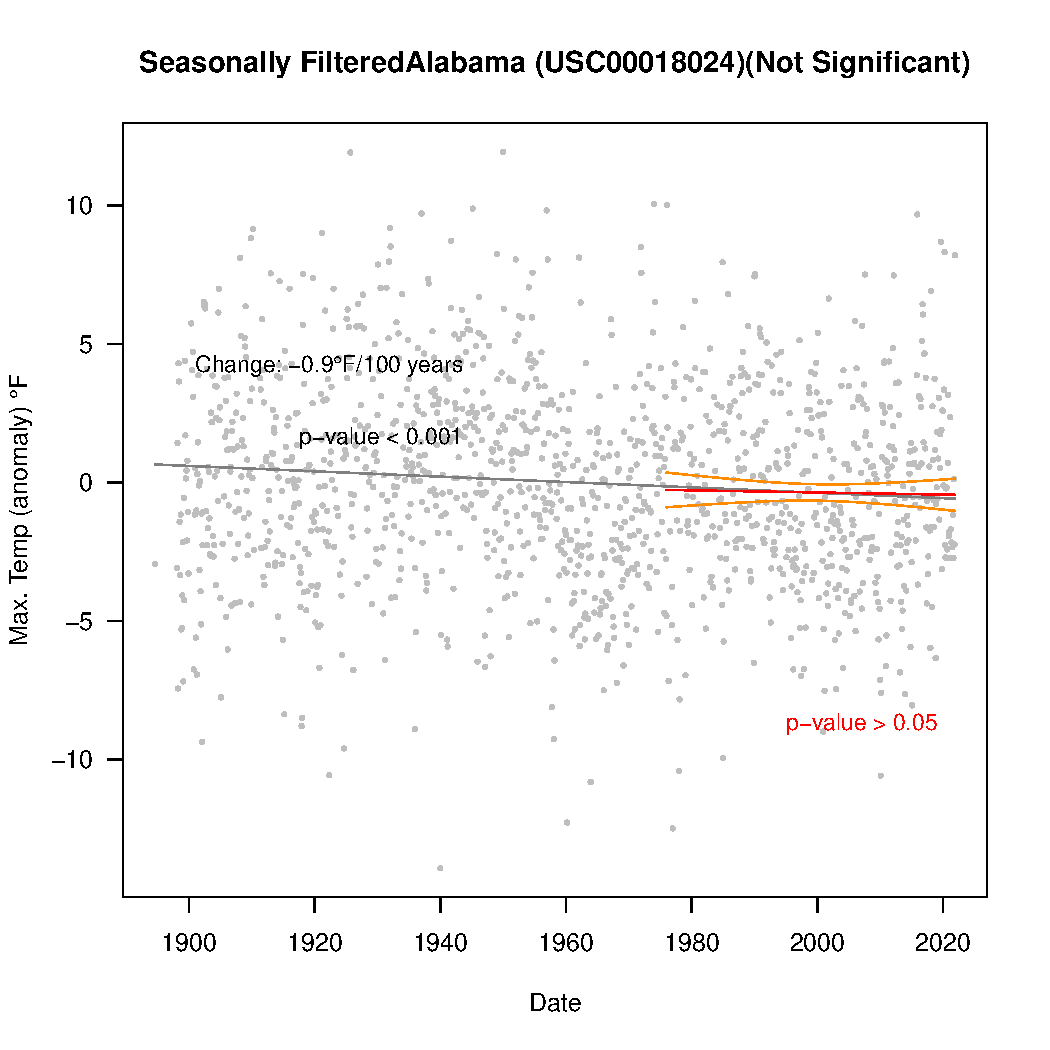
\includegraphics[width=\maxwidth]{figure/unnamed-chunk-8-1} 
\begin{kframe}\begin{alltt}
\hlkwd{dev.off}\hlstd{()}
\end{alltt}
\begin{verbatim}
## null device 
##           1
\end{verbatim}
\end{kframe}
\end{knitrout}

%"png//", fips$State, "-", stid, "-GSOM-anomoly.png"

And to see what we created, see Figure~\ref{fig:GSOM-anomaly}.

\begin{figure}
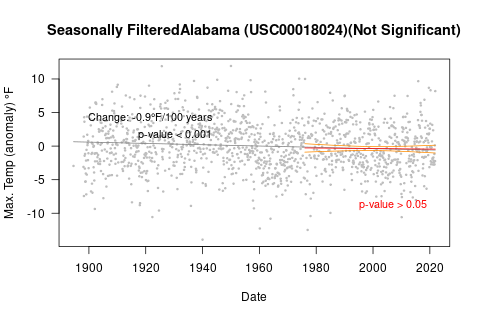
\includegraphics[width=1.00\textwidth]{/home/CAMPUS/mwl04747/github/Climate_Change_Narratives/Social_Media/png/Alabama-USC00018024-GSOM-anomaly.png}
\caption{The changing in monthly temperature data.}
\label{fig:GSOM-anomaly}
\end{figure}

\subsubsection{Method 2: Polynomial Filter}

Project to be followed up with.

\begin{knitrout}
\definecolor{shadecolor}{rgb}{0.969, 0.969, 0.969}\color{fgcolor}\begin{kframe}
\begin{alltt}
\hlcom{# fit polynomial: x^2*b1 + x*b2 + ... + bn}

\hlcom{# create time series object}
\hlcom{#X = [i%365 for i in range(0, len(series))]}
\hlcom{# y = series.values}

\hlcom{# degree = 4}
\hlcom{#coef = polyfit(X, y, degree)}
\hlcom{# print('Coefficients: %s' % coef)}
\hlcom{# create curve}
\end{alltt}
\end{kframe}
\end{knitrout}


\subsection{Extreme Events--Using Daily Records}

\subsubsection{Complicated Nature of Rainfall Patterns}

Rainfall trends are tough. Exteme events can occur in 24 hours or over long periods that might result in floods or droughts. Each region might have different patterns, so developing a consistent approach is tough.

We can look for trends in monthly averages, number of days without rain (important in tropics), and/or extreme events based on daily or hourly data. 

I don't know of a robust way to look at this for the entire globe. 

\begin{knitrout}
\definecolor{shadecolor}{rgb}{0.969, 0.969, 0.969}\color{fgcolor}\begin{kframe}
\begin{alltt}
\hlstd{PRCP.Total} \hlkwb{=} \hlkwd{aggregate}\hlstd{(PRCP}\hlopt{~}\hlstd{Year,} \hlkwc{data}\hlstd{=CHCND, sum,} \hlkwc{na.rm}\hlstd{=T)}
\hlstd{PRCP.Season.Total} \hlkwb{=} \hlkwd{aggregate}\hlstd{(PRCP}\hlopt{~}\hlstd{Season}\hlopt{+}\hlstd{Year,} \hlkwc{data}\hlstd{=CHCND, sum,} \hlkwc{na.rm}\hlstd{=T)}
\end{alltt}
\end{kframe}
\end{knitrout}

Rainfall totals by season might be a useful way to think about changes, because the rainfall is often seasonal, I wonder if we can see pattners by season. 

\begin{knitrout}
\definecolor{shadecolor}{rgb}{0.969, 0.969, 0.969}\color{fgcolor}\begin{kframe}
\begin{alltt}
\hlkwd{ggplot}\hlstd{( )} \hlopt{+}
   \hlkwd{geom_bar}\hlstd{(}\hlkwc{data} \hlstd{= PRCP.Season.Total,}
      \hlkwd{aes}\hlstd{(}\hlkwc{x}\hlstd{=Year,} \hlkwc{y}\hlstd{=PRCP,} \hlkwc{fill}\hlstd{=Season),} \hlkwc{stat}\hlstd{=}\hlstr{"identity"}\hlstd{)} \hlopt{+}
         \hlkwd{xlim}\hlstd{(}\hlkwd{min}\hlstd{(CHCND}\hlopt{$}\hlstd{Year),} \hlkwd{max}\hlstd{(CHCND}\hlopt{$}\hlstd{Year)}\hlopt{-}\hlnum{1}\hlstd{)} \hlopt{+}
   \hlcom{#ylab("Number of Extreme Temps") + # for the y axis label}
   \hlkwd{geom_smooth}\hlstd{(}\hlkwc{data} \hlstd{= PRCP.Total,}
      \hlkwd{aes}\hlstd{(}\hlkwc{y}\hlstd{=PRCP,} \hlkwc{x}\hlstd{=Year),} \hlkwc{method} \hlstd{=} \hlstr{"lm"}\hlstd{,}
      \hlkwc{se} \hlstd{= T,} \hlkwc{color}\hlstd{=} \hlstr{"black"}\hlstd{)}
\end{alltt}


{\ttfamily\noindent\itshape\color{messagecolor}{\#\# `geom\_smooth()` using formula 'y \textasciitilde{} x'}}\end{kframe}
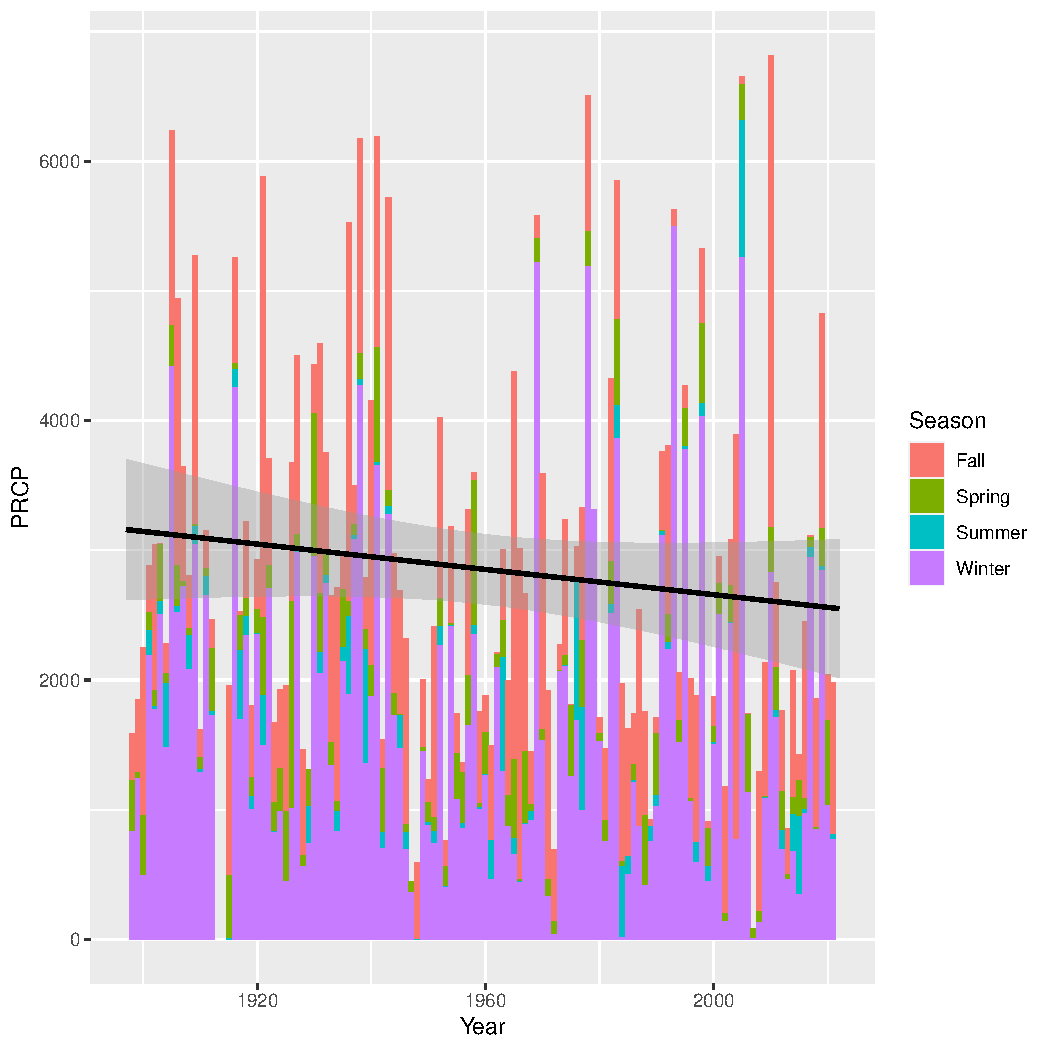
\includegraphics[width=\maxwidth]{figure/unnamed-chunk-9-1} 
\begin{kframe}\begin{alltt}
\hlcom{# + geom_smooth(data= PRCP.Season.Total, aes(x=Year, y = PRCP, color = Season, group=Season), se=F)}
\end{alltt}
\end{kframe}
\end{knitrout}

\subsubsection{Drought}

Days without rain...within a calendar year... bleed over between years isn't captured..

\begin{knitrout}
\definecolor{shadecolor}{rgb}{0.969, 0.969, 0.969}\color{fgcolor}\begin{kframe}
\begin{alltt}
\hlstd{CHCND}\hlopt{$}\hlstd{PRCP.count} \hlkwb{=} \hlkwd{sequence}\hlstd{(}\hlkwd{rle}\hlstd{(CHCND}\hlopt{$}\hlstd{PRCP)}\hlopt{$}\hlstd{lengths)}
\hlstd{Drought.run.temp} \hlkwb{<-} \hlkwd{data.frame}\hlstd{(}\hlkwc{Year} \hlstd{=} \hlnum{NA}\hlstd{,} \hlkwc{lengths}\hlstd{=}\hlnum{NA}\hlstd{,} \hlkwc{values}\hlstd{=}\hlnum{NA}\hlstd{)}
\hlkwa{for}\hlstd{(i} \hlkwa{in} \hlkwd{min}\hlstd{(CHCND}\hlopt{$}\hlstd{Year)}\hlopt{:}\hlkwd{max}\hlstd{(CHCND}\hlopt{$}\hlstd{Year))\{}
   \hlcom{# print(i)}
   \hlstd{run.length} \hlkwb{=} \hlkwd{rle}\hlstd{(CHCND[CHCND}\hlopt{$}\hlstd{Year}\hlopt{==}\hlstd{i,]}\hlopt{$}\hlstd{PRCP)}
   \hlstd{run.length.df} \hlkwb{=} \hlkwd{data.frame}\hlstd{(}\hlkwc{Year} \hlstd{=} \hlkwd{rep}\hlstd{(i,} \hlkwd{length}\hlstd{(run.length}\hlopt{$}\hlstd{values)),}
         \hlkwc{lengths} \hlstd{= run.length}\hlopt{$}\hlstd{lengths,}
         \hlkwc{values} \hlstd{= run.length}\hlopt{$}\hlstd{values)}

   \hlstd{Drought.run.temp} \hlkwb{<-} \hlkwd{rbind}\hlstd{(Drought.run.temp,}
         \hlstd{run.length.df[run.length.df}\hlopt{$}\hlstd{values}\hlopt{==}\hlnum{0}\hlstd{,])}
\hlstd{\}}
\hlstd{Drought.run} \hlkwb{<-} \hlstd{Drought.run.temp[}\hlopt{-}\hlnum{1}\hlstd{,]}
\hlkwd{str}\hlstd{(Drought.run)}
\end{alltt}
\begin{verbatim}
## 'data.frame':	10689 obs. of  3 variables:
##  $ Year   : int  NA NA NA NA NA NA NA NA NA NA ...
##  $ lengths: int  NA NA NA NA NA NA NA NA NA NA ...
##  $ values : int  NA NA NA NA NA NA NA NA NA NA ...
\end{verbatim}
\begin{alltt}
\hlkwd{names}\hlstd{(Drought.run)}
\end{alltt}
\begin{verbatim}
## [1] "Year"    "lengths" "values"
\end{verbatim}
\begin{alltt}
\hlcom{# What is a drought 10 days, 20 days, 40 days?}

\hlstd{Drought.run.10} \hlkwb{=} \hlkwd{aggregate}\hlstd{(lengths}\hlopt{~}\hlstd{Year,}
   \hlkwc{data}\hlstd{=Drought.run[Drought.run}\hlopt{$}\hlstd{lengths}\hlopt{>=}\hlnum{10}\hlstd{,], sum)}
\hlstd{Drought.run.20} \hlkwb{=} \hlkwd{aggregate}\hlstd{(lengths}\hlopt{~}\hlstd{Year,}
   \hlkwc{data}\hlstd{=Drought.run[Drought.run}\hlopt{$}\hlstd{lengths}\hlopt{>=}\hlnum{20}\hlstd{,], sum)}
\hlstd{Drought.run.40} \hlkwb{=} \hlkwd{aggregate}\hlstd{(lengths}\hlopt{~}\hlstd{Year,}
   \hlkwc{data}\hlstd{=Drought.run[Drought.run}\hlopt{$}\hlstd{lengths}\hlopt{>=}\hlnum{40}\hlstd{,], sum)}
\hlstd{Drought.run.100} \hlkwb{=} \hlkwd{aggregate}\hlstd{(lengths}\hlopt{~}\hlstd{Year,}
   \hlkwc{data}\hlstd{=Drought.run[Drought.run}\hlopt{$}\hlstd{lengths}\hlopt{>=}\hlnum{100}\hlstd{,], sum)}
\end{alltt}


{\ttfamily\noindent\bfseries\color{errorcolor}{\#\# Error in aggregate.data.frame(mf[1L], mf[-1L], FUN = FUN, ...): no rows to aggregate}}\begin{alltt}
\hlkwd{plot}\hlstd{(lengths}\hlopt{~}\hlstd{Year, Drought.run.10,} \hlkwc{pch}\hlstd{=}\hlnum{20}\hlstd{,} \hlkwc{cex}\hlstd{=}\hlnum{.5}\hlstd{)}
\hlkwd{points}\hlstd{(lengths}\hlopt{~}\hlstd{Year, Drought.run.20,} \hlkwc{pch}\hlstd{=}\hlnum{20}\hlstd{,} \hlkwc{col}\hlstd{=}\hlstr{"blue"}\hlstd{,} \hlkwc{cex}\hlstd{=}\hlnum{.5}\hlstd{)}
\hlkwd{points}\hlstd{(lengths}\hlopt{~}\hlstd{Year, Drought.run.40,} \hlkwc{pch}\hlstd{=}\hlnum{20}\hlstd{,} \hlkwc{col}\hlstd{=}\hlstr{"red"}\hlstd{,} \hlkwc{cex}\hlstd{=}\hlnum{.5}\hlstd{)}
\hlkwd{points}\hlstd{(lengths}\hlopt{~}\hlstd{Year, Drought.run.100,} \hlkwc{pch}\hlstd{=}\hlnum{20}\hlstd{,} \hlkwc{col}\hlstd{=}\hlstr{"purple"}\hlstd{,} \hlkwc{cex}\hlstd{=}\hlnum{.5}\hlstd{)}
\end{alltt}


{\ttfamily\noindent\bfseries\color{errorcolor}{\#\# Error in eval(m\$data, eframe): object 'Drought.run.100' not found}}\begin{alltt}
\hlkwd{abline}\hlstd{(}\hlkwd{lm}\hlstd{(lengths}\hlopt{~}\hlstd{Year, Drought.run.10))}
\hlkwd{abline}\hlstd{(}\hlkwd{lm}\hlstd{(lengths}\hlopt{~}\hlstd{Year, Drought.run.20),} \hlkwc{col}\hlstd{=}\hlstr{"blue"}\hlstd{)}
\hlkwd{abline}\hlstd{(}\hlkwd{lm}\hlstd{(lengths}\hlopt{~}\hlstd{Year, Drought.run.40),} \hlkwc{col}\hlstd{=}\hlstr{"red"}\hlstd{)}
\end{alltt}
\end{kframe}
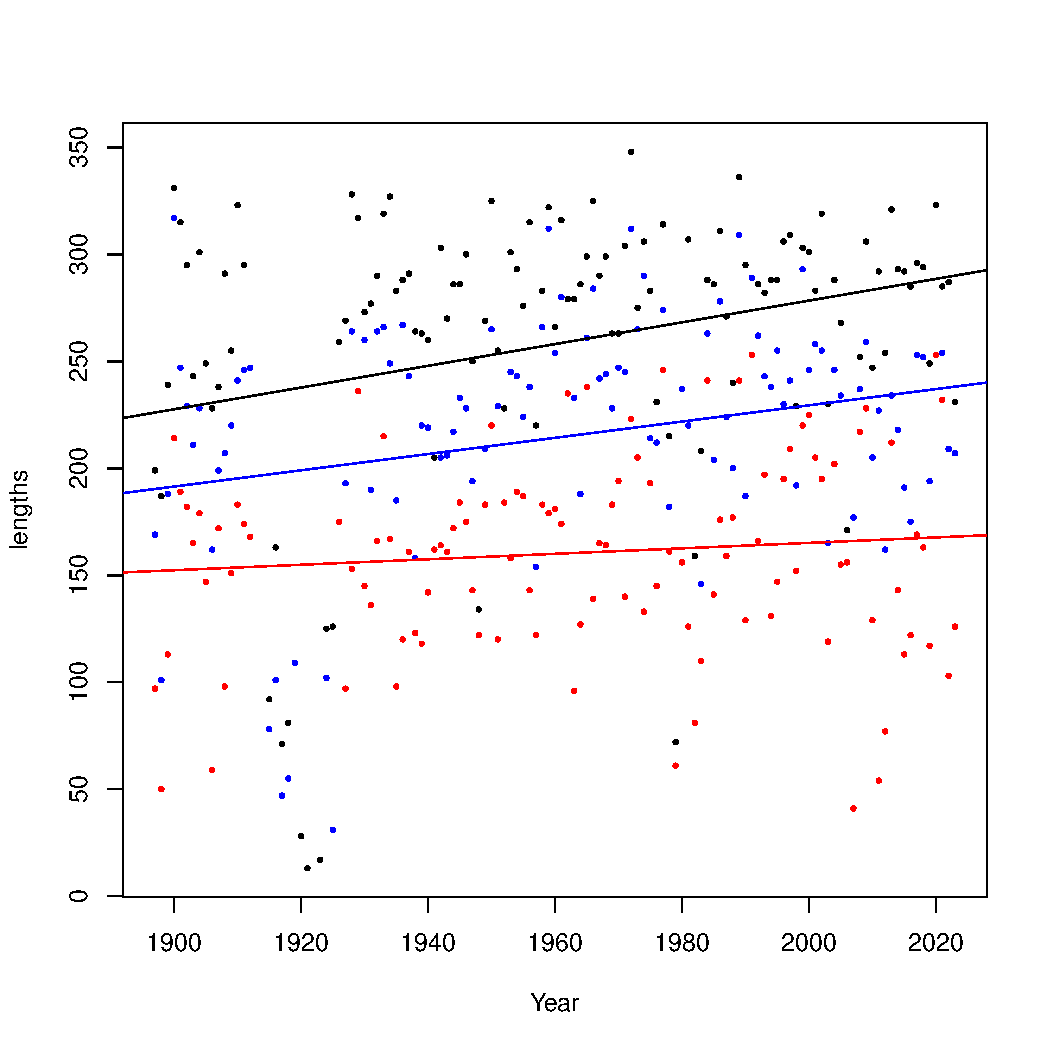
\includegraphics[width=\maxwidth]{figure/unnamed-chunk-10-1} 
\begin{kframe}\begin{alltt}
\hlkwd{abline}\hlstd{(}\hlkwd{lm}\hlstd{(lengths}\hlopt{~}\hlstd{Year, Drought.run.100),} \hlkwc{col}\hlstd{=}\hlstr{"purple"}\hlstd{)}
\end{alltt}


{\ttfamily\noindent\bfseries\color{errorcolor}{\#\# Error in is.data.frame(data): object 'Drought.run.100' not found}}\begin{alltt}
\hlkwd{summary}\hlstd{(}\hlkwd{lm}\hlstd{(lengths}\hlopt{~}\hlstd{Year, Drought.run.100))}
\end{alltt}


{\ttfamily\noindent\bfseries\color{errorcolor}{\#\# Error in is.data.frame(data): object 'Drought.run.100' not found}}\begin{alltt}
\hlkwd{plot}\hlstd{(lengths}\hlopt{~}\hlstd{Year, Drought.run[Drought.run}\hlopt{$}\hlstd{lengths}\hlopt{>}\hlnum{30}\hlstd{,],} \hlkwc{pch}\hlstd{=}\hlnum{20}\hlstd{)}
\hlkwd{plot}\hlstd{(lengths}\hlopt{~}\hlstd{Year, Drought.run[Drought.run}\hlopt{$}\hlstd{lengths}\hlopt{>}\hlnum{30}\hlstd{,],} \hlkwc{pch}\hlstd{=}\hlnum{20}\hlstd{)}


\hlstd{Drought.run.lm} \hlkwb{<-} \hlkwd{lm}\hlstd{(lengths}\hlopt{~}\hlstd{Year, Drought.run[Drought.run}\hlopt{$}\hlstd{lengths}\hlopt{>}\hlnum{10}\hlstd{,])}
\hlkwd{summary}\hlstd{(Drought.run.lm)}
\end{alltt}
\begin{verbatim}
## 
## Call:
## lm(formula = lengths ~ Year, data = Drought.run[Drought.run$lengths > 
##     10, ])
## 
## Residuals:
##    Min     1Q Median     3Q    Max 
## -5.029 -3.489 -1.682  1.520 47.212 
## 
## Coefficients:
##              Estimate Std. Error t value Pr(>|t|)   
## (Intercept) 34.486403  10.929405   3.155  0.00168 **
## Year        -0.009771   0.005589  -1.748  0.08093 . 
## ---
## Signif. codes:  0 '***' 0.001 '**' 0.01 '*' 0.05 '.' 0.1 ' ' 1
## 
## Residual standard error: 5.208 on 628 degrees of freedom
##   (3528 observations deleted due to missingness)
## Multiple R-squared:  0.004842,	Adjusted R-squared:  0.003258 
## F-statistic: 3.056 on 1 and 628 DF,  p-value: 0.08093
\end{verbatim}
\begin{alltt}
\hlkwd{text}\hlstd{(}\hlkwd{min}\hlstd{(Drought.run}\hlopt{$}\hlstd{Year,} \hlkwc{na.rm}\hlstd{=T),} \hlkwd{max}\hlstd{(Drought.run}\hlopt{$}\hlstd{lengths,} \hlkwc{na.rm}\hlstd{=T),}
     \hlkwd{paste}\hlstd{(}\hlstr{"Slope (x100) = "}\hlstd{,} \hlkwd{round}\hlstd{(}\hlkwd{coef}\hlstd{(Drought.run.lm)[}\hlnum{2}\hlstd{]}\hlopt{*}\hlnum{100}\hlstd{,} \hlnum{3}\hlstd{)),} \hlkwc{pos}\hlstd{=}\hlnum{4}\hlstd{)}
\end{alltt}
\end{kframe}
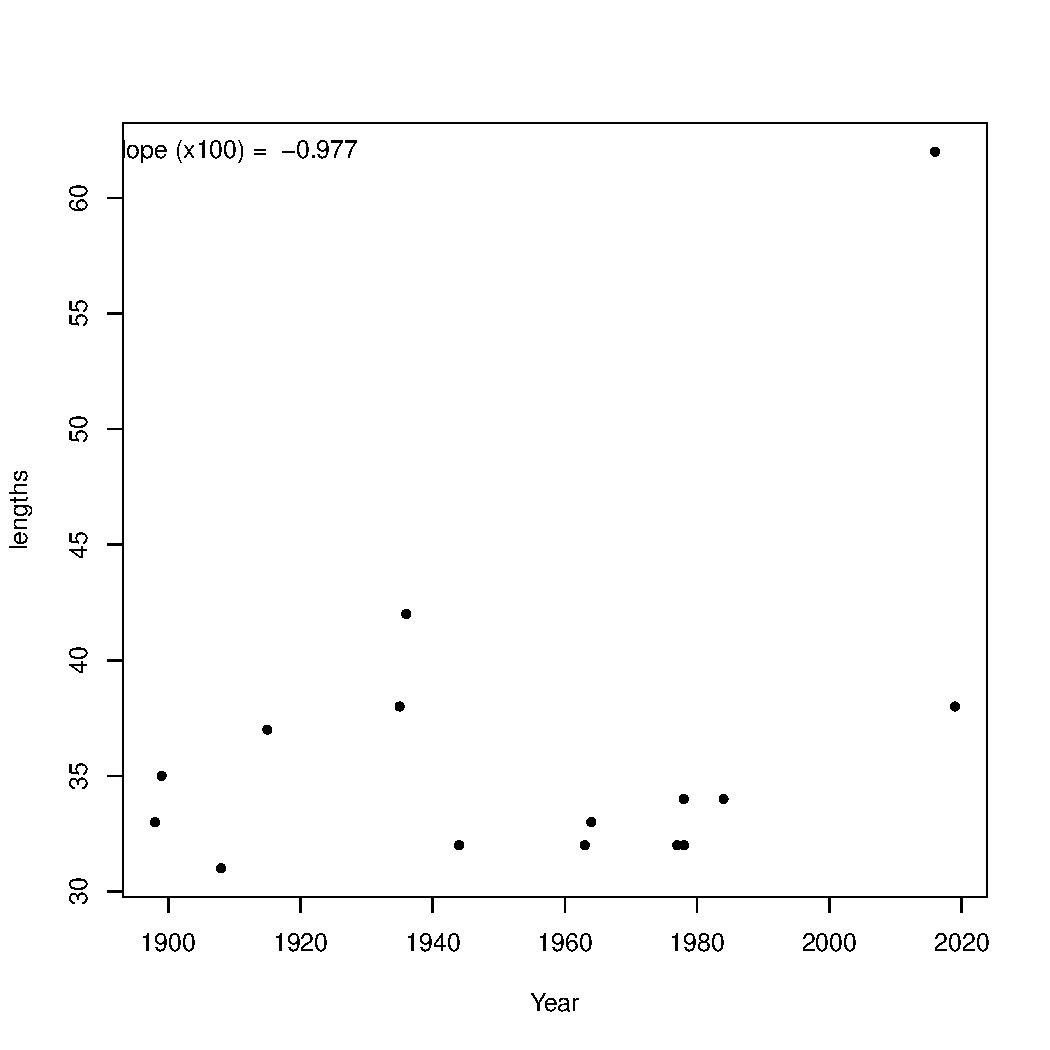
\includegraphics[width=\maxwidth]{figure/unnamed-chunk-10-2} 
\begin{kframe}\begin{alltt}
\hlcom{#plot(PRCP.count ~ Year, data=CHCND[CHCND$PRCP==0,])}
\end{alltt}
\end{kframe}
\end{knitrout}

Rainfall Probability Distributions by decade... to be developed.

\begin{knitrout}
\definecolor{shadecolor}{rgb}{0.969, 0.969, 0.969}\color{fgcolor}\begin{kframe}
\begin{alltt}
\hlstd{CHCND}\hlopt{$}\hlstd{Decade} \hlkwb{<-} \hlkwd{floor_decade}\hlstd{(CHCND}\hlopt{$}\hlstd{Year)}

\hlstd{PRCP.Decade} \hlkwb{<-} \hlkwd{aggregate}\hlstd{(PRCP}\hlopt{~}\hlstd{Month}\hlopt{+}\hlstd{Decade,} \hlkwc{data}\hlstd{=CHCND, sum)}
\hlkwd{head}\hlstd{(PRCP.Decade)}

\hlstd{x} \hlkwb{<-} \hlstd{PRCP.Decade}\hlopt{$}\hlstd{PRCP[PRCP.Decade}\hlopt{$}\hlstd{Decade}\hlopt{==}\hlnum{1900}\hlstd{]}
\hlstd{df} \hlkwb{<-} \hlkwd{approxfun}\hlstd{(}\hlkwd{density}\hlstd{(x))}
\hlkwd{plot}\hlstd{(}\hlnum{1}\hlopt{:}\hlnum{12}\hlstd{,} \hlkwd{density}\hlstd{(x))}
\hlstd{xnew} \hlkwb{<-} \hlkwd{c}\hlstd{(}\hlnum{0.45}\hlstd{,}\hlnum{1.84}\hlstd{,}\hlnum{2.3}\hlstd{)}
\hlkwd{points}\hlstd{(xnew,}\hlkwd{df}\hlstd{(xnew),}\hlkwc{col}\hlstd{=}\hlnum{2}\hlstd{)}
\end{alltt}
\end{kframe}
\end{knitrout}

\begin{knitrout}
\definecolor{shadecolor}{rgb}{0.969, 0.969, 0.969}\color{fgcolor}\begin{kframe}
\begin{alltt}
\hlstd{CHCND}\hlopt{$}\hlstd{Score} \hlkwb{<-} \hlkwd{floor_score}\hlstd{(CHCND}\hlopt{$}\hlstd{Year)}
\end{alltt}
\end{kframe}
\end{knitrout}

\subsection{Record Setting Temperature Records}

In many cases, people seem to "feel" how temperature has been changing over time, and new records seem to capture the attention in the media. So, we'll create a updated record of maximum temperatures and display them. 






This is a common way to communicate temperatures changes. I suspect we have a better sense of change when we notice "extreme" events...

\begin{knitrout}
\definecolor{shadecolor}{rgb}{0.969, 0.969, 0.969}\color{fgcolor}\begin{kframe}
\begin{alltt}
\hlkwd{names}\hlstd{(CHCND)}

\hlstd{minTMIN.length} \hlkwb{=} \hlkwd{aggregate}\hlstd{(minTMIN}\hlopt{~}\hlstd{Year,} \hlkwc{data}\hlstd{=CHCND, length)}
\hlstd{minTMIN.length}\hlopt{$}\hlstd{group} \hlkwb{<-} \hlstr{"Record Lows"}
\hlkwd{names}\hlstd{(minTMIN.length)} \hlkwb{<-} \hlkwd{c}\hlstd{(}\hlstr{"Year"}\hlstd{,} \hlstr{"Num"}\hlstd{,} \hlstr{"Group"}\hlstd{)}
\hlstd{minTMIN.length}\hlopt{$}\hlstd{Num} \hlkwb{=} \hlopt{-}\hlstd{minTMIN.length}\hlopt{$}\hlstd{Num}

\hlstd{maxTMAX.length} \hlkwb{=} \hlkwd{aggregate}\hlstd{(maxTMAX}\hlopt{~}\hlstd{Year,} \hlkwc{data}\hlstd{=CHCND, length);}
\hlstd{maxTMAX.length}\hlopt{$}\hlstd{group} \hlkwb{<-} \hlstr{"Record Highs"}
\hlkwd{names}\hlstd{(maxTMAX.length)} \hlkwb{<-} \hlkwd{c}\hlstd{(}\hlstr{"Year"}\hlstd{,} \hlstr{"Num"}\hlstd{,} \hlstr{"Group"}\hlstd{)}

\hlstd{records} \hlkwb{=} \hlkwd{rbind}\hlstd{(minTMIN.length, maxTMAX.length);} \hlcom{# records}


\hlkwd{ggplot}\hlstd{( )} \hlopt{+}
   \hlkwd{geom_point}\hlstd{(}\hlkwc{data} \hlstd{= CHCND,} \hlkwd{aes}\hlstd{(}\hlkwc{y}\hlstd{=TMIN,} \hlkwc{x}\hlstd{=YearDay),}
      \hlkwc{size}\hlstd{=}\hlnum{.05}\hlstd{,} \hlkwc{color}\hlstd{=}\hlstr{"gray"}\hlstd{)} \hlopt{+}
   \hlkwd{geom_bar}\hlstd{(}\hlkwc{data} \hlstd{= records,} \hlkwd{aes}\hlstd{(}\hlkwc{x}\hlstd{=Year,} \hlkwc{y}\hlstd{=Num,} \hlkwc{fill}\hlstd{=Group),}
      \hlkwc{stat}\hlstd{=}\hlstr{"identity"}\hlstd{,} \hlkwc{position}\hlstd{=}\hlstr{"identity"}\hlstd{)} \hlopt{+}
   \hlkwd{xlim}\hlstd{(}\hlkwd{min}\hlstd{(CHCND}\hlopt{$}\hlstd{Year),} \hlkwd{max}\hlstd{(CHCND}\hlopt{$}\hlstd{Year)}\hlopt{-}\hlnum{1}\hlstd{)} \hlopt{+}
   \hlcom{#ylab("Number of Extreme Temps") + # for the y axis label}
   \hlkwd{scale_fill_manual}\hlstd{(}\hlstr{"Legend"}\hlstd{,}
      \hlkwc{values} \hlstd{=} \hlkwd{c}\hlstd{(}\hlstr{"Record Highs"} \hlstd{=} \hlstr{"red"}\hlstd{,} \hlstr{"Record Lows"} \hlstd{=} \hlstr{"blue"}\hlstd{))} \hlopt{+}
   \hlkwd{geom_smooth}\hlstd{(}\hlkwc{data} \hlstd{= CHCND,} \hlkwd{aes}\hlstd{(}\hlkwc{y}\hlstd{=TMIN,} \hlkwc{x}\hlstd{=YearDay),} \hlkwc{method} \hlstd{=} \hlstr{"lm"}\hlstd{,} \hlkwc{se} \hlstd{=} \hlnum{FALSE}\hlstd{)}
\end{alltt}
\end{kframe}
\end{knitrout}


\begin{knitrout}
\definecolor{shadecolor}{rgb}{0.969, 0.969, 0.969}\color{fgcolor}\begin{kframe}
\begin{alltt}
\hlkwd{ggplot}\hlstd{( )} \hlopt{+}
   \hlkwd{geom_bar}\hlstd{(}\hlkwc{data} \hlstd{= records,} \hlkwd{aes}\hlstd{(}\hlkwc{x}\hlstd{=Year,} \hlkwc{y}\hlstd{=Num,} \hlkwc{fill}\hlstd{=Group),}
      \hlkwc{stat}\hlstd{=}\hlstr{"identity"}\hlstd{,} \hlkwc{position}\hlstd{=}\hlstr{"identity"}\hlstd{)} \hlopt{+}
   \hlkwd{xlim}\hlstd{(}\hlkwd{min}\hlstd{(CHCND}\hlopt{$}\hlstd{Year),} \hlkwd{max}\hlstd{(CHCND}\hlopt{$}\hlstd{Year)}\hlopt{-}\hlnum{1}\hlstd{)} \hlopt{+}
   \hlkwd{ylab}\hlstd{(}\hlstr{"Number of Extreme Temps"}\hlstd{)} \hlopt{+} \hlcom{# for the y axis label}
   \hlkwd{scale_fill_manual}\hlstd{(}\hlstr{"Legend"}\hlstd{,}
      \hlkwc{values} \hlstd{=} \hlkwd{c}\hlstd{(}\hlstr{"Record Highs"} \hlstd{=} \hlstr{"red"}\hlstd{,} \hlstr{"Record Lows"} \hlstd{=} \hlstr{"blue"}\hlstd{))}
\end{alltt}
\end{kframe}
\end{knitrout}

I tried to use a for loop and in then statements and it was painfully slow, so I converted the data to a matrix that can be used by barplots with much more effeciency!

Create the matrix
\begin{knitrout}
\definecolor{shadecolor}{rgb}{0.969, 0.969, 0.969}\color{fgcolor}\begin{kframe}
\begin{alltt}
\hlkwd{library}\hlstd{(lubridate)}
\hlkwd{str}\hlstd{(CHCND)}
\end{alltt}
\begin{verbatim}
## 'data.frame':	49092 obs. of  13 variables:
##  $ Date      : Date, format: "1888-01-01" "1888-01-02" ...
##  $ Year      : num  1888 1888 1888 1888 1888 ...
##  $ yday      : num  1 2 3 4 5 6 7 8 9 10 ...
##  $ TMAX      : num  NA NA NA NA NA NA NA NA NA NA ...
##  $ TMIN      : num  NA NA NA NA NA NA NA NA NA NA ...
##  $ PRCP      : int  NA NA NA NA NA NA NA NA NA NA ...
##  $ YearDay   : num  1888 1888 1888 1888 1888 ...
##  $ mmdd      : chr  "01-01" "01-02" "01-03" "01-04" ...
##  $ Month     : num  1 1 1 1 1 1 1 1 1 1 ...
##  $ Month.name: Factor w/ 12 levels "Jan","Feb","Mar",..: 1 1 1 1 1 1 1 1 1 1 ...
##  $ Season    : chr  "Winter" "Winter" "Winter" "Winter" ...
##  $ PRCP.count: int  1 1 1 1 1 1 1 1 1 1 ...
##  $ Score     : num  1880 1880 1880 1880 1880 1880 1880 1880 1880 1880 ...
\end{verbatim}
\begin{alltt}
\hlstd{TMAX.mat.noleap} \hlkwb{<-} \hlkwd{matrix}\hlstd{(}\hlnum{NA}\hlstd{,} \hlkwc{nrow}\hlstd{=}\hlnum{366}\hlstd{,} \hlkwc{ncol}\hlstd{=}\hlkwd{max}\hlstd{(CHCND}\hlopt{$}\hlstd{Year)} \hlopt{-} \hlkwd{min}\hlstd{(CHCND}\hlopt{$}\hlstd{Year))}
\hlstd{TMIN.mat} \hlkwb{<-} \hlkwd{matrix}\hlstd{(}\hlnum{NA}\hlstd{,} \hlkwc{nrow}\hlstd{=}\hlnum{366}\hlstd{,} \hlkwc{ncol}\hlstd{=}\hlkwd{max}\hlstd{(CHCND}\hlopt{$}\hlstd{Year)} \hlopt{-} \hlkwd{min}\hlstd{(CHCND}\hlopt{$}\hlstd{Year))}
\hlcom{#TMAX.mat.leap <- matrix(NA, nrow=1, ncol=max(CHCND$Year) - min(CHCND$Year))}

\hlcom{# Dumb Method, fraction of year might be better...}

\hlstd{CHCND.noleap} \hlkwb{=} \hlkwd{subset}\hlstd{(CHCND,} \hlkwc{select}\hlstd{=}\hlkwd{c}\hlstd{(Date, Year, yday, TMAX, TMIN, PRCP),}
                      \hlkwc{subset}\hlstd{=(mmdd}\hlopt{!=}\hlstr{"02-29"}\hlstd{))}

\hlcom{## Add yday for leap year }
\hlstd{CHCND.noleap}\hlopt{$}\hlstd{yday[CHCND.noleap}\hlopt{$}\hlstd{yday}\hlopt{>=}\hlnum{60} \hlopt{& !}\hlkwd{leap_year}\hlstd{(CHCND.noleap}\hlopt{$}\hlstd{Date)]}\hlkwb{<-}\hlstd{CHCND.noleap}\hlopt{$}\hlstd{yday[CHCND.noleap}\hlopt{$}\hlstd{yday}\hlopt{>=}\hlnum{60} \hlopt{& !}\hlkwd{leap_year}\hlstd{(CHCND.noleap}\hlopt{$}\hlstd{Date)]} \hlopt{+} \hlnum{1}

\hlcom{## Create leap year dataframe}
\hlstd{CHCND.leap}  \hlkwb{=} \hlkwd{subset}\hlstd{(CHCND,} \hlkwc{select}\hlstd{=}\hlkwd{c}\hlstd{(Date, Year, yday, TMAX, TMIN, PRCP),}
                     \hlkwc{subset}\hlstd{=(mmdd}\hlopt{==}\hlstr{"02-29"}\hlstd{))}
\hlkwd{names}\hlstd{(CHCND.noleap)}
\end{alltt}
\begin{verbatim}
## [1] "Date" "Year" "yday" "TMAX" "TMIN" "PRCP"
\end{verbatim}
\begin{alltt}
\hlstd{years} \hlkwb{=} \hlkwd{seq}\hlstd{(}\hlkwd{min}\hlstd{(CHCND}\hlopt{$}\hlstd{Year),} \hlkwd{max}\hlstd{(CHCND}\hlopt{$}\hlstd{Year),} \hlkwc{by}\hlstd{=}\hlnum{1}\hlstd{)}
\hlstd{year.seq} \hlkwb{=} \hlkwd{data.frame}\hlstd{(}\hlkwc{Year} \hlstd{= years,} \hlkwc{Col} \hlstd{=} \hlkwd{seq_len}\hlstd{(}\hlkwd{length}\hlstd{(}\hlkwd{seq}\hlstd{(}\hlkwd{min}\hlstd{(CHCND}\hlopt{$}\hlstd{Year),} \hlkwd{max}\hlstd{(CHCND}\hlopt{$}\hlstd{Year)))))}

\hlkwa{for}\hlstd{(i} \hlkwa{in} \hlkwd{min}\hlstd{(CHCND.noleap}\hlopt{$}\hlstd{Year)}\hlopt{:}\hlkwd{max}\hlstd{(CHCND.noleap}\hlopt{$}\hlstd{Year))\{}
      \hlkwa{for}\hlstd{(j} \hlkwa{in} \hlkwd{c}\hlstd{(}\hlnum{1}\hlopt{:}\hlnum{59}\hlstd{,} \hlnum{61}\hlopt{:}\hlnum{366}\hlstd{))\{}
      \hlcom{# i=2016; j = 50;}
         \hlstd{TMAX.mat.noleap[j, year.seq}\hlopt{$}\hlstd{Col[year.seq}\hlopt{$}\hlstd{Year}\hlopt{==}\hlstd{i]]} \hlkwb{<-}
         \hlstd{CHCND.noleap}\hlopt{$}\hlstd{TMAX[CHCND.noleap}\hlopt{$}\hlstd{Year}\hlopt{==}\hlstd{i} \hlopt{&} \hlstd{CHCND.noleap}\hlopt{$}\hlstd{yday} \hlopt{==} \hlstd{j]}
         \hlstd{TMIN.mat[j, year.seq}\hlopt{$}\hlstd{Col[year.seq}\hlopt{$}\hlstd{Year}\hlopt{==}\hlstd{i]]} \hlkwb{<-}
         \hlstd{CHCND.noleap}\hlopt{$}\hlstd{TMIN[CHCND.noleap}\hlopt{$}\hlstd{Year}\hlopt{==}\hlstd{i} \hlopt{&} \hlstd{CHCND.noleap}\hlopt{$}\hlstd{yday} \hlopt{==} \hlstd{j]}
      \hlstd{\}}
   \hlkwa{if}\hlstd{(}\hlkwd{leap_year}\hlstd{(i))\{}
      \hlstd{TMAX.mat.noleap[}\hlnum{60}\hlstd{, year.seq}\hlopt{$}\hlstd{Col[year.seq}\hlopt{$}\hlstd{Year}\hlopt{==}\hlstd{i]]} \hlkwb{<-} \hlstd{CHCND.leap}\hlopt{$}\hlstd{TMAX[CHCND.leap}\hlopt{$}\hlstd{Year}\hlopt{==} \hlstd{i} \hlopt{&} \hlstd{CHCND.leap}\hlopt{$}\hlstd{yday} \hlopt{==} \hlnum{60}\hlstd{]}
      \hlstd{TMIN.mat[}\hlnum{60}\hlstd{, year.seq}\hlopt{$}\hlstd{Col[year.seq}\hlopt{$}\hlstd{Year}\hlopt{==}\hlstd{i]]} \hlkwb{<-} \hlstd{CHCND.leap}\hlopt{$}\hlstd{TMIN[CHCND.leap}\hlopt{$}\hlstd{Year}\hlopt{==} \hlstd{i} \hlopt{&} \hlstd{CHCND.leap}\hlopt{$}\hlstd{yday} \hlopt{==} \hlnum{60}\hlstd{]}
      \hlkwd{print}\hlstd{(}\hlkwd{paste0}\hlstd{(}\hlstr{"Added Leap Year"}\hlstd{, i))}
   \hlstd{\}} \hlkwa{else} \hlstd{\{}\hlkwd{print}\hlstd{(}\hlkwd{paste0}\hlstd{(}\hlstr{"Process non-leap year "}\hlstd{, i))\}}
\hlstd{\}}
\end{alltt}
\begin{verbatim}
## [1] "Added Leap Year1888"
## [1] "Process non-leap year 1889"
## [1] "Process non-leap year 1890"
## [1] "Process non-leap year 1891"
## [1] "Added Leap Year1892"
## [1] "Process non-leap year 1893"
## [1] "Process non-leap year 1894"
## [1] "Process non-leap year 1895"
## [1] "Added Leap Year1896"
## [1] "Process non-leap year 1897"
## [1] "Process non-leap year 1898"
## [1] "Process non-leap year 1899"
## [1] "Process non-leap year 1900"
## [1] "Process non-leap year 1901"
## [1] "Process non-leap year 1902"
## [1] "Process non-leap year 1903"
## [1] "Added Leap Year1904"
## [1] "Process non-leap year 1905"
## [1] "Process non-leap year 1906"
## [1] "Process non-leap year 1907"
## [1] "Added Leap Year1908"
## [1] "Process non-leap year 1909"
## [1] "Process non-leap year 1910"
## [1] "Process non-leap year 1911"
## [1] "Added Leap Year1912"
## [1] "Process non-leap year 1913"
## [1] "Process non-leap year 1914"
## [1] "Process non-leap year 1915"
## [1] "Added Leap Year1916"
## [1] "Process non-leap year 1917"
## [1] "Process non-leap year 1918"
## [1] "Process non-leap year 1919"
## [1] "Added Leap Year1920"
## [1] "Process non-leap year 1921"
## [1] "Process non-leap year 1922"
## [1] "Process non-leap year 1923"
## [1] "Added Leap Year1924"
## [1] "Process non-leap year 1925"
## [1] "Process non-leap year 1926"
## [1] "Process non-leap year 1927"
## [1] "Added Leap Year1928"
## [1] "Process non-leap year 1929"
## [1] "Process non-leap year 1930"
## [1] "Process non-leap year 1931"
## [1] "Added Leap Year1932"
## [1] "Process non-leap year 1933"
## [1] "Process non-leap year 1934"
## [1] "Process non-leap year 1935"
## [1] "Added Leap Year1936"
## [1] "Process non-leap year 1937"
## [1] "Process non-leap year 1938"
## [1] "Process non-leap year 1939"
## [1] "Added Leap Year1940"
## [1] "Process non-leap year 1941"
## [1] "Process non-leap year 1942"
## [1] "Process non-leap year 1943"
## [1] "Added Leap Year1944"
## [1] "Process non-leap year 1945"
## [1] "Process non-leap year 1946"
## [1] "Process non-leap year 1947"
## [1] "Added Leap Year1948"
## [1] "Process non-leap year 1949"
## [1] "Process non-leap year 1950"
## [1] "Process non-leap year 1951"
## [1] "Added Leap Year1952"
## [1] "Process non-leap year 1953"
## [1] "Process non-leap year 1954"
## [1] "Process non-leap year 1955"
## [1] "Added Leap Year1956"
## [1] "Process non-leap year 1957"
## [1] "Process non-leap year 1958"
## [1] "Process non-leap year 1959"
## [1] "Added Leap Year1960"
## [1] "Process non-leap year 1961"
## [1] "Process non-leap year 1962"
## [1] "Process non-leap year 1963"
## [1] "Added Leap Year1964"
## [1] "Process non-leap year 1965"
## [1] "Process non-leap year 1966"
## [1] "Process non-leap year 1967"
## [1] "Added Leap Year1968"
## [1] "Process non-leap year 1969"
## [1] "Process non-leap year 1970"
## [1] "Process non-leap year 1971"
## [1] "Added Leap Year1972"
## [1] "Process non-leap year 1973"
## [1] "Process non-leap year 1974"
## [1] "Process non-leap year 1975"
## [1] "Added Leap Year1976"
## [1] "Process non-leap year 1977"
## [1] "Process non-leap year 1978"
## [1] "Process non-leap year 1979"
## [1] "Added Leap Year1980"
## [1] "Process non-leap year 1981"
## [1] "Process non-leap year 1982"
## [1] "Process non-leap year 1983"
## [1] "Added Leap Year1984"
## [1] "Process non-leap year 1985"
## [1] "Process non-leap year 1986"
## [1] "Process non-leap year 1987"
## [1] "Added Leap Year1988"
## [1] "Process non-leap year 1989"
## [1] "Process non-leap year 1990"
## [1] "Process non-leap year 1991"
## [1] "Added Leap Year1992"
## [1] "Process non-leap year 1993"
## [1] "Process non-leap year 1994"
## [1] "Process non-leap year 1995"
## [1] "Added Leap Year1996"
## [1] "Process non-leap year 1997"
## [1] "Process non-leap year 1998"
## [1] "Process non-leap year 1999"
## [1] "Added Leap Year2000"
## [1] "Process non-leap year 2001"
## [1] "Process non-leap year 2002"
## [1] "Process non-leap year 2003"
## [1] "Added Leap Year2004"
## [1] "Process non-leap year 2005"
## [1] "Process non-leap year 2006"
## [1] "Process non-leap year 2007"
## [1] "Added Leap Year2008"
## [1] "Process non-leap year 2009"
## [1] "Process non-leap year 2010"
## [1] "Process non-leap year 2011"
## [1] "Added Leap Year2012"
## [1] "Process non-leap year 2013"
## [1] "Process non-leap year 2014"
## [1] "Process non-leap year 2015"
## [1] "Added Leap Year2016"
## [1] "Process non-leap year 2017"
## [1] "Process non-leap year 2018"
## [1] "Process non-leap year 2019"
## [1] "Added Leap Year2020"
## [1] "Process non-leap year 2021"
\end{verbatim}


{\ttfamily\noindent\bfseries\color{errorcolor}{\#\# Error in `[<-`(`*tmp*`, j, year.seq\$Col[year.seq\$Year == i], value = CHCND.noleap\$TMAX[CHCND.noleap\$Year == : subscript out of bounds}}\begin{alltt}
\hlstd{TMAX.mat.noleap[,}\hlnum{6}\hlstd{]}
\end{alltt}
\begin{verbatim}
##   [1]    NA    NA    NA    NA    NA    NA    NA    NA    NA    NA    NA    NA
##  [13]    NA    NA    NA    NA    NA    NA    NA    NA    NA    NA    NA    NA
##  [25]    NA    NA    NA    NA    NA    NA    NA    NA    NA    NA    NA    NA
##  [37]    NA    NA    NA    NA    NA    NA    NA    NA    NA    NA    NA    NA
##  [49]    NA    NA    NA    NA    NA    NA    NA    NA    NA    NA    NA    NA
##  [61]    NA    NA    NA    NA    NA    NA    NA    NA    NA    NA    NA    NA
##  [73]    NA    NA    NA    NA    NA    NA    NA    NA    NA    NA    NA    NA
##  [85]    NA    NA    NA    NA    NA    NA    NA    NA    NA    NA    NA    NA
##  [97]    NA    NA    NA    NA    NA    NA    NA    NA    NA    NA    NA    NA
## [109]    NA    NA    NA    NA    NA    NA    NA    NA    NA    NA    NA    NA
## [121]    NA    NA    NA    NA    NA    NA    NA    NA    NA    NA    NA    NA
## [133]    NA    NA    NA    NA    NA    NA    NA    NA    NA    NA    NA    NA
## [145]    NA    NA    NA    NA    NA    NA    NA    NA    NA    NA    NA    NA
## [157]    NA    NA    NA    NA    NA    NA    NA    NA    NA    NA    NA    NA
## [169]    NA    NA    NA    NA    NA    NA    NA    NA    NA    NA    NA    NA
## [181]    NA    NA    NA    NA    NA    NA    NA    NA    NA    NA    NA    NA
## [193]    NA    NA    NA    NA    NA    NA    NA    NA    NA    NA    NA    NA
## [205]    NA    NA    NA    NA    NA    NA    NA    NA    NA    NA    NA    NA
## [217]    NA    NA    NA    NA    NA    NA    NA    NA    NA    NA    NA    NA
## [229]    NA    NA    NA    NA    NA    NA    NA    NA    NA    NA    NA    NA
## [241]    NA    NA    NA    NA 89.96 86.00 86.00 87.08 78.98 86.00 86.00 86.00
## [253] 80.96 80.06 78.98 78.98 82.04 86.00 86.00 89.06 84.92 87.08 84.02 84.92
## [265] 87.98 86.00 86.00 84.92 84.02 82.94 78.08 77.00 75.92 78.08 84.02 80.96
## [277] 80.06 80.96 77.00 82.04 77.00 75.92 82.04 84.92 80.96 80.06 78.98 68.00
## [289] 64.94 68.00 66.92 66.02 73.04 78.08 78.98 71.96 78.98 78.98 82.04 80.06
## [301] 80.06 71.06 59.00 60.08 62.96 68.00 73.94 77.00 75.02 59.00 62.06 62.06
## [313] 62.96 66.92 64.94 66.02 69.08 69.08 69.98 69.98 57.02 71.06 71.96 64.04
## [325] 53.96 69.08 68.00 50.00 42.08 44.96 51.08 57.02 59.00 68.00 64.04 55.94
## [337] 60.08 62.06 32.00 46.94 51.98 53.96 57.92 57.92 57.92 62.96 66.02 60.98
## [349] 57.92 66.02 66.02 42.08 50.00 55.04 46.94 51.98 57.92 66.92 68.00 66.02
## [361] 66.02 57.92 62.06 60.98 64.04 42.08
\end{verbatim}
\begin{alltt}
\hlstd{TMAX.mat.noleap[,}\hlnum{7}\hlstd{]}
\end{alltt}
\begin{verbatim}
##   [1]    NA    NA    NA    NA    NA    NA    NA    NA    NA    NA    NA    NA
##  [13]    NA    NA    NA    NA    NA    NA    NA    NA    NA    NA    NA    NA
##  [25]    NA    NA    NA    NA    NA    NA    NA 62.06 55.04 71.96 39.92 44.96
##  [37] 55.04 62.96 68.00 73.04 60.98 53.96 60.08 50.00 50.00 37.04 42.98 57.92
##  [49] 69.98 66.02 66.92 62.96 50.00 35.96 35.96 35.06 42.08 59.00 55.04    NA
##  [61] 64.94 69.08 73.04 73.04 73.04 62.96 69.98 73.94 73.04 78.98 78.08 66.92
##  [73] 75.02 80.06 78.08 78.98 80.06 82.94 84.02 75.92 84.02 86.00 68.00 68.00
##  [85] 46.94 35.06 42.98 59.00 51.98 59.00 73.94 66.92 64.94 73.94 71.06 71.06
##  [97] 66.92 75.02 75.02 82.04 62.96 73.04 64.94 68.00 77.00 73.04 84.92 89.96
## [109] 89.06 82.94 73.04 73.94 71.06 71.96 75.02 78.98 82.04 84.92 87.08 89.06
## [121] 82.94 86.00 86.00 84.92 89.06 87.98 87.98 91.94 86.00 93.92 93.02 87.08
## [133] 87.08 86.00 87.08 84.02 89.06 89.96 84.02 64.04 60.98 64.94 75.92 71.06
## [145] 75.92 78.08 80.06 82.04 84.92 82.94 78.08 75.92 73.04 82.94 87.98 91.04
## [157] 91.94 78.08 84.02 91.04 93.92 93.02 91.94 91.94 96.08 98.06 91.94 93.02
## [169] 91.94 86.00 89.06 89.96 95.00 89.96 91.94 89.96 84.92 93.92 95.00 96.98
## [181] 98.06 96.98 93.92 93.92 93.92 98.06 93.92 80.06 89.06 89.06 75.02 77.00
## [193] 84.92 89.06 89.96 89.96 91.04 86.00 89.06 87.98 89.06 89.96 87.08 87.08
## [205] 87.98 87.08 89.96 89.06 87.08 91.94 89.06 89.06 91.04 91.94 87.98 89.96
## [217] 89.06 75.02 78.08 82.94 89.96 93.02 95.00 96.08 93.92 98.06 98.96 98.96
## [229] 89.96 86.00 89.06 89.06 89.06 87.98 75.02 71.06 82.94 84.92 87.98 86.00
## [241] 86.00 84.02 87.08 87.98    NA    NA    NA    NA    NA    NA    NA    NA
## [253]    NA    NA    NA    NA    NA    NA    NA    NA    NA    NA    NA    NA
## [265]    NA    NA    NA    NA    NA    NA    NA    NA    NA    NA    NA    NA
## [277]    NA    NA    NA    NA    NA    NA    NA    NA    NA    NA    NA    NA
## [289]    NA    NA    NA    NA    NA    NA    NA    NA    NA    NA    NA    NA
## [301]    NA    NA    NA    NA    NA    NA    NA    NA    NA    NA    NA    NA
## [313]    NA    NA    NA    NA    NA    NA    NA    NA    NA    NA    NA    NA
## [325]    NA    NA    NA    NA    NA    NA    NA    NA    NA    NA    NA    NA
## [337]    NA    NA    NA    NA    NA    NA    NA    NA    NA    NA    NA    NA
## [349]    NA    NA    NA    NA    NA    NA    NA    NA    NA    NA    NA    NA
## [361]    NA    NA    NA    NA    NA    NA
\end{verbatim}
\begin{alltt}
\hlstd{TMAX.mat.noleap[}\hlnum{60}\hlopt{:}\hlnum{61}\hlstd{,}\hlnum{120}\hlopt{:}\hlnum{134}\hlstd{]}
\end{alltt}
\begin{verbatim}
##      [,1]  [,2]  [,3]  [,4]  [,5]  [,6]  [,7]  [,8]  [,9] [,10] [,11] [,12]
## [1,]   NA 51.98    NA    NA    NA 64.04    NA    NA    NA 69.08    NA    NA
## [2,]   77 62.06 62.06 51.08 78.98 73.04 48.92 48.92 55.04 71.96 71.06 71.06
##      [,13] [,14] [,15]
## [1,]    NA 57.02    NA
## [2,] 66.92 64.94 80.96
\end{verbatim}
\begin{alltt}
\hlstd{TMIN.mat[}\hlnum{60}\hlopt{:}\hlnum{61}\hlstd{,}\hlnum{120}\hlopt{:}\hlnum{134}\hlstd{]}
\end{alltt}
\begin{verbatim}
##       [,1]  [,2]  [,3]  [,4]  [,5]  [,6]  [,7]  [,8]  [,9] [,10] [,11] [,12]
## [1,]    NA 19.04    NA    NA    NA 53.06    NA    NA    NA 28.94    NA    NA
## [2,] 33.08 32.00 30.92 24.08 44.96 62.06 33.08 19.94 51.98 44.96 53.06 55.94
##      [,13] [,14] [,15]
## [1,]    NA 24.98    NA
## [2,] 57.92 42.08 57.02
\end{verbatim}
\end{kframe}
\end{knitrout}


\begin{knitrout}
\definecolor{shadecolor}{rgb}{0.969, 0.969, 0.969}\color{fgcolor}\begin{kframe}
\begin{alltt}
\hlkwd{setwd}\hlstd{(}\hlstr{"/home/CAMPUS/mwl04747/github/Climate_Change_Narratives/"}\hlstd{)}
\hlkwd{png}\hlstd{(}\hlkwd{paste0}\hlstd{(}\hlstr{"Social_Media//png//"}\hlstd{, fips}\hlopt{$}\hlstd{State,} \hlstr{"-"}\hlstd{, stid,} \hlstr{"-CHCND_Records.png"}\hlstd{),} \hlkwc{width} \hlstd{=} \hlnum{480}\hlstd{,} \hlkwc{height} \hlstd{=} \hlnum{280}\hlstd{,} \hlkwc{units} \hlstd{=} \hlstr{"px"}\hlstd{,} \hlkwc{pointsize} \hlstd{=} \hlnum{12}\hlstd{,} \hlkwc{bg} \hlstd{=} \hlstr{"white"}\hlstd{)}

\hlstd{results}\hlkwb{<-}\hlkwa{NULL}
\hlstd{decades} \hlkwb{<-} \hlstd{years[years}\hlopt{/}\hlnum{10} \hlopt{==} \hlkwd{floor}\hlstd{(years}\hlopt{/}\hlnum{10}\hlstd{)]}
\hlstd{i} \hlkwb{=} \hlkwd{max}\hlstd{(CHCND}\hlopt{$}\hlstd{Year)}
\hlcom{# START LOOP}
   \hlstd{j} \hlkwb{=} \hlkwd{which}\hlstd{(years} \hlopt \hlstd{i)}
   \hlkwa{if}\hlstd{(}\hlkwd{sum}\hlstd{(}\hlkwd{is.na}\hlstd{(TMAX.mat.noleap[,j]))}\hlopt{==}\hlnum{366}\hlstd{)} \hlkwa{next}
\end{alltt}


{\ttfamily\noindent\bfseries\color{errorcolor}{\#\# Error in TMAX.mat.noleap[, j]: subscript out of bounds}}\begin{alltt}
\hlstd{TMAX1} \hlkwb{=} \hlkwd{apply}\hlstd{(TMAX.mat.noleap[,}\hlnum{1}\hlopt{:}\hlstd{j],} \hlnum{1}\hlstd{,} \hlkwa{function} \hlstd{(}\hlkwc{x}\hlstd{)} \hlkwd{which.max}\hlstd{(x));}
\end{alltt}


{\ttfamily\noindent\bfseries\color{errorcolor}{\#\# Error in TMAX.mat.noleap[, 1:j]: subscript out of bounds}}\begin{alltt}
\hlkwd{is.na}\hlstd{(TMAX1)} \hlkwb{<-} \hlkwd{lengths}\hlstd{(TMAX1)} \hlopt{==} \hlnum{0}
\end{alltt}


{\ttfamily\noindent\bfseries\color{errorcolor}{\#\# Error in lengths(TMAX1): object 'TMAX1' not found}}\begin{alltt}
\hlstd{TMAX1} \hlkwb{<-} \hlkwd{unlist}\hlstd{(TMAX1)}
\end{alltt}


{\ttfamily\noindent\bfseries\color{errorcolor}{\#\# Error in unlist(TMAX1): object 'TMAX1' not found}}\begin{alltt}
\hlstd{TMAX1} \hlkwb{<-} \hlkwd{count}\hlstd{(TMAX1)}
\end{alltt}


{\ttfamily\noindent\bfseries\color{errorcolor}{\#\# Error in count(TMAX1): object 'TMAX1' not found}}\begin{alltt}
\hlcom{#str(TMAX1)}
\hlkwd{names}\hlstd{(TMAX1)}\hlkwb{=}\hlkwd{c}\hlstd{(}\hlstr{"Year"}\hlstd{,} \hlstr{"TMAX"}\hlstd{)}
\end{alltt}


{\ttfamily\noindent\bfseries\color{errorcolor}{\#\# Error in names(TMAX1) = c("{}Year"{}, "{}TMAX"{}): object 'TMAX1' not found}}\begin{alltt}
\hlstd{TMAX_na} \hlkwb{=} \hlkwd{data.frame}\hlstd{(}\hlkwc{Year}\hlstd{=}\hlnum{1}\hlopt{:}\hlstd{j)}
\hlstd{TMAX} \hlkwb{<-} \hlkwd{merge}\hlstd{(TMAX_na, TMAX1,} \hlkwc{all.x}\hlstd{=}\hlnum{TRUE}\hlstd{,} \hlkwc{by}\hlstd{=}\hlstr{"Year"}\hlstd{)}
\end{alltt}


{\ttfamily\noindent\bfseries\color{errorcolor}{\#\# Error in merge(TMAX\_na, TMAX1, all.x = TRUE, by = "{}Year"{}): object 'TMAX1' not found}}\begin{alltt}
\hlkwa{if}\hlstd{(}\hlkwd{sum}\hlstd{(}\hlkwd{is.na}\hlstd{(TMIN.mat[,j]))}\hlopt{==}\hlnum{366}\hlstd{)} \hlkwa{next}
\end{alltt}


{\ttfamily\noindent\bfseries\color{errorcolor}{\#\# Error in TMIN.mat[, j]: subscript out of bounds}}\begin{alltt}
   \hlcom{# Select Minimum and Change to Negative Value}
\hlstd{TMIN1} \hlkwb{=} \hlkwd{apply}\hlstd{(TMIN.mat[,}\hlnum{1}\hlopt{:}\hlstd{j],} \hlnum{1}\hlstd{,} \hlkwa{function} \hlstd{(}\hlkwc{x}\hlstd{)} \hlkwd{which.min}\hlstd{(x));}
\end{alltt}


{\ttfamily\noindent\bfseries\color{errorcolor}{\#\# Error in TMIN.mat[, 1:j]: subscript out of bounds}}\begin{alltt}
\hlkwd{is.na}\hlstd{(TMIN1)} \hlkwb{<-} \hlkwd{lengths}\hlstd{(TMIN1)} \hlopt{==} \hlnum{0}
\end{alltt}


{\ttfamily\noindent\bfseries\color{errorcolor}{\#\# Error in lengths(TMIN1): object 'TMIN1' not found}}\begin{alltt}
\hlstd{TMIN1} \hlkwb{<-} \hlkwd{unlist}\hlstd{(TMIN1)}
\end{alltt}


{\ttfamily\noindent\bfseries\color{errorcolor}{\#\# Error in unlist(TMIN1): object 'TMIN1' not found}}\begin{alltt}
\hlstd{TMIN1} \hlkwb{<-} \hlkwd{count}\hlstd{(TMIN1)} \hlcom{# Max Counts Negagive}
\end{alltt}


{\ttfamily\noindent\bfseries\color{errorcolor}{\#\# Error in count(TMIN1): object 'TMIN1' not found}}\begin{alltt}
\hlcom{#str(TMIN1)   }
\hlkwd{names}\hlstd{(TMIN1)}\hlkwb{=}\hlkwd{c}\hlstd{(}\hlstr{"Year"}\hlstd{,} \hlstr{"TMIN"}\hlstd{)}
\end{alltt}


{\ttfamily\noindent\bfseries\color{errorcolor}{\#\# Error in names(TMIN1) = c("{}Year"{}, "{}TMIN"{}): object 'TMIN1' not found}}\begin{alltt}
\hlstd{TMIN_na} \hlkwb{<-} \hlkwd{data.frame}\hlstd{(}\hlkwc{Year}\hlstd{=}\hlnum{1}\hlopt{:}\hlstd{j)}
\hlstd{TMIN} \hlkwb{<-} \hlkwd{merge}\hlstd{(TMIN_na, TMIN1,} \hlkwc{all.x}\hlstd{=}\hlnum{TRUE}\hlstd{,} \hlkwc{by}\hlstd{=}\hlstr{"Year"}\hlstd{)}
\end{alltt}


{\ttfamily\noindent\bfseries\color{errorcolor}{\#\# Error in merge(TMIN\_na, TMIN1, all.x = TRUE, by = "{}Year"{}): object 'TMIN1' not found}}\begin{alltt}
\hlstd{R1} \hlkwb{<-} \hlkwd{merge}\hlstd{(TMAX, TMIN,} \hlkwc{by}\hlstd{=}\hlstr{"Year"}\hlstd{)}
\end{alltt}


{\ttfamily\noindent\bfseries\color{errorcolor}{\#\# Error in merge(TMAX, TMIN, by = "{}Year"{}): object 'TMAX' not found}}\begin{alltt}
\hlstd{R1}\hlopt{$}\hlstd{Index} \hlkwb{=} \hlkwd{rep}\hlstd{(j,} \hlkwd{nrow}\hlstd{(R1))}
\end{alltt}


{\ttfamily\noindent\bfseries\color{errorcolor}{\#\# Error in nrow(R1): object 'R1' not found}}\begin{alltt}
\hlcom{#results = rbind(results, R)}
\hlstd{R1}\hlopt{$}\hlstd{TMIN} \hlkwb{=} \hlopt{-}\hlstd{R1}\hlopt{$}\hlstd{TMIN}
\end{alltt}


{\ttfamily\noindent\bfseries\color{errorcolor}{\#\# Error in eval(expr, envir, enclos): object 'R1' not found}}\begin{alltt}
\hlcom{## Sorting out X Axis}
\hlstd{tic.no} \hlkwb{<-} \hlnum{4}
\hlstd{rowskip} \hlkwb{=} \hlkwd{round}\hlstd{(}\hlkwd{nrow}\hlstd{(R1)}\hlopt{/}\hlstd{tic.no,} \hlnum{0}\hlstd{)}
\end{alltt}


{\ttfamily\noindent\bfseries\color{errorcolor}{\#\# Error in nrow(R1): object 'R1' not found}}\begin{alltt}
\hlstd{row_numb} \hlkwb{<-} \hlkwd{seq_len}\hlstd{(}\hlkwd{nrow}\hlstd{(R1))} \hlopt \hlstd{rowskip}
\end{alltt}


{\ttfamily\noindent\bfseries\color{errorcolor}{\#\# Error in nrow(R1): object 'R1' not found}}\begin{alltt}
\hlstd{row.sel} \hlkwb{=} \hlkwd{which}\hlstd{(row_numb} \hlopt \hlkwd{c}\hlstd{(}\hlnum{1}\hlstd{))}
\end{alltt}


{\ttfamily\noindent\bfseries\color{errorcolor}{\#\# Error in row\_numb \%in\% c(1): object 'row\_numb' not found}}\begin{alltt}
\hlstd{index.year} \hlkwb{<-} \hlstd{years[row.sel]}
\end{alltt}


{\ttfamily\noindent\bfseries\color{errorcolor}{\#\# Error in eval(expr, envir, enclos): object 'row.sel' not found}}\begin{alltt}
\hlcom{# switch to decades?}

\hlstd{xtics} \hlkwb{=} \hlstd{row.sel}
\end{alltt}


{\ttfamily\noindent\bfseries\color{errorcolor}{\#\# Error in eval(expr, envir, enclos): object 'row.sel' not found}}\begin{alltt}
\hlstd{xlabs} \hlkwb{=} \hlstd{index.year}
\end{alltt}


{\ttfamily\noindent\bfseries\color{errorcolor}{\#\# Error in eval(expr, envir, enclos): object 'index.year' not found}}\begin{alltt}
\hlstd{yrange} \hlkwb{=} \hlkwd{range}\hlstd{(}\hlkwd{c}\hlstd{(R1}\hlopt{$}\hlstd{TMIN, R1}\hlopt{$}\hlstd{TMAX),} \hlkwc{na.rm}\hlstd{=T)}
\end{alltt}


{\ttfamily\noindent\bfseries\color{errorcolor}{\#\# Error in eval(expr, envir, enclos): object 'R1' not found}}\begin{alltt}
\hlstd{ytics} \hlkwb{=} \hlkwd{floor}\hlstd{(}\hlkwd{seq}\hlstd{(yrange[}\hlnum{1}\hlstd{], yrange[}\hlnum{2}\hlstd{],} \hlkwc{length.out}\hlstd{=tic.no))}
\end{alltt}


{\ttfamily\noindent\bfseries\color{errorcolor}{\#\# Error in seq(yrange[1], yrange[2], length.out = tic.no): object 'yrange' not found}}\begin{alltt}
\hlstd{ylabs} \hlkwb{=} \hlkwd{as.character}\hlstd{(}\hlkwd{abs}\hlstd{(ytics))}
\end{alltt}


{\ttfamily\noindent\bfseries\color{errorcolor}{\#\# Error in eval(expr, envir, enclos): object 'ytics' not found}}\begin{alltt}
\hlkwd{par}\hlstd{(}\hlkwc{las}\hlstd{=}\hlnum{1}\hlstd{,} \hlkwc{xpd}\hlstd{=}\hlnum{TRUE}\hlstd{)}
\hlkwd{plot}\hlstd{(}\hlkwd{c}\hlstd{(}\hlnum{1}\hlstd{,}\hlkwd{nrow}\hlstd{(R1)),} \hlkwd{c}\hlstd{(yrange[}\hlnum{1}\hlstd{], yrange[}\hlnum{2}\hlstd{]),} \hlkwc{ty}\hlstd{=}\hlstr{"n"}\hlstd{,} \hlkwc{xaxt}\hlstd{=}\hlstr{'n'}\hlstd{,} \hlkwc{yaxt}\hlstd{=}\hlstr{'n'}\hlstd{,} \hlkwc{xlab}\hlstd{=}\hlstr{"Year"}\hlstd{,} \hlkwc{ylab}\hlstd{=}\hlstr{"No. of Record Temps"}\hlstd{,} \hlkwc{main}\hlstd{=}\hlstr{"Record Highs and Lows"}\hlstd{)}
\end{alltt}


{\ttfamily\noindent\bfseries\color{errorcolor}{\#\# Error in nrow(R1): object 'R1' not found}}\begin{alltt}
\hlkwd{axis}\hlstd{(}\hlnum{2}\hlstd{,}\hlkwc{at}\hlstd{=ytics,} \hlkwc{labels}\hlstd{=ylabs)}
\end{alltt}


{\ttfamily\noindent\bfseries\color{errorcolor}{\#\# Error in axis(2, at = ytics, labels = ylabs): object 'ytics' not found}}\begin{alltt}
\hlkwd{axis}\hlstd{(}\hlnum{1}\hlstd{,}\hlkwc{at}\hlstd{=xtics,} \hlkwc{labels}\hlstd{=xlabs)}
\end{alltt}


{\ttfamily\noindent\bfseries\color{errorcolor}{\#\# Error in axis(1, at = xtics, labels = xlabs): object 'xtics' not found}}\begin{alltt}
\hlkwd{barplot}\hlstd{(}\hlkwc{height} \hlstd{= R1}\hlopt{$}\hlstd{TMAX,} \hlkwc{space}\hlstd{=}\hlnum{0}\hlstd{,} \hlkwc{add} \hlstd{=} \hlnum{TRUE}\hlstd{,} \hlkwc{axes} \hlstd{=} \hlnum{FALSE}\hlstd{,} \hlkwc{col}\hlstd{=}\hlstr{"red"}\hlstd{)}
\end{alltt}


{\ttfamily\noindent\bfseries\color{errorcolor}{\#\# Error in barplot(height = R1\$TMAX, space = 0, add = TRUE, axes = FALSE, : object 'R1' not found}}\begin{alltt}
\hlkwd{barplot}\hlstd{(}\hlkwc{height} \hlstd{= R1}\hlopt{$}\hlstd{TMIN,} \hlkwc{space}\hlstd{=}\hlnum{0}\hlstd{,} \hlkwc{add} \hlstd{=} \hlnum{TRUE}\hlstd{,} \hlkwc{axes} \hlstd{=} \hlnum{FALSE}\hlstd{,} \hlkwc{col}\hlstd{=}\hlstr{"blue"}\hlstd{)}
\end{alltt}


{\ttfamily\noindent\bfseries\color{errorcolor}{\#\# Error in barplot(height = R1\$TMIN, space = 0, add = TRUE, axes = FALSE, : object 'R1' not found}}\begin{alltt}
\hlcom{# END LOOP}

\hlkwd{dev.off}\hlstd{()}
\end{alltt}
\begin{verbatim}
## pdf 
##   2
\end{verbatim}
\end{kframe}
\end{knitrout}

The patterns of record temperatures often shows increasing number of new high temperature records  and fewer record low temperatures more recently, but as usual, it depends on the location (Figure~\ref{fig:Records}).
\begin{figure}
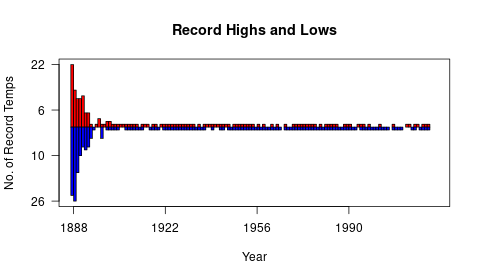
\includegraphics[width=1.00\textwidth]{/home/CAMPUS/mwl04747/github/Climate_Change_Narratives/Social_Media/png/Alabama-USC00018024-CHCND_Records.png}
\caption{Daily temperatures that have been the highest on record (in red) and lowest on record (in blue). In some cases, climate change has created more records in the recent decades, while other stations seem don't show that trend.}
\label{fig:Records}
\end{figure}

\subsection{Iterate TMAX vs. Month Boxplots}

Evaluating the changes in TMAX and Monthly temperatures might be useful, but for now, I think it's hard to see the patterns. 



begin{figure}
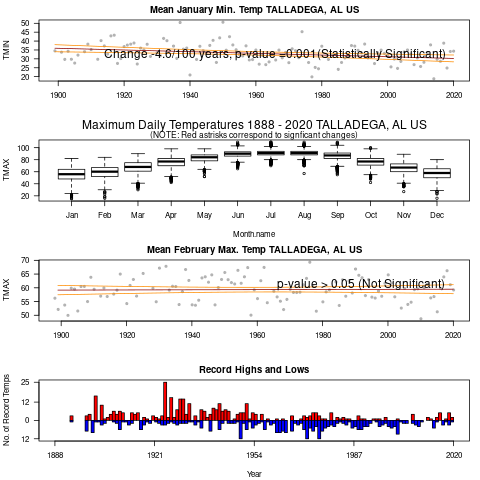
\includegraphics[width=1.00\textwidth]{/home/CAMPUS/mwl04747/github/Climate_Change_Narratives/Social_Media/png/Alabama-USC00018024-GSOM.png}
\caption{Climate can be analyzed using several types of lenses. In this case, we have analyzed show the months with the greatest changes. The first figure is monthly average of TMINs (daily low temperatures) with a best fit line. The second figure shows the monthly TMAX range and asterisks indicate singificant changes over the station record and the third figure is the trend for these TMAXs over time and includes the best fit line. The final figure shows the daily temperatures that have been the highest on record (in red). In some cases, climate change has created more records in the recent decades, while other stations seem don't show that trend.}
\label{fig:GSOM}
\end{figure}

\subsection{Four Plots Compelling Figures}

To test the code, I have created graphics that can then be used in the animation process, i.e. try to create code that doesn't get too complicated and then fail! 

\begin{knitrout}
\definecolor{shadecolor}{rgb}{0.969, 0.969, 0.969}\color{fgcolor}\begin{kframe}


{\ttfamily\noindent\bfseries\color{errorcolor}{\#\# Error in paste0(png\_public, panel4.png): object 'png\_public' not found}}\end{kframe}
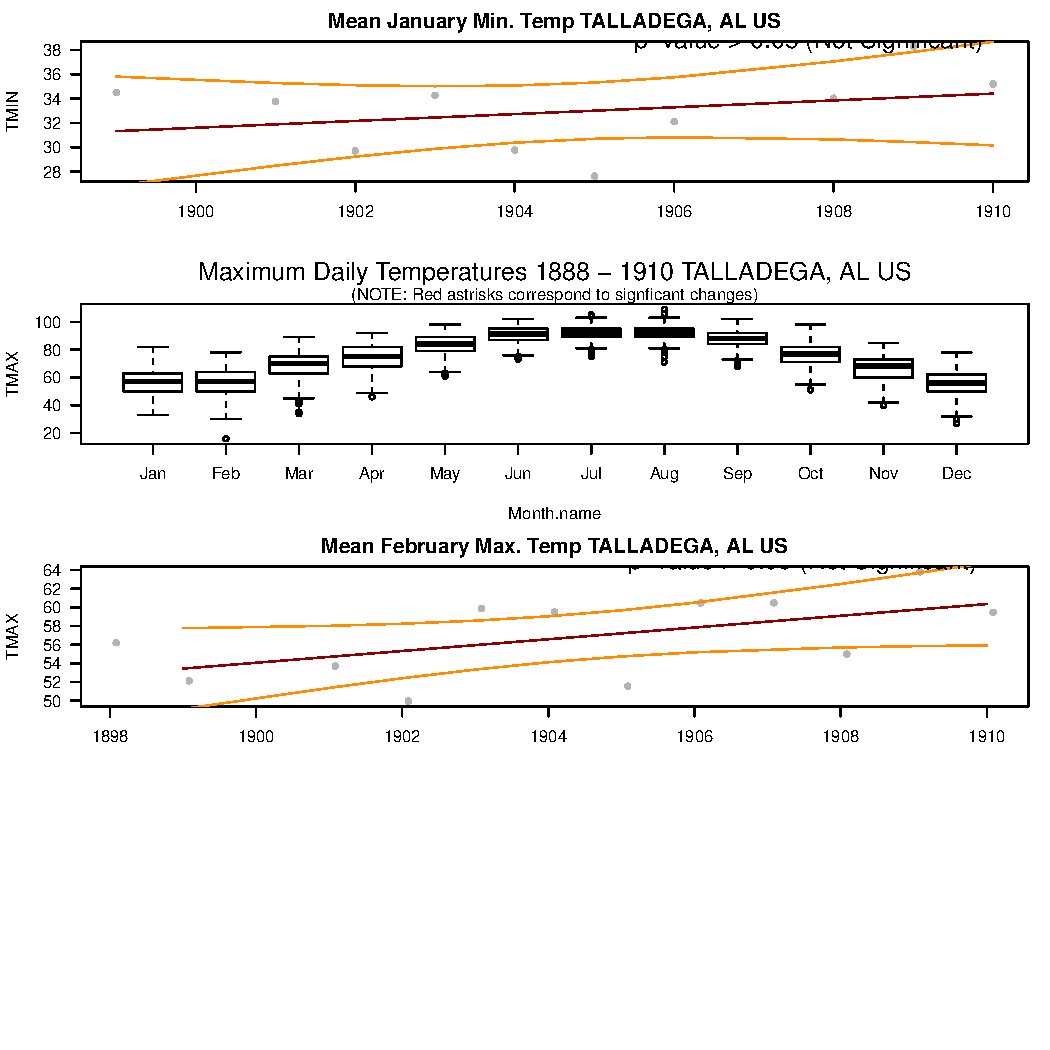
\includegraphics[width=\maxwidth]{figure/static_template-1} 

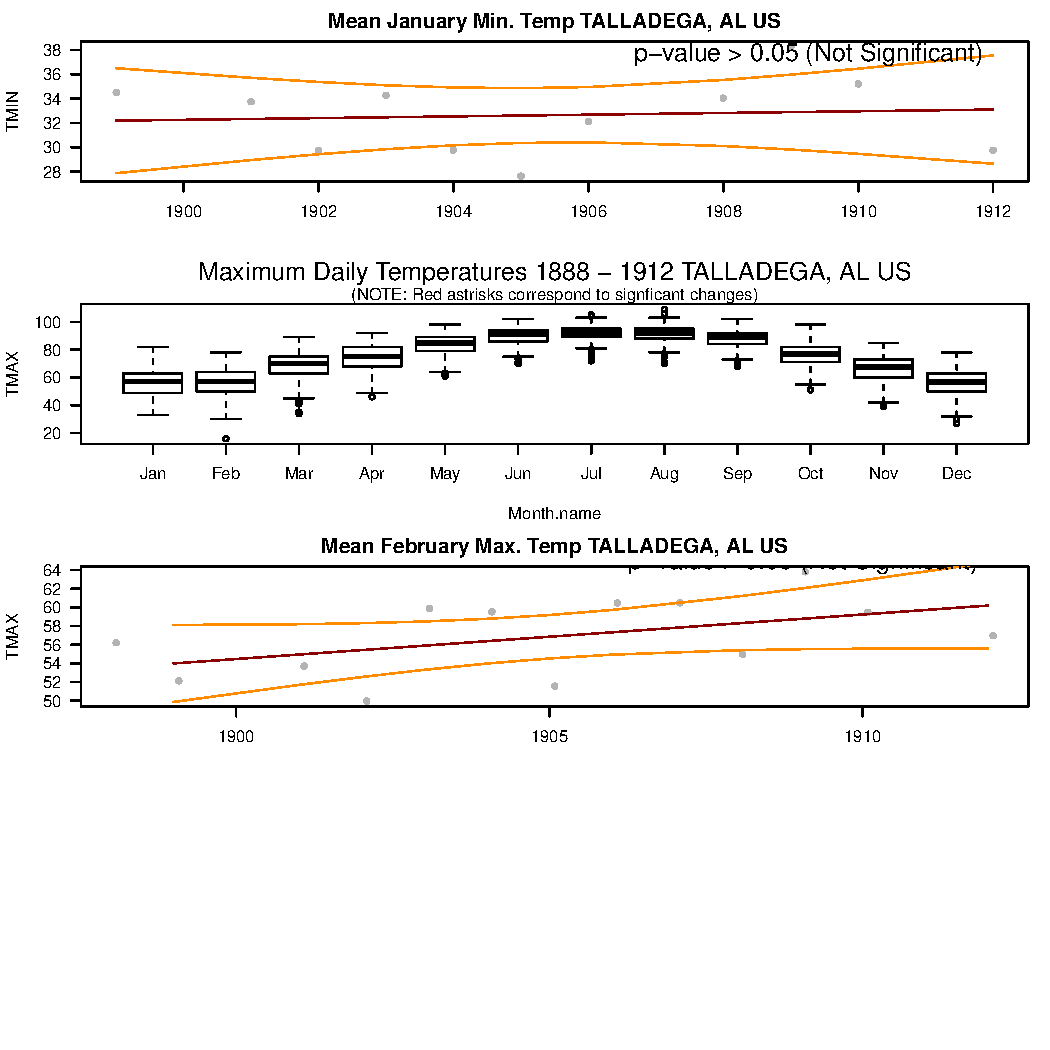
\includegraphics[width=\maxwidth]{figure/static_template-2} 

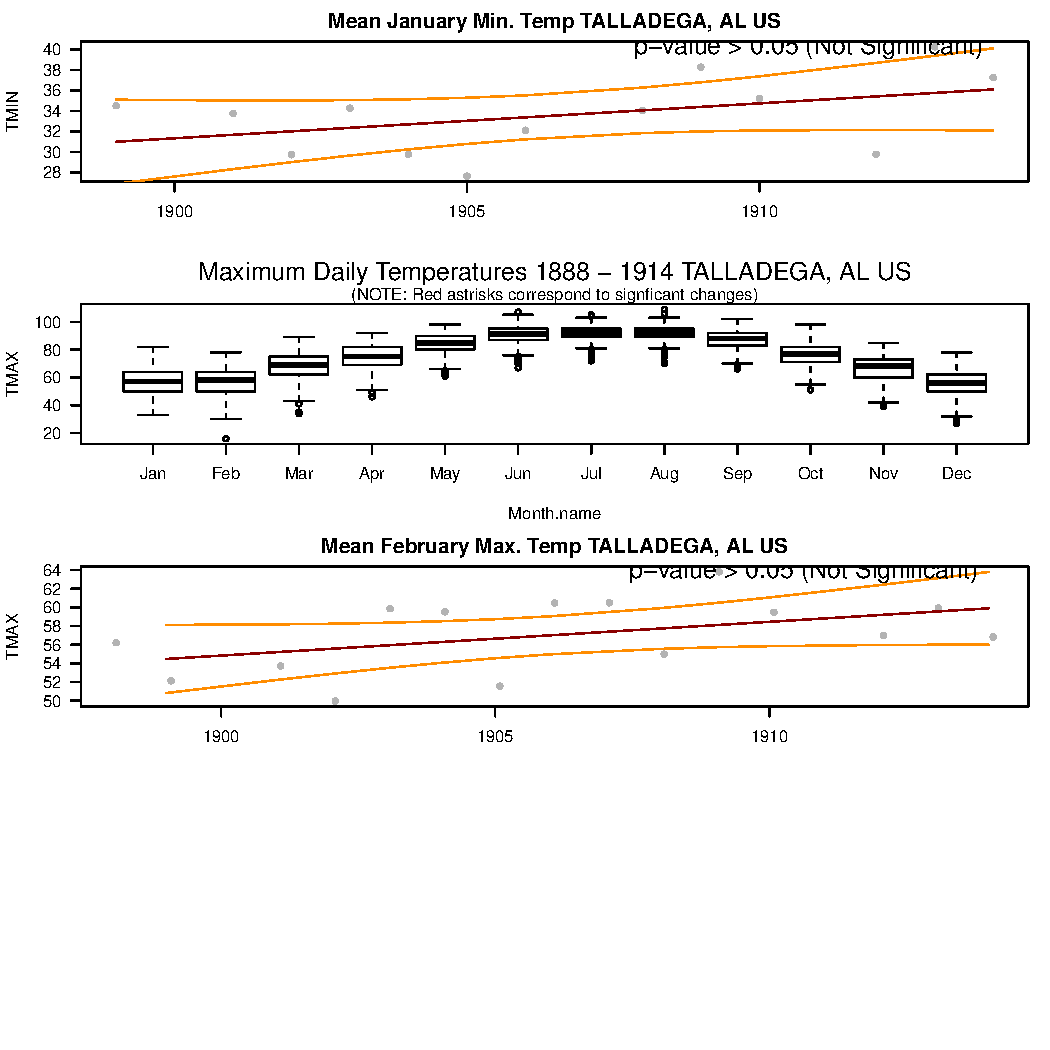
\includegraphics[width=\maxwidth]{figure/static_template-3} 

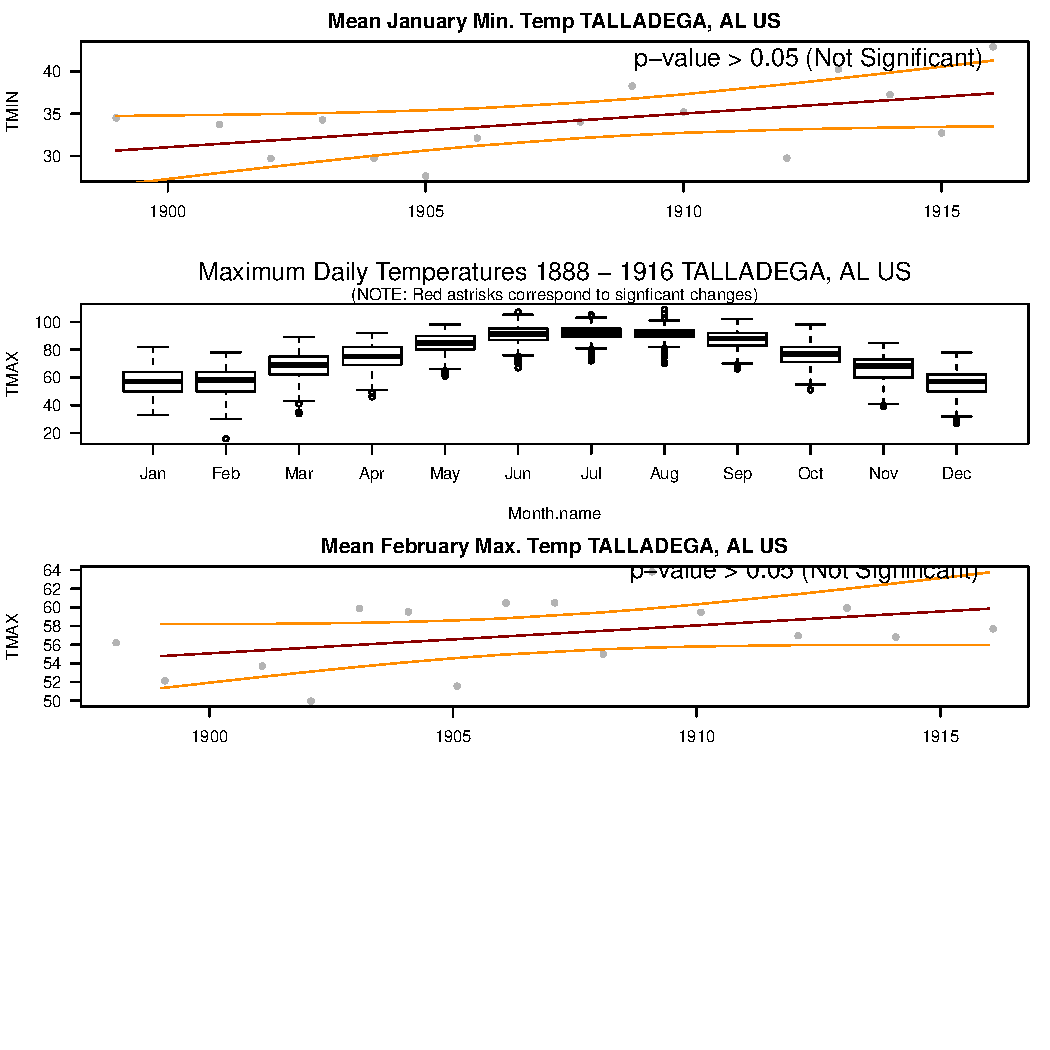
\includegraphics[width=\maxwidth]{figure/static_template-4} 

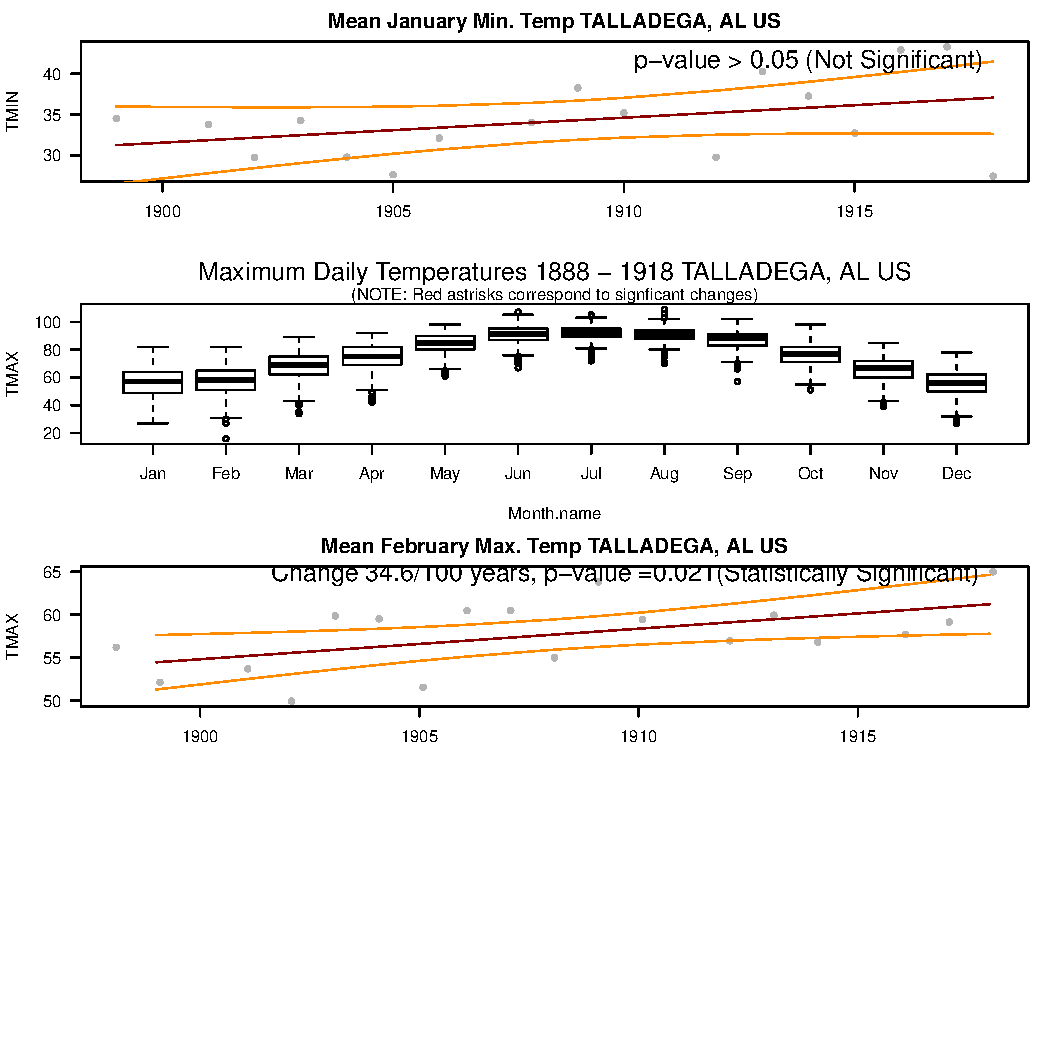
\includegraphics[width=\maxwidth]{figure/static_template-5} 

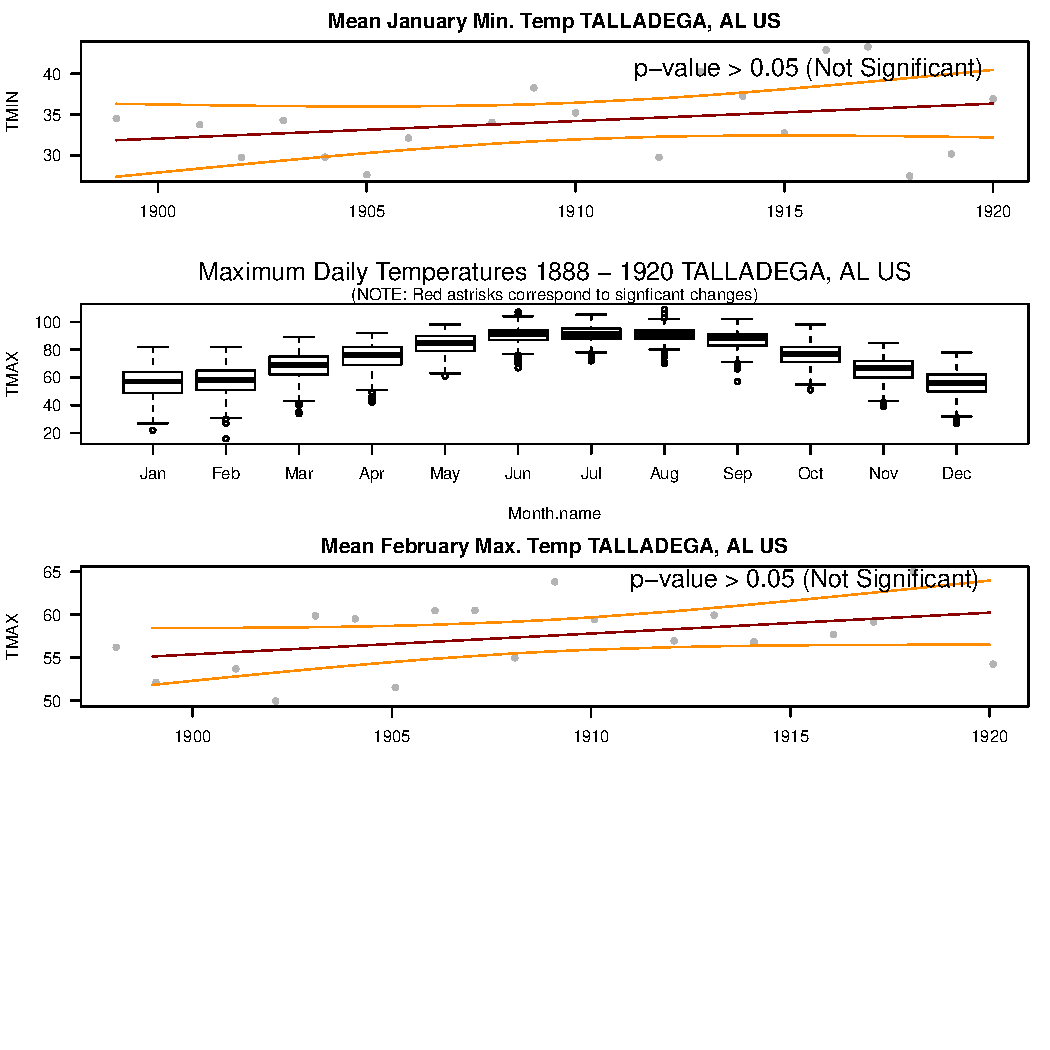
\includegraphics[width=\maxwidth]{figure/static_template-6} 

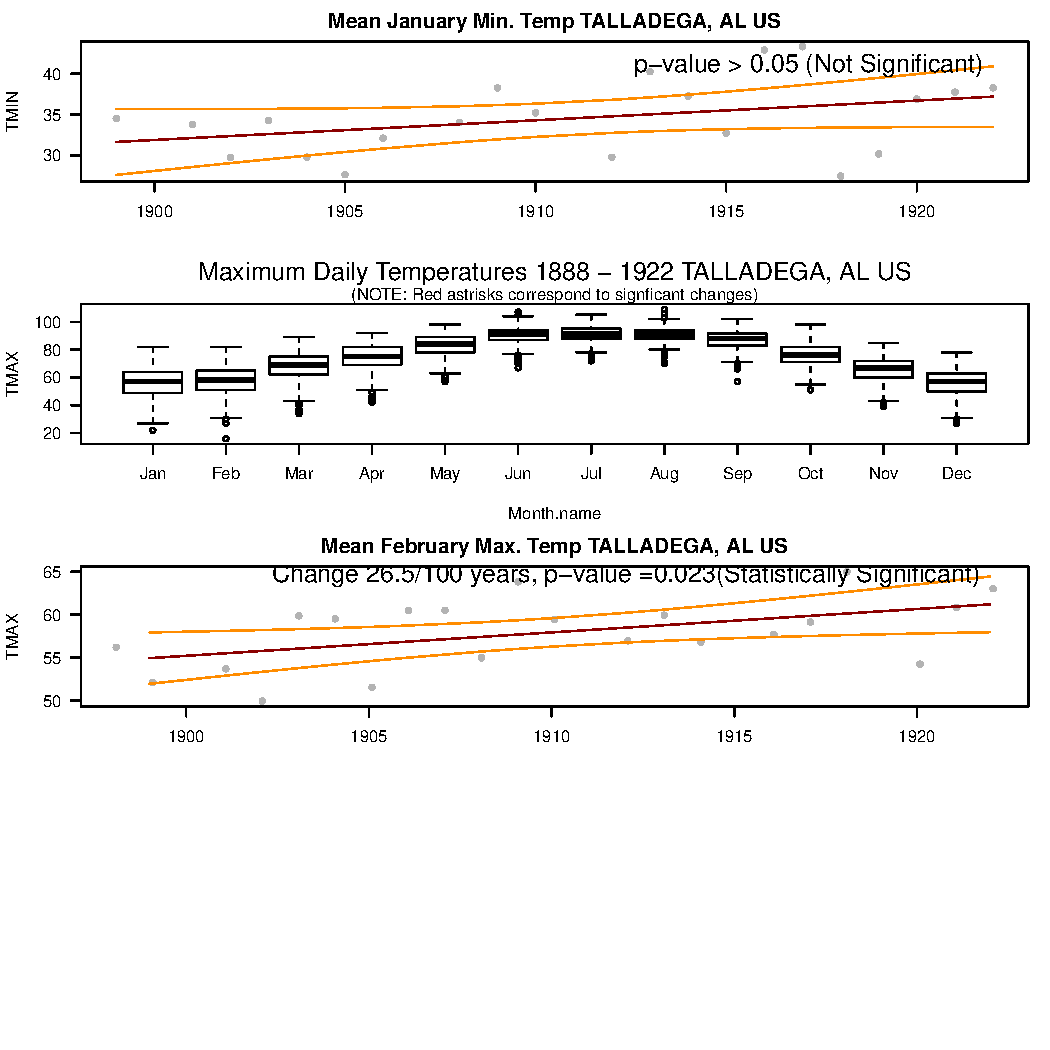
\includegraphics[width=\maxwidth]{figure/static_template-7} 

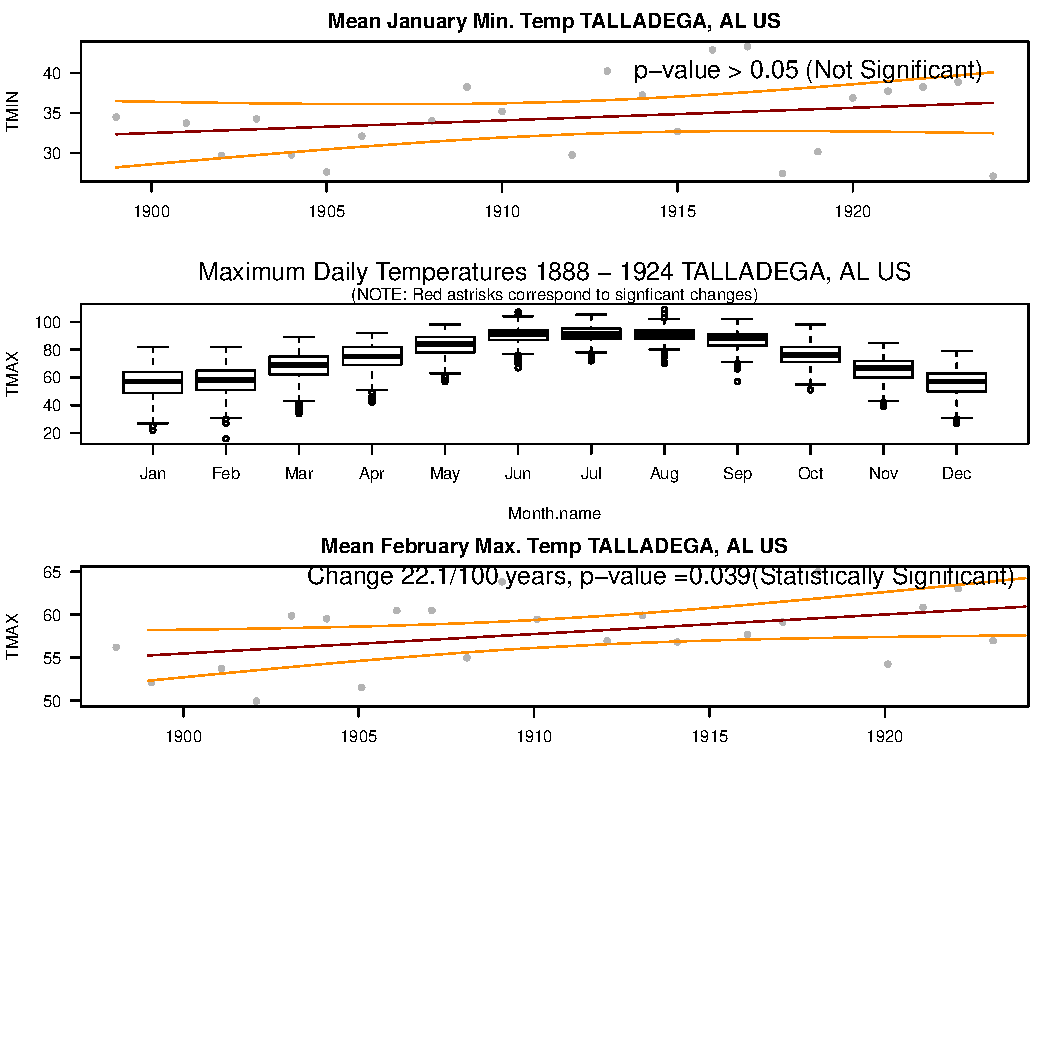
\includegraphics[width=\maxwidth]{figure/static_template-8} 

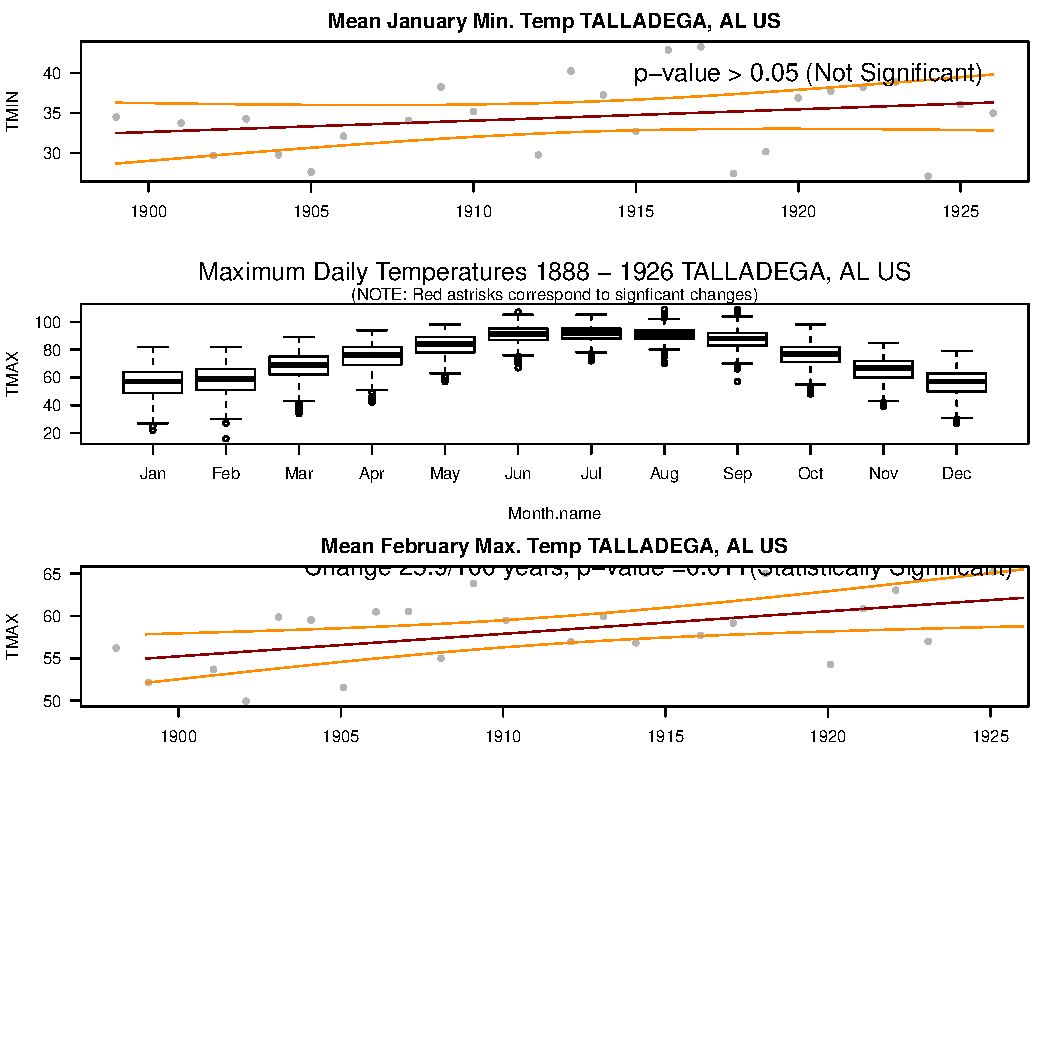
\includegraphics[width=\maxwidth]{figure/static_template-9} 

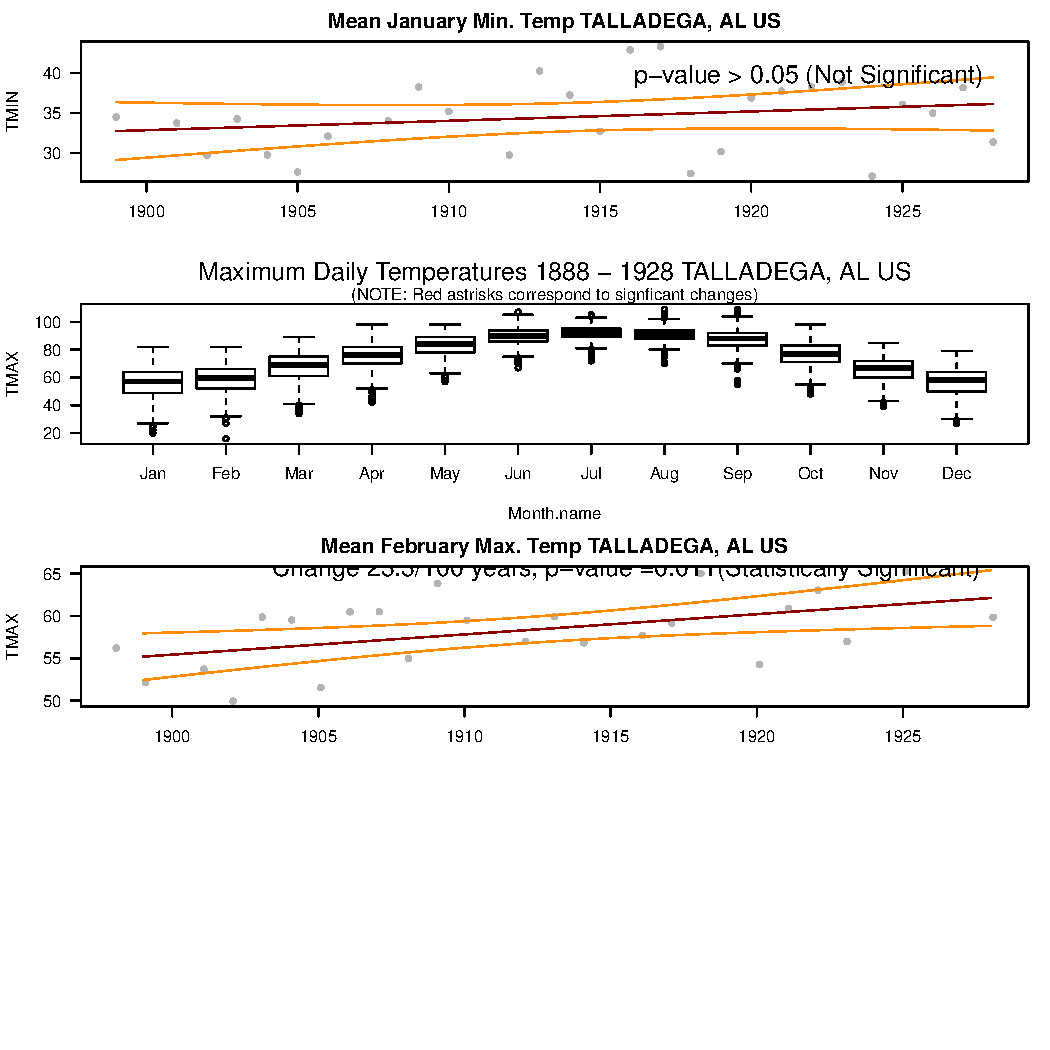
\includegraphics[width=\maxwidth]{figure/static_template-10} 

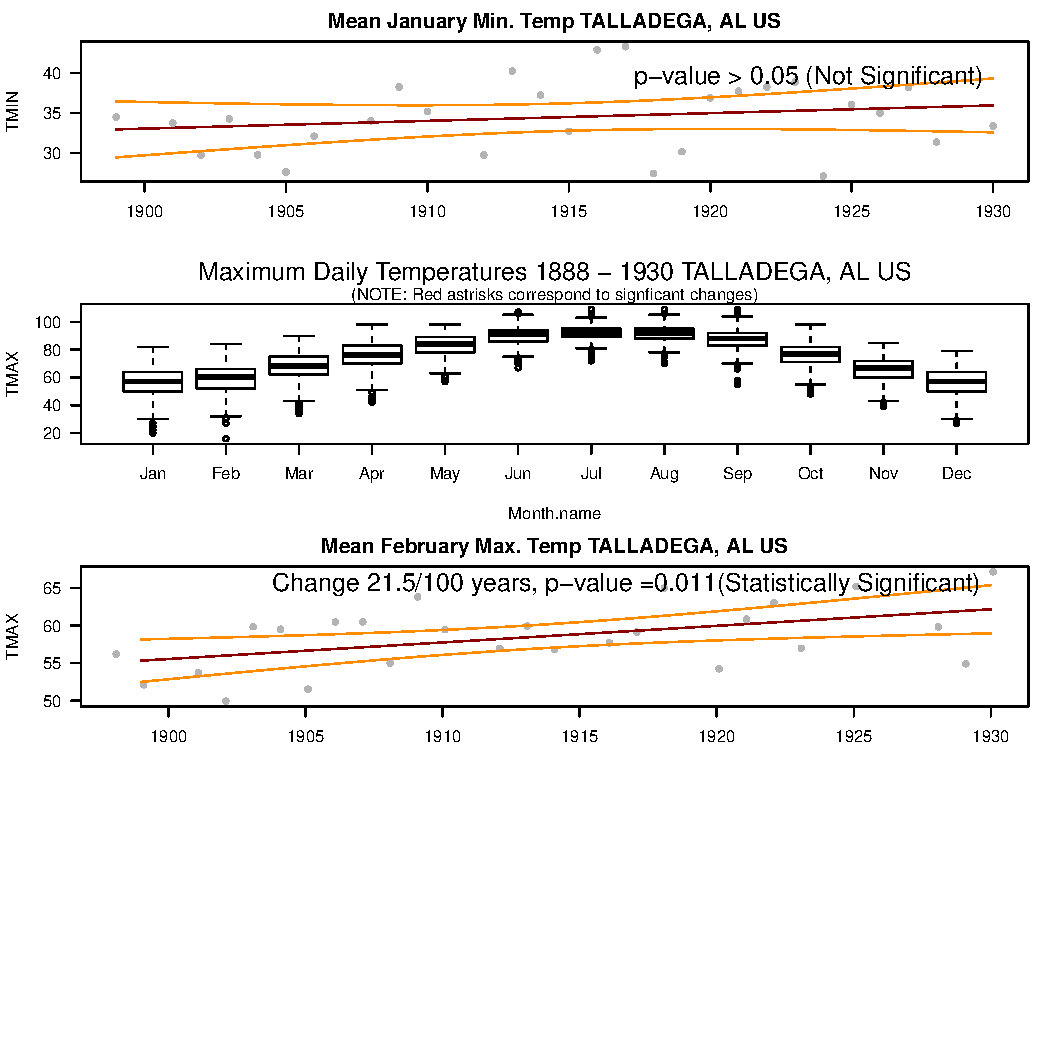
\includegraphics[width=\maxwidth]{figure/static_template-11} 

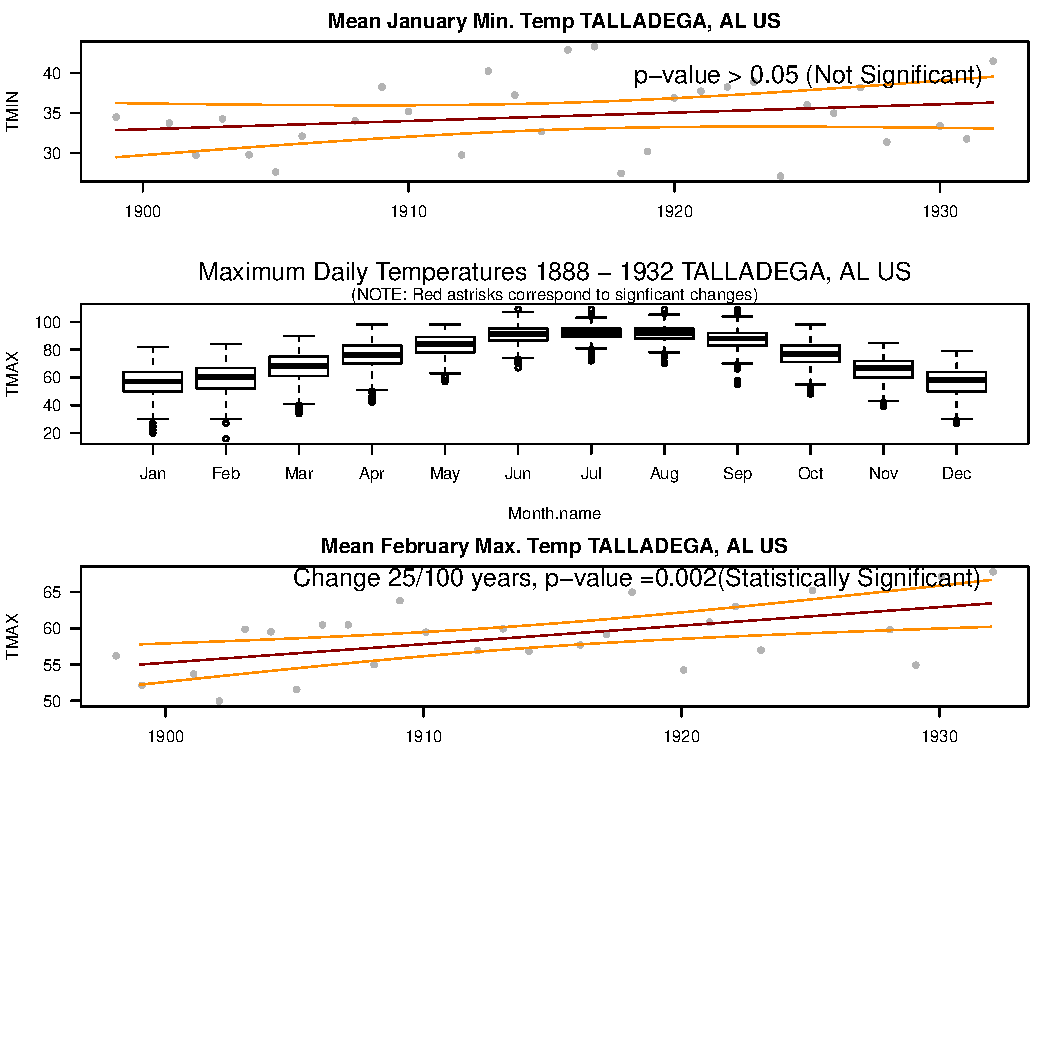
\includegraphics[width=\maxwidth]{figure/static_template-12} 

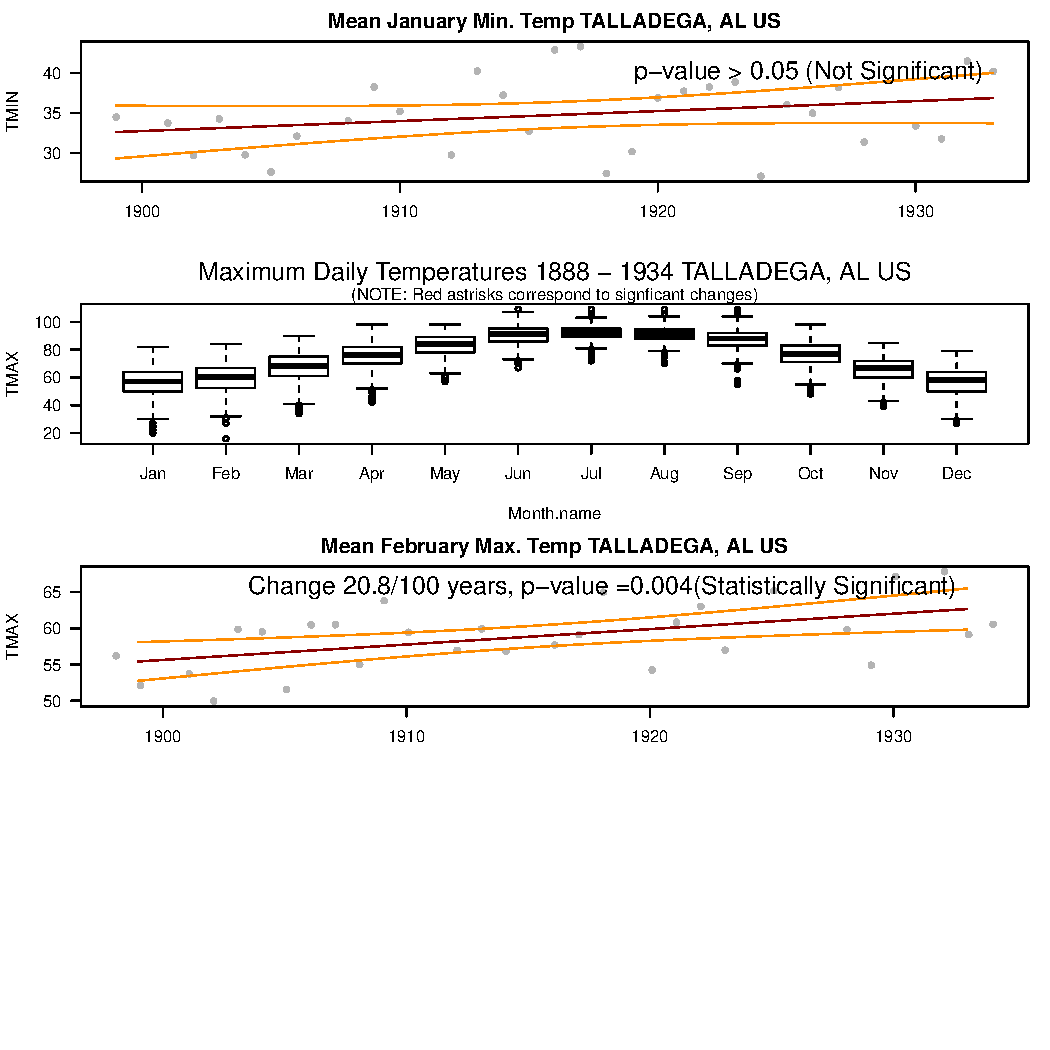
\includegraphics[width=\maxwidth]{figure/static_template-13} 

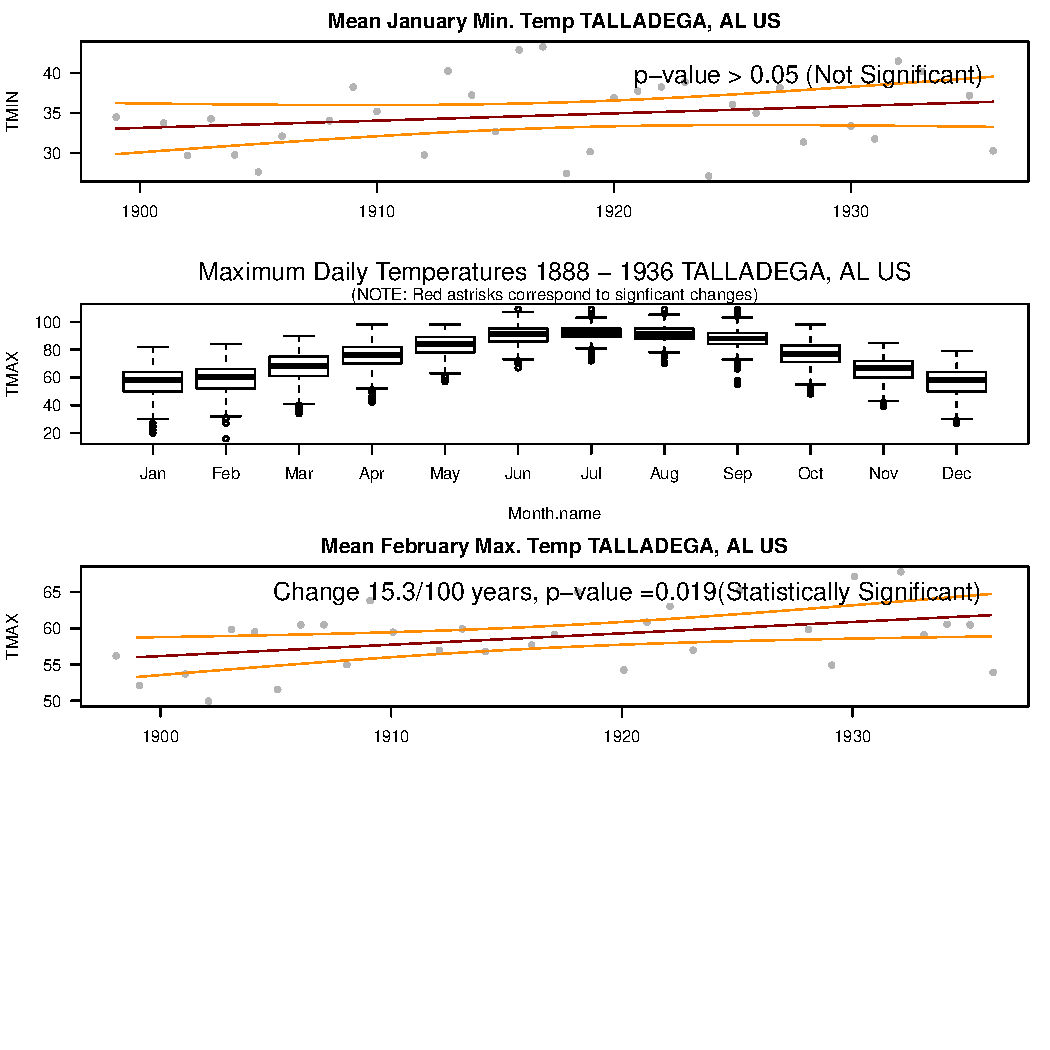
\includegraphics[width=\maxwidth]{figure/static_template-14} 

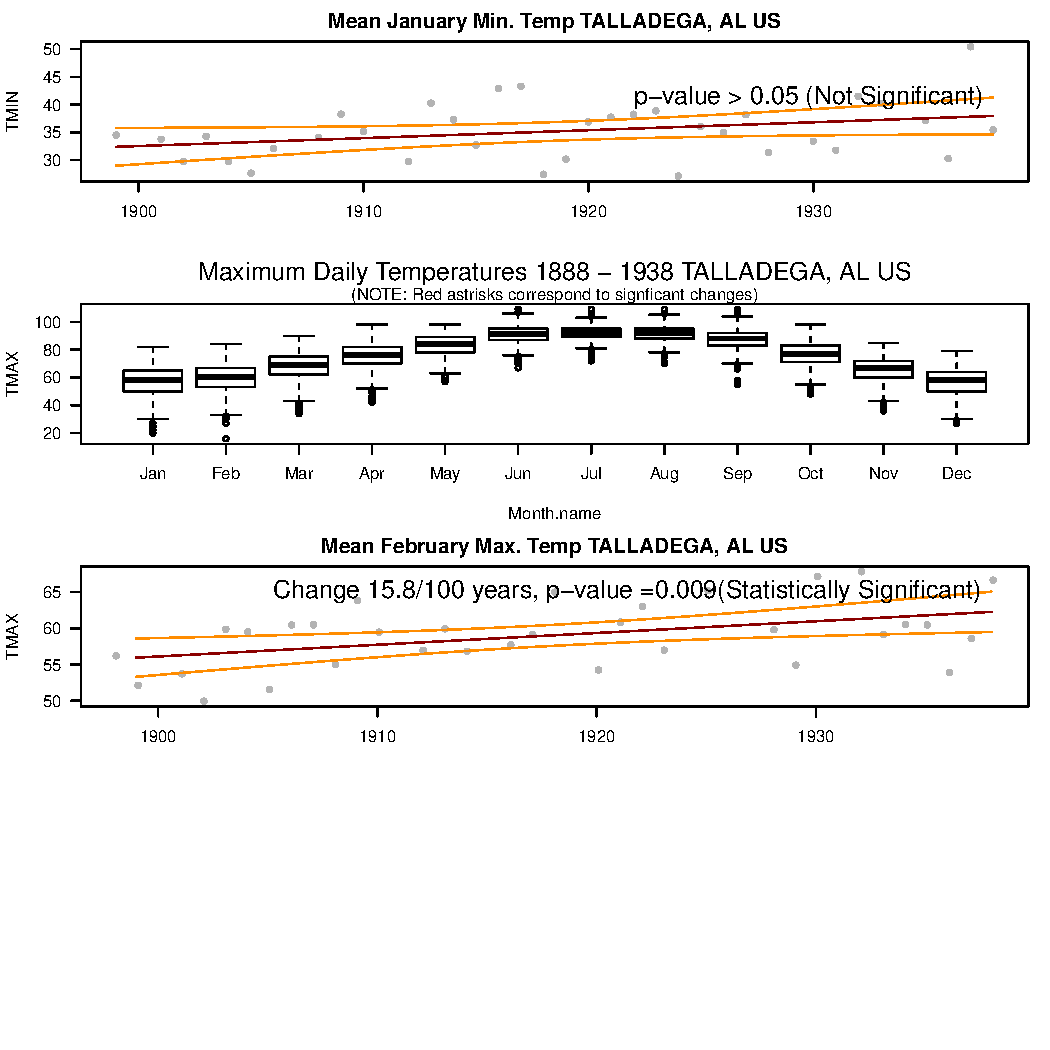
\includegraphics[width=\maxwidth]{figure/static_template-15} 

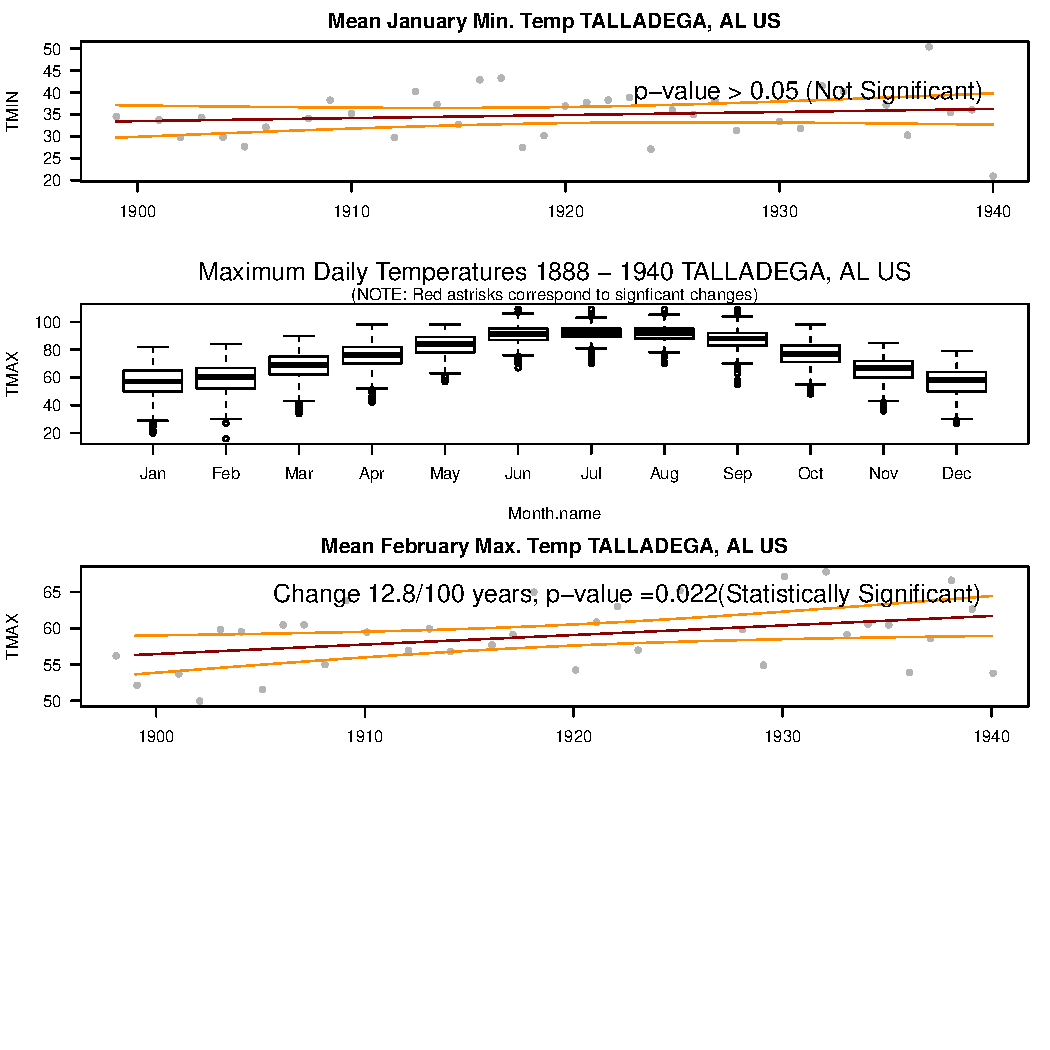
\includegraphics[width=\maxwidth]{figure/static_template-16} 

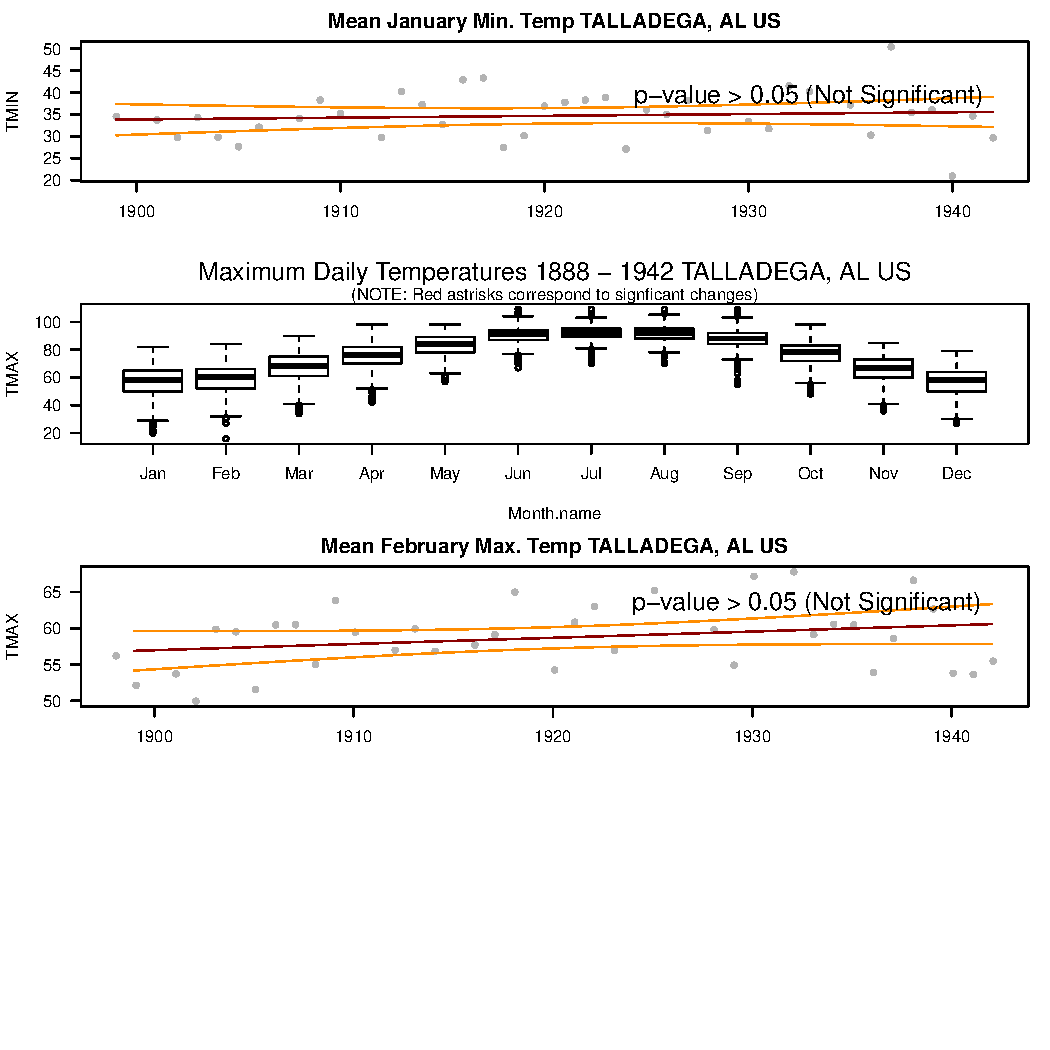
\includegraphics[width=\maxwidth]{figure/static_template-17} 

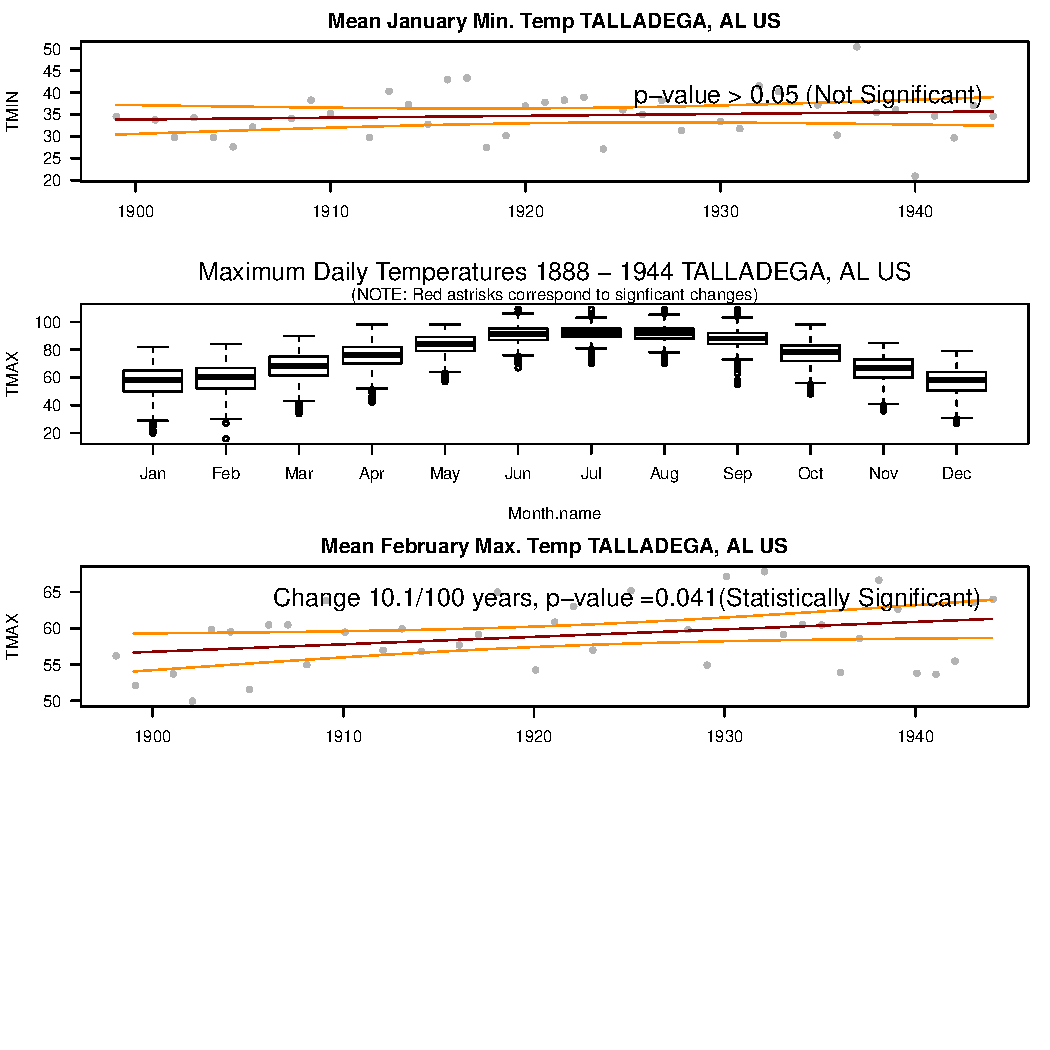
\includegraphics[width=\maxwidth]{figure/static_template-18} 

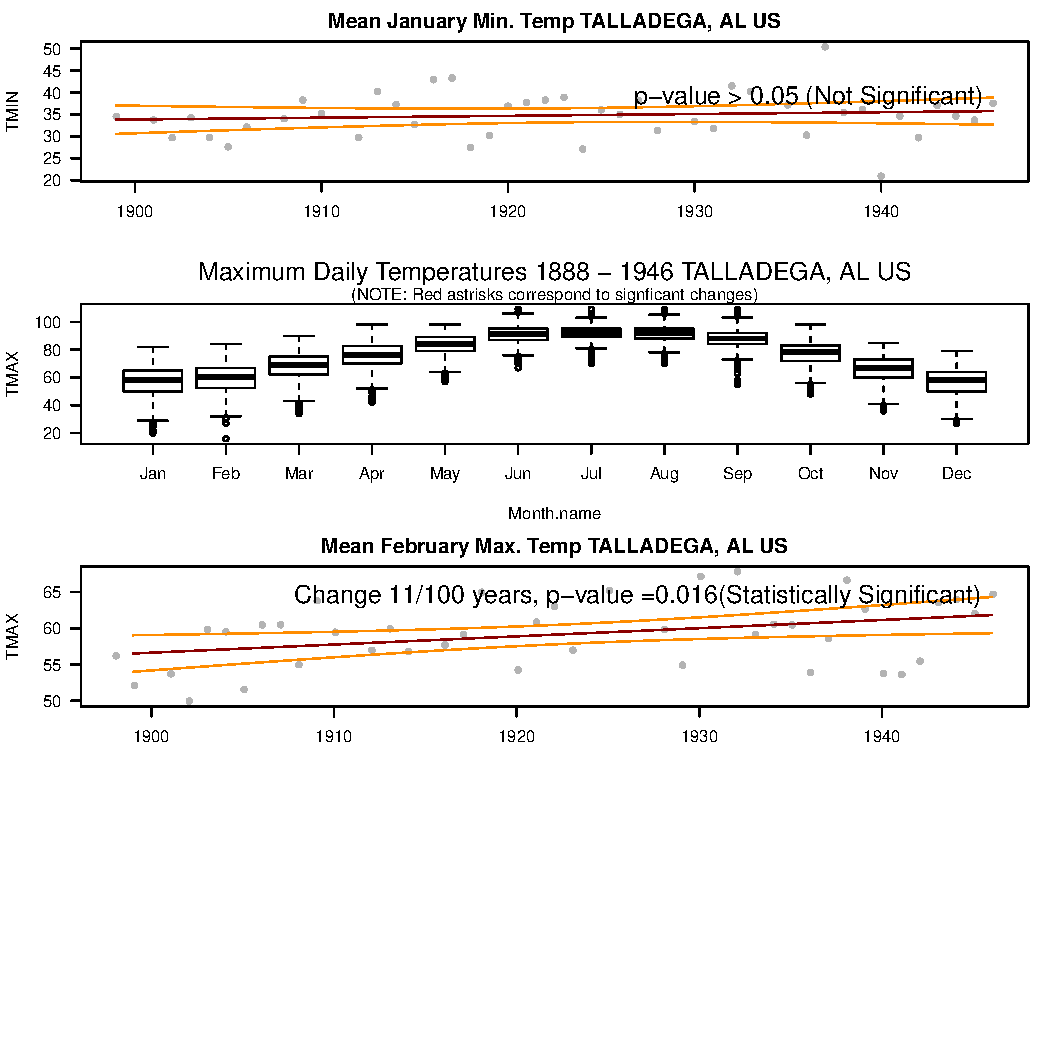
\includegraphics[width=\maxwidth]{figure/static_template-19} 

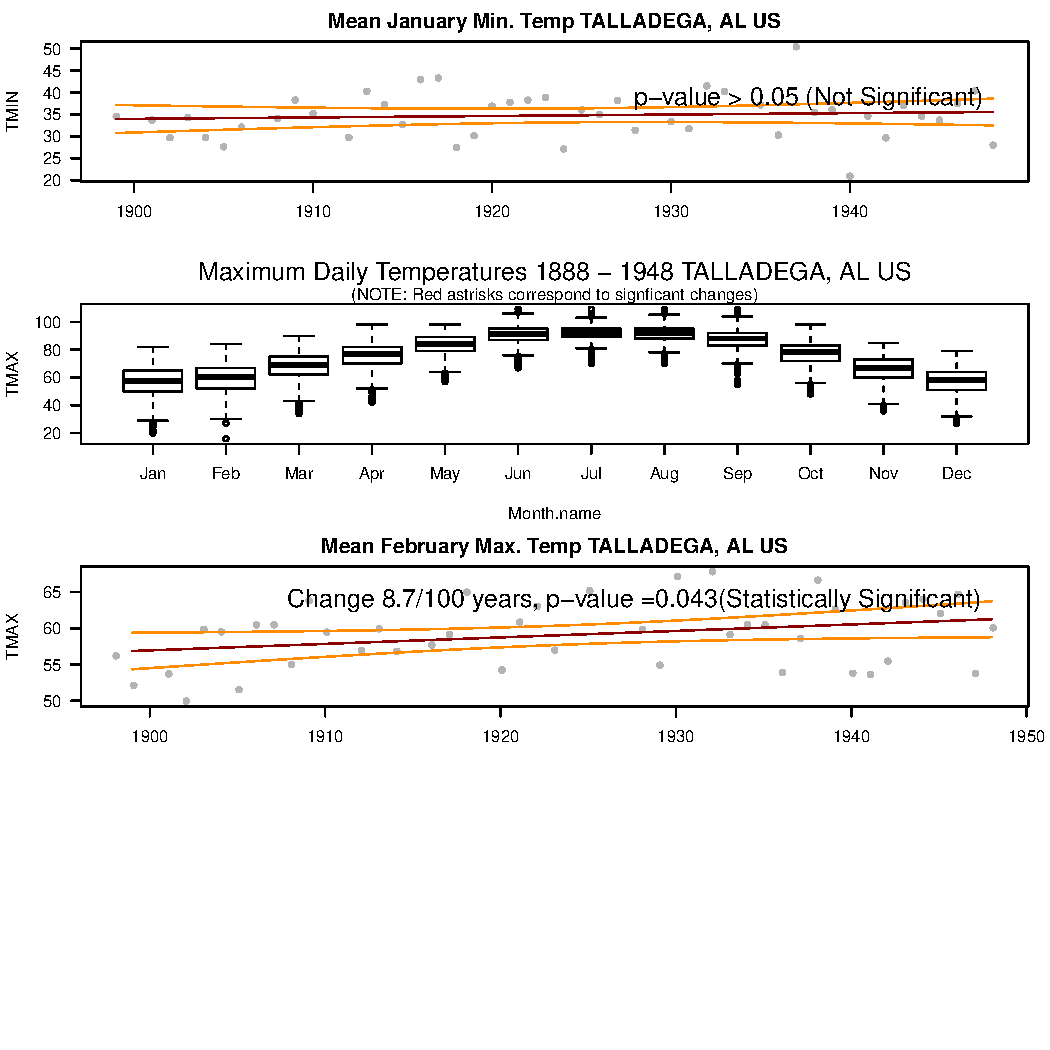
\includegraphics[width=\maxwidth]{figure/static_template-20} 

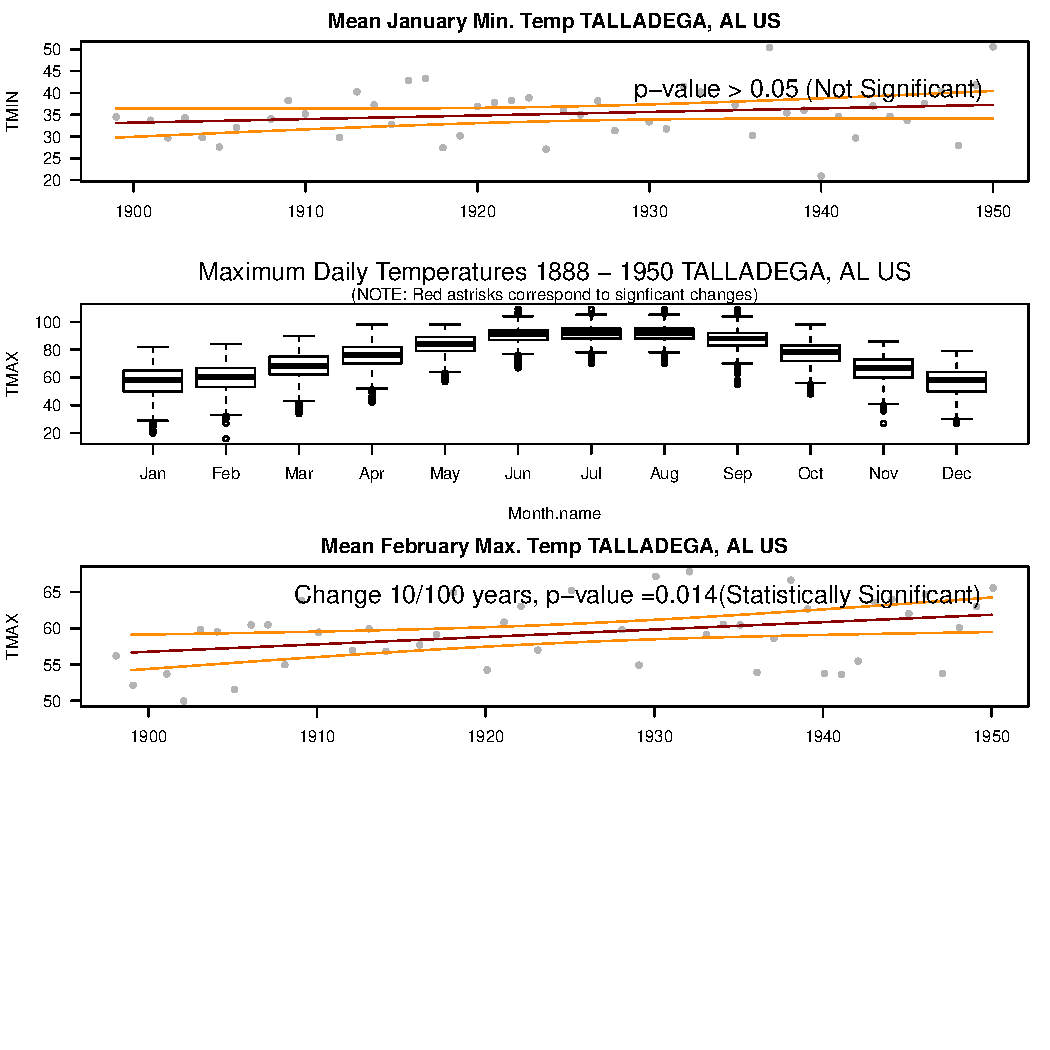
\includegraphics[width=\maxwidth]{figure/static_template-21} 

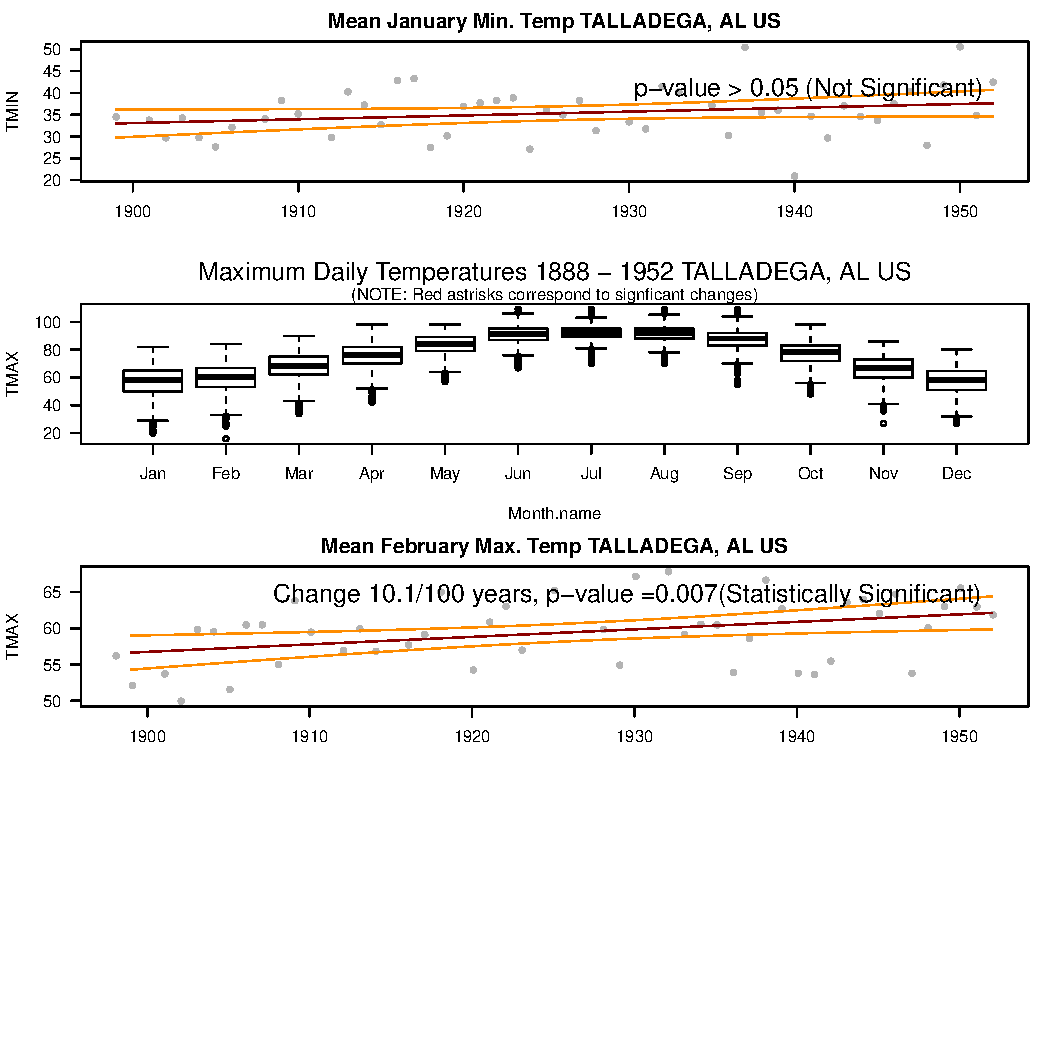
\includegraphics[width=\maxwidth]{figure/static_template-22} 

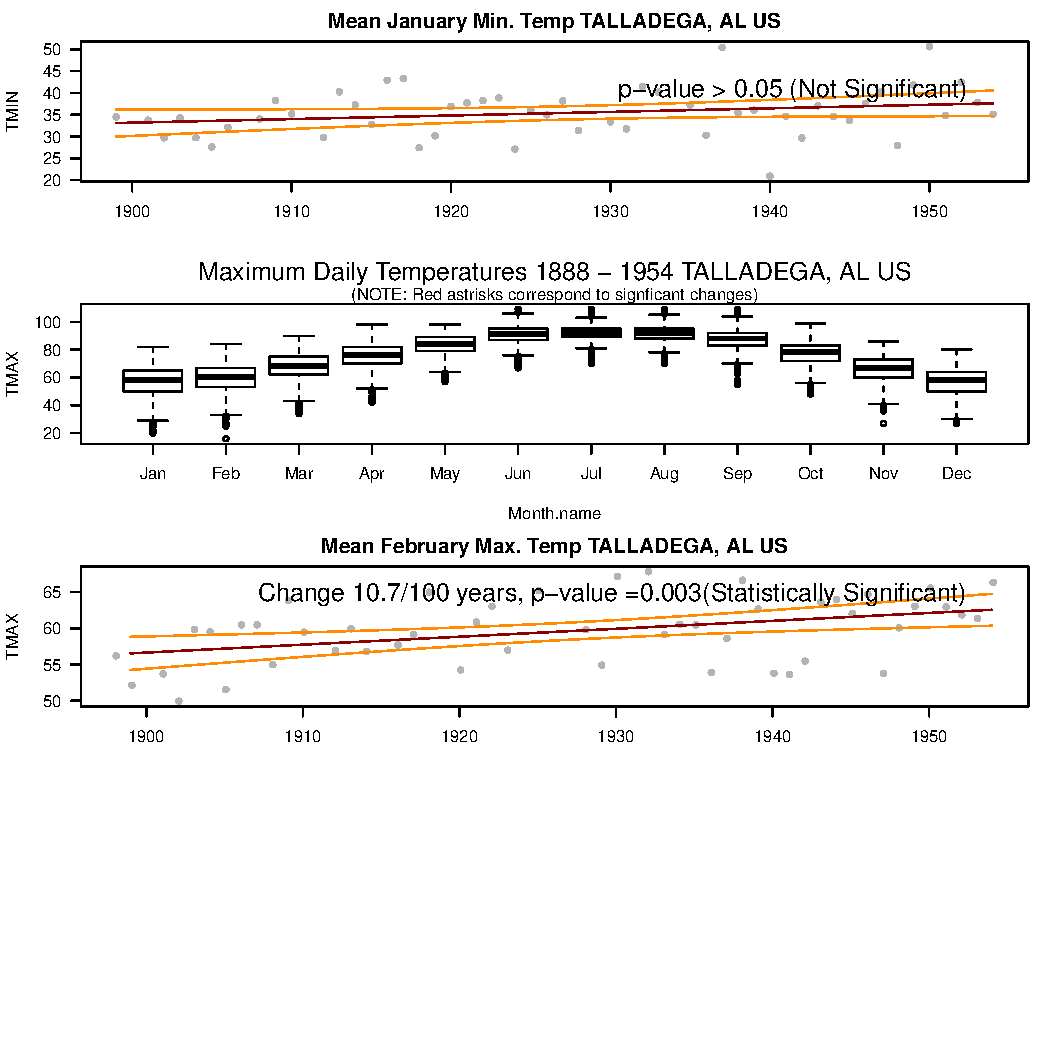
\includegraphics[width=\maxwidth]{figure/static_template-23} 

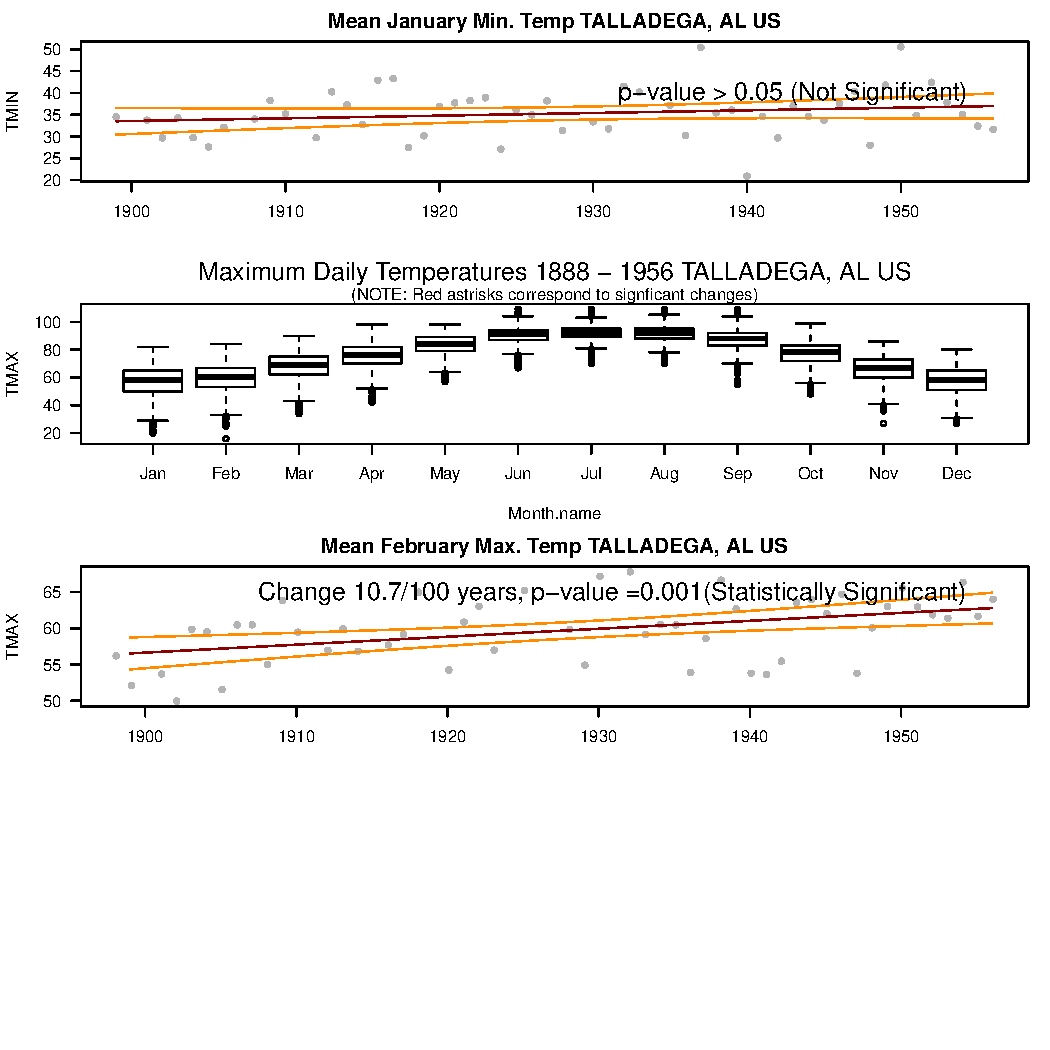
\includegraphics[width=\maxwidth]{figure/static_template-24} 

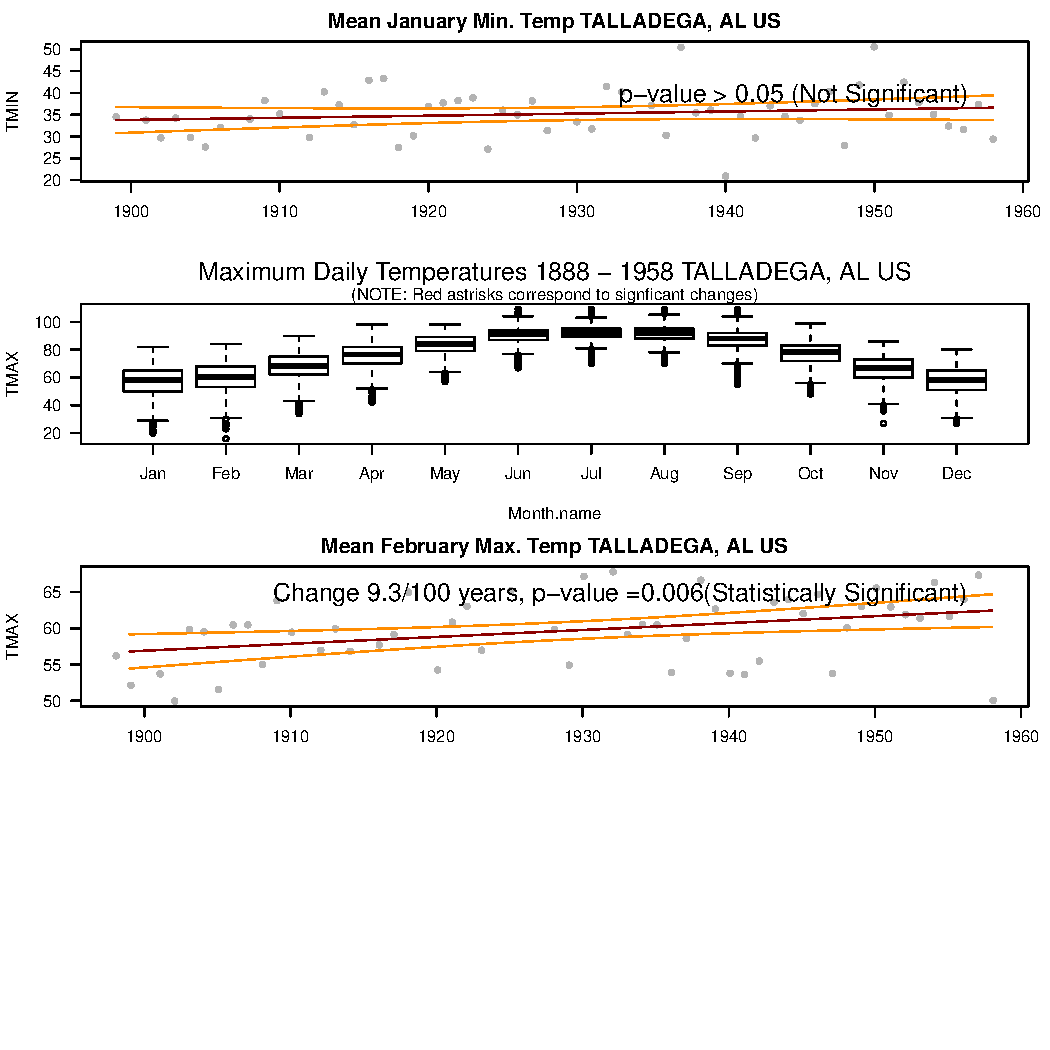
\includegraphics[width=\maxwidth]{figure/static_template-25} 

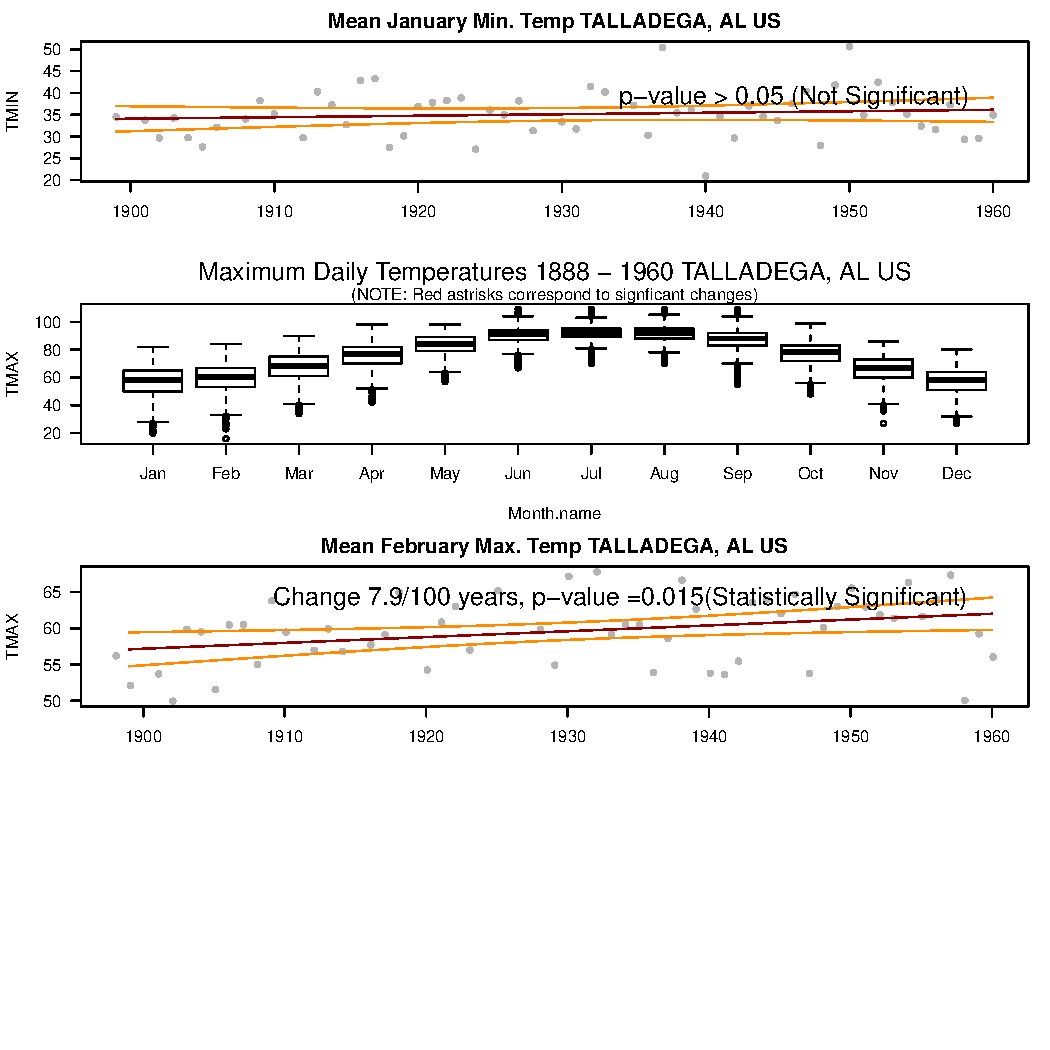
\includegraphics[width=\maxwidth]{figure/static_template-26} 

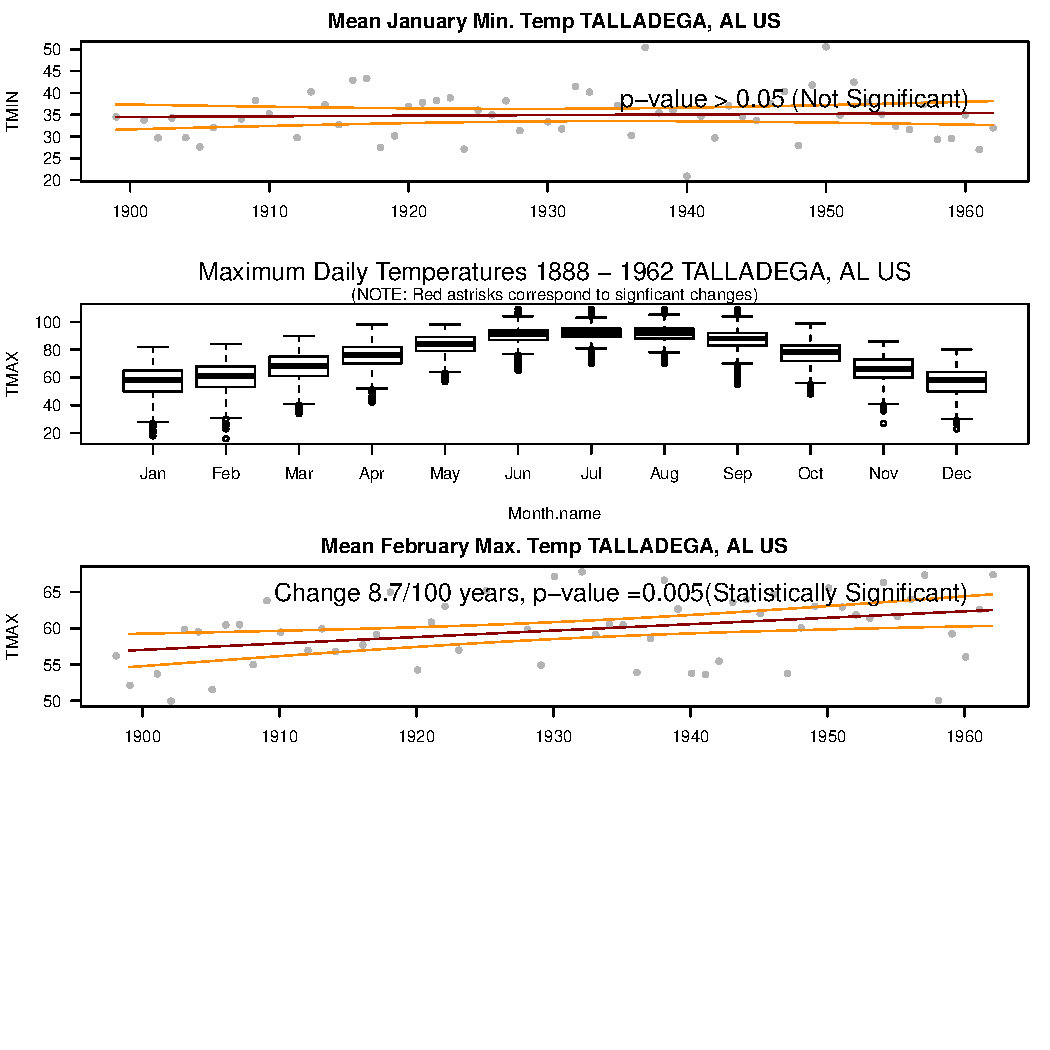
\includegraphics[width=\maxwidth]{figure/static_template-27} 

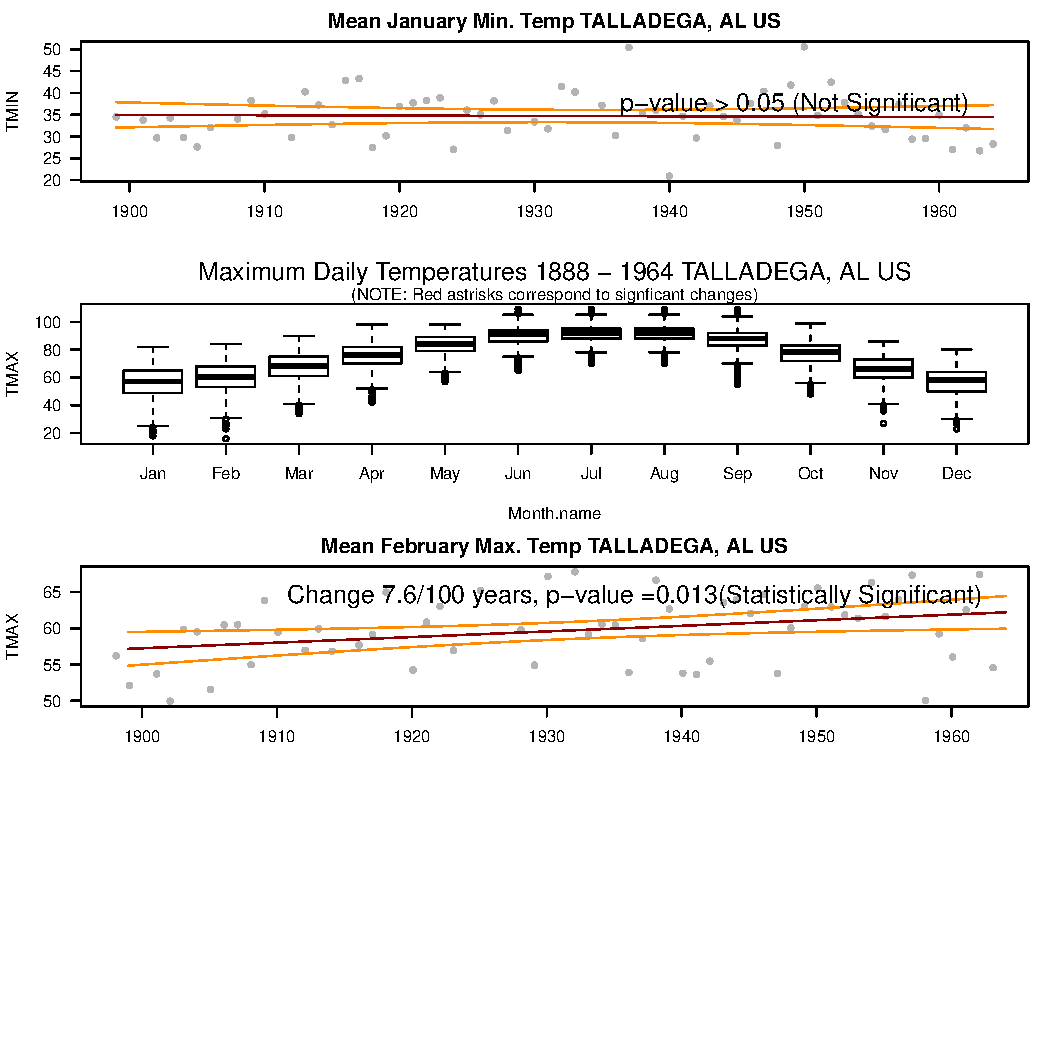
\includegraphics[width=\maxwidth]{figure/static_template-28} 

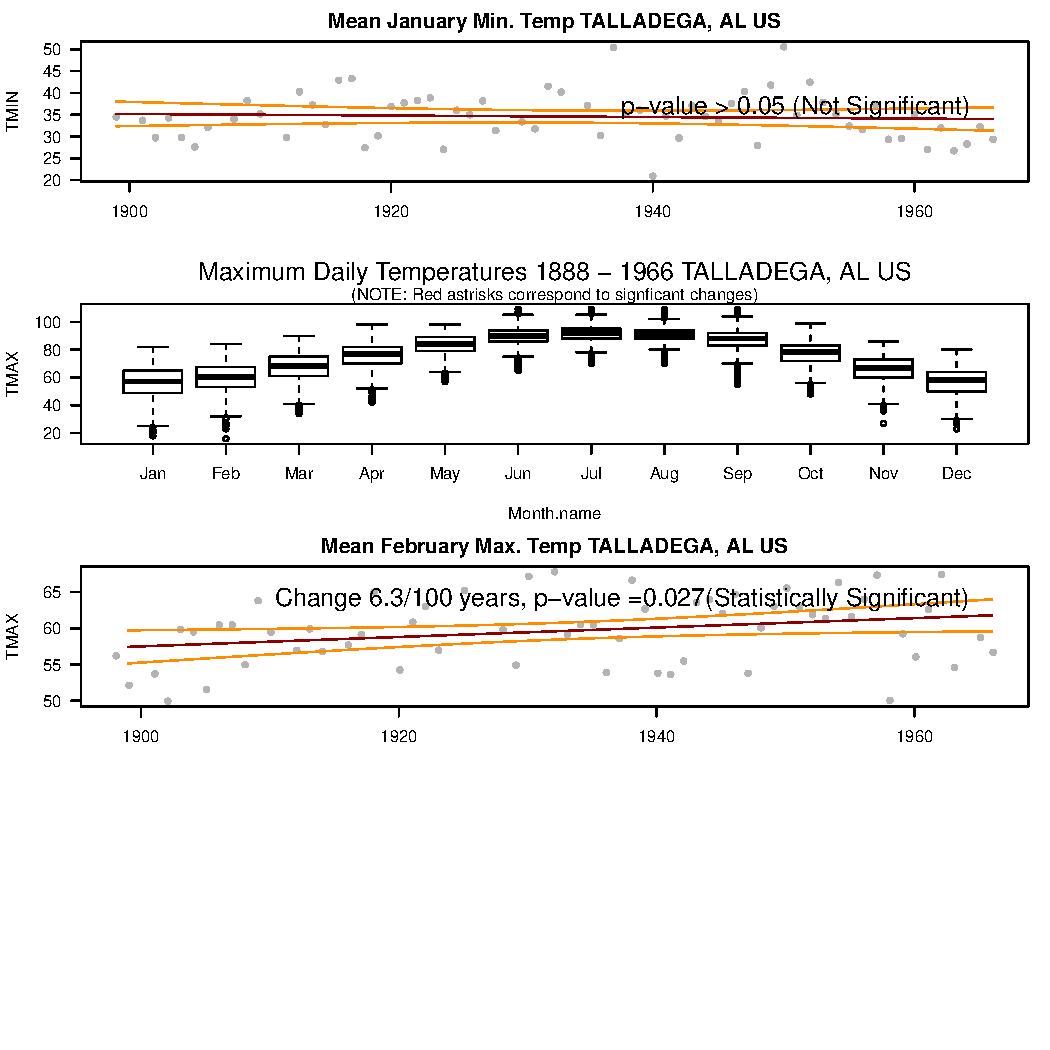
\includegraphics[width=\maxwidth]{figure/static_template-29} 

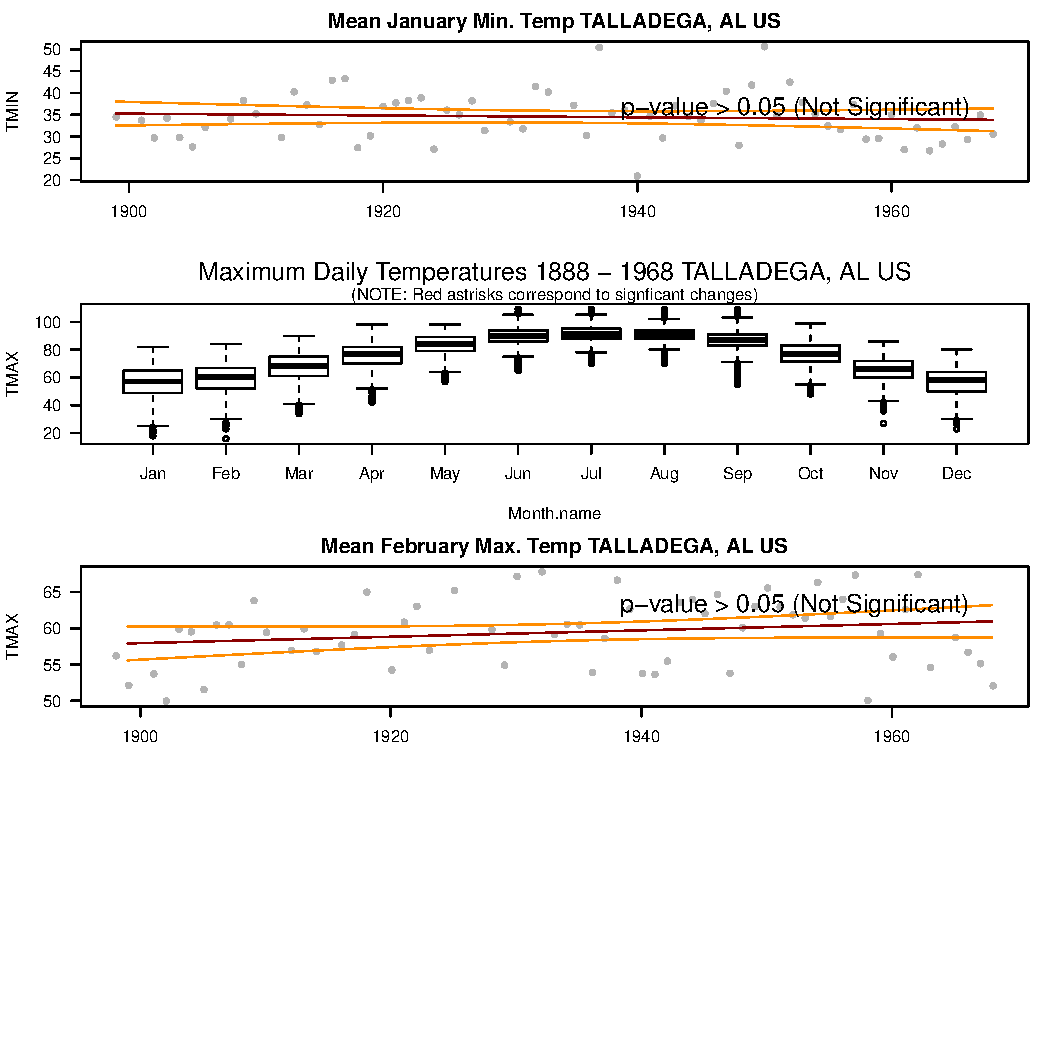
\includegraphics[width=\maxwidth]{figure/static_template-30} 

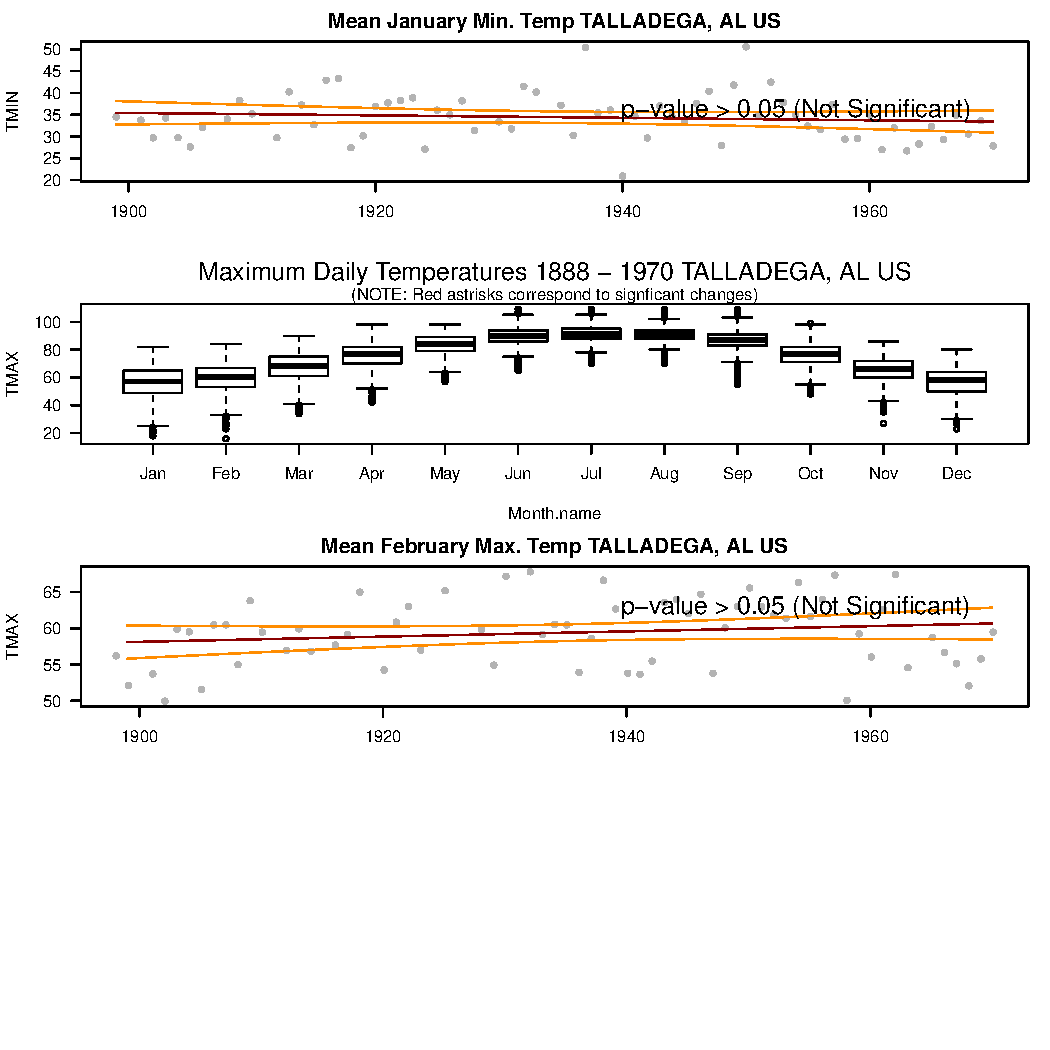
\includegraphics[width=\maxwidth]{figure/static_template-31} 

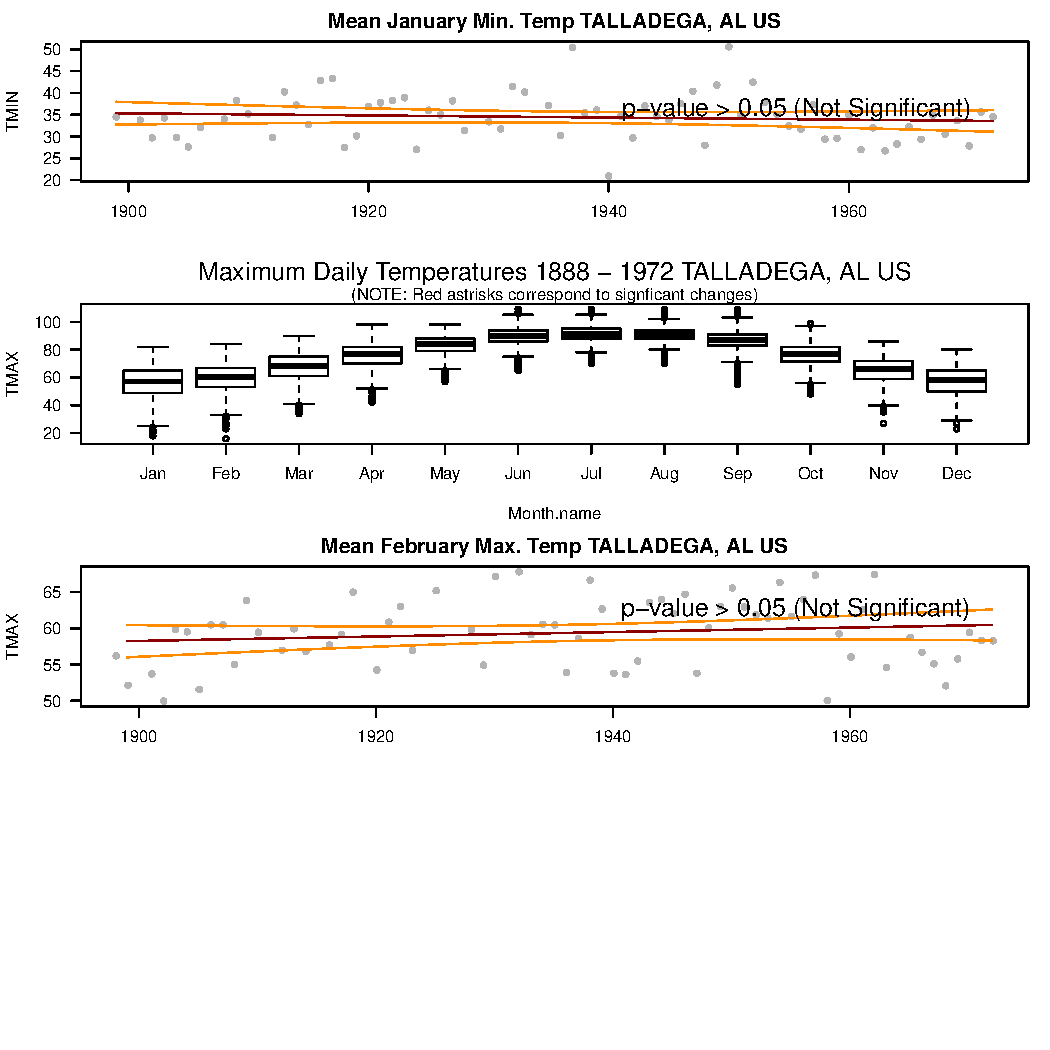
\includegraphics[width=\maxwidth]{figure/static_template-32} 

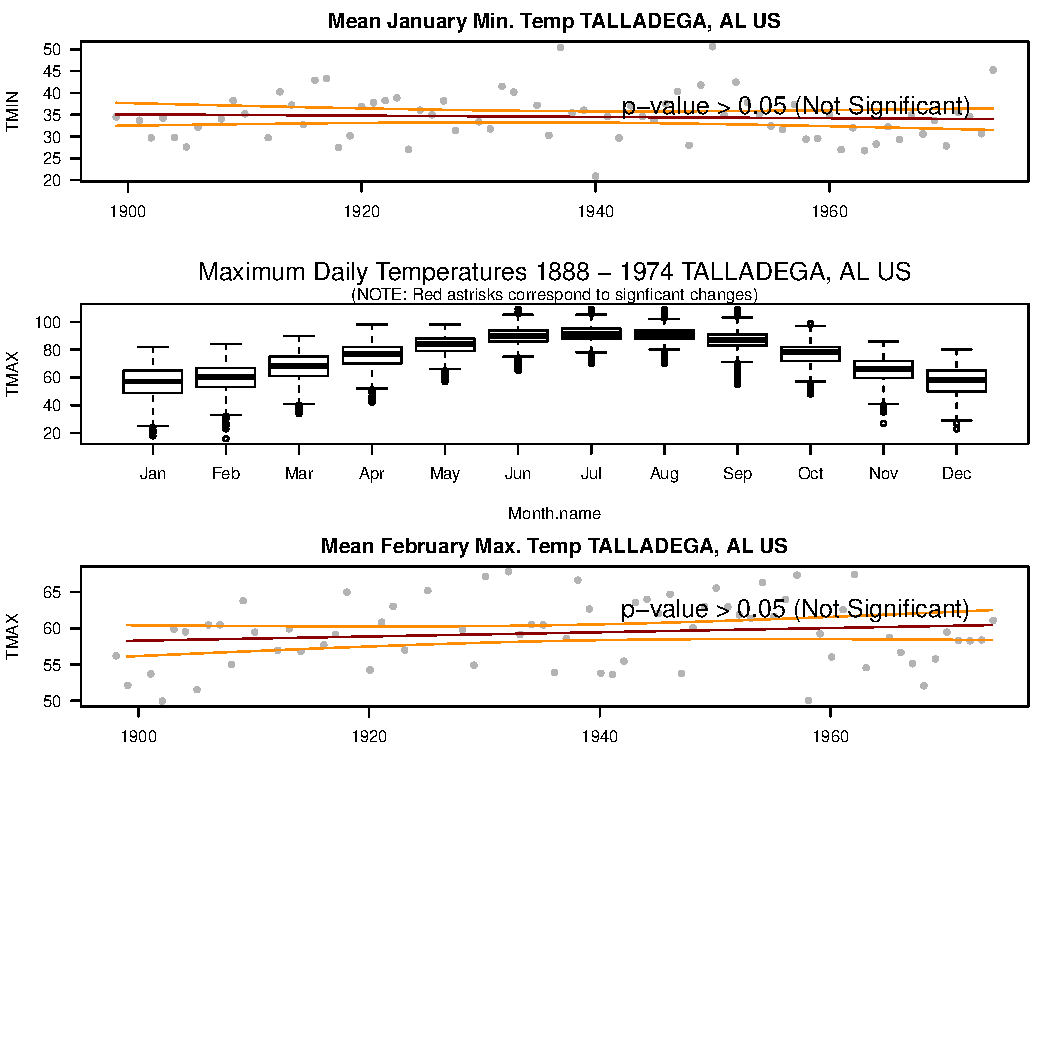
\includegraphics[width=\maxwidth]{figure/static_template-33} 

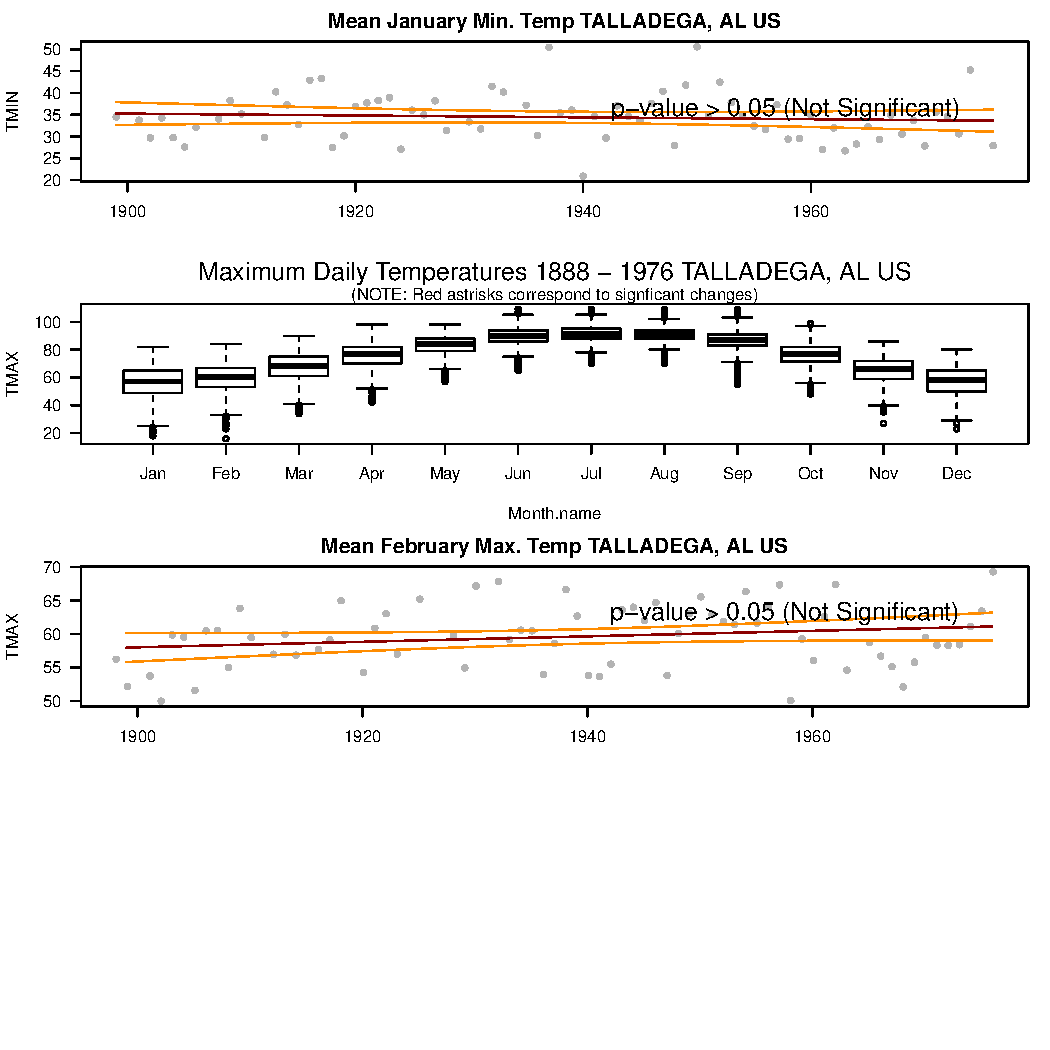
\includegraphics[width=\maxwidth]{figure/static_template-34} 

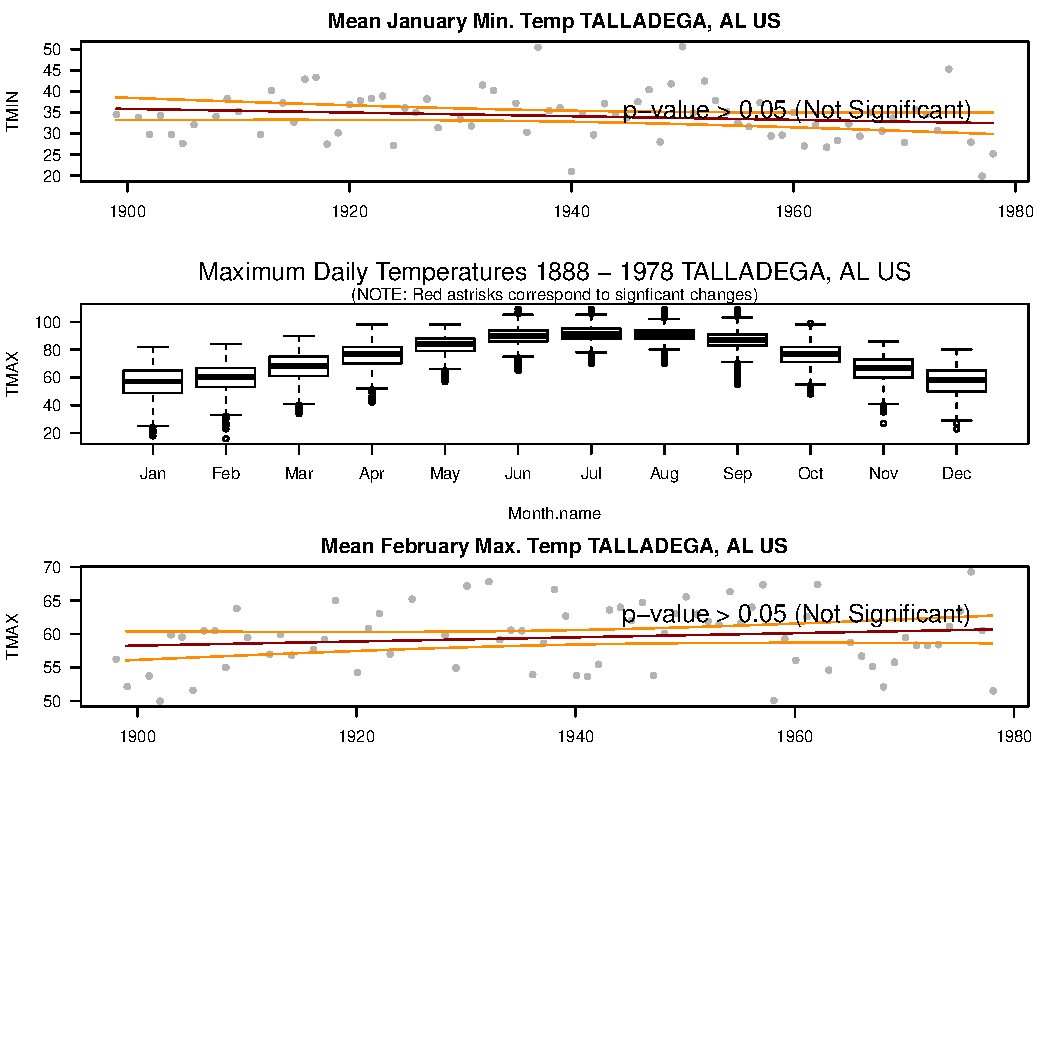
\includegraphics[width=\maxwidth]{figure/static_template-35} 

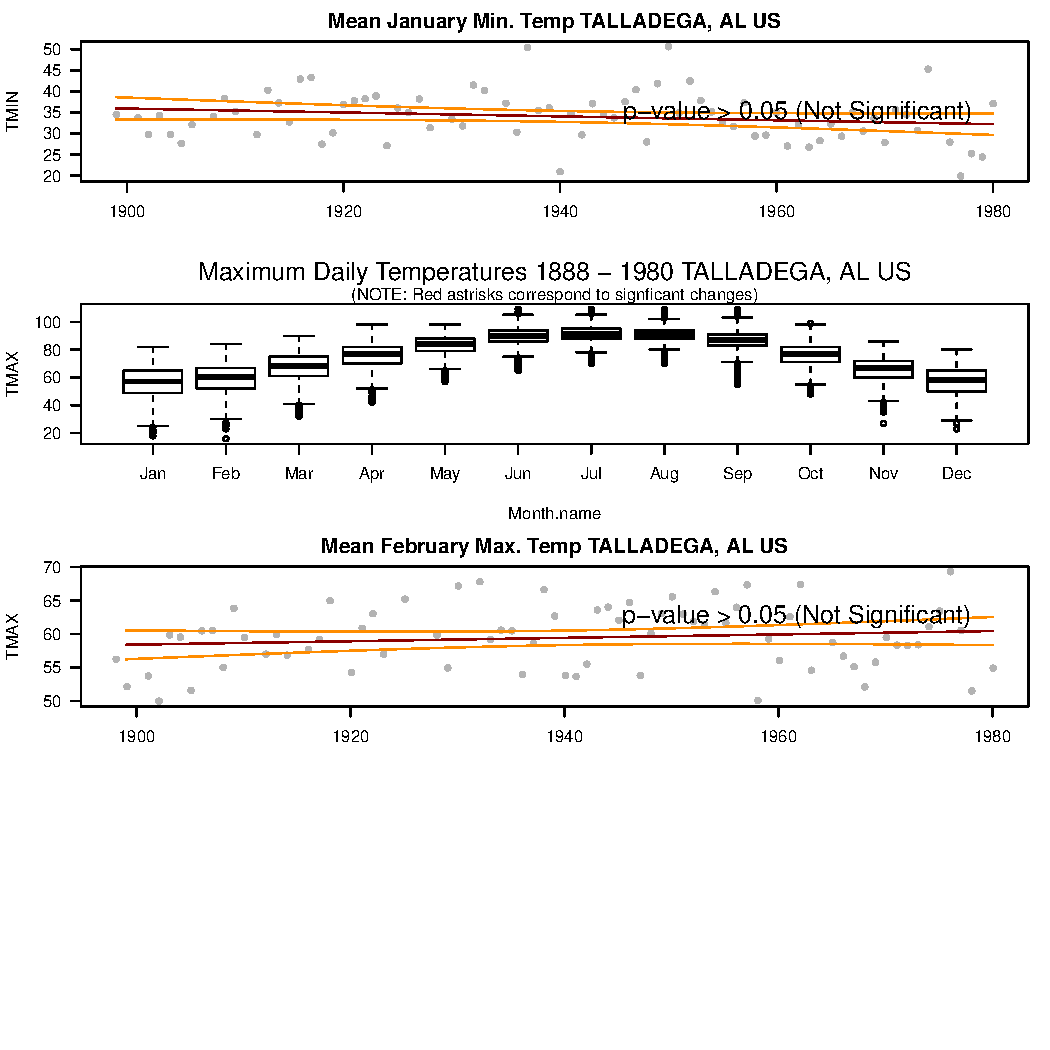
\includegraphics[width=\maxwidth]{figure/static_template-36} 

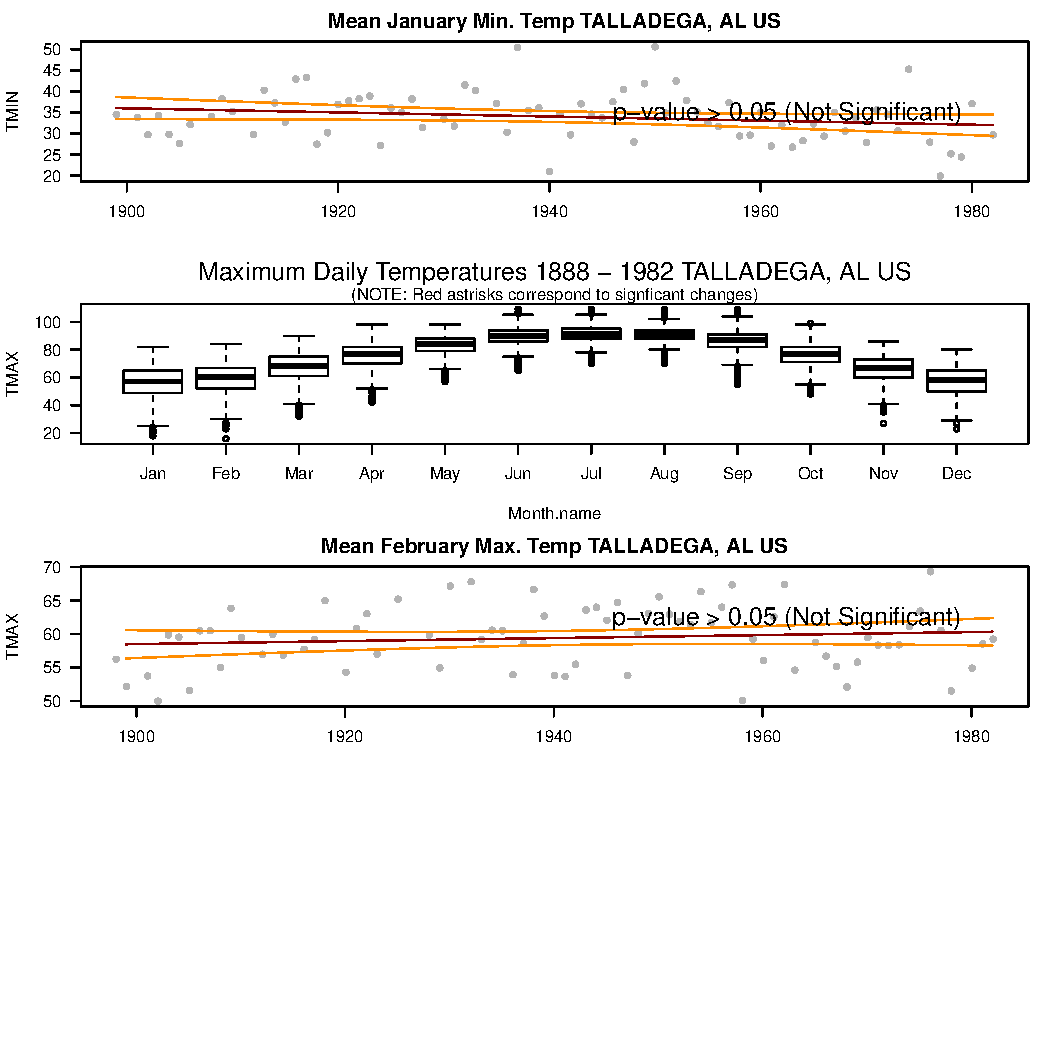
\includegraphics[width=\maxwidth]{figure/static_template-37} 

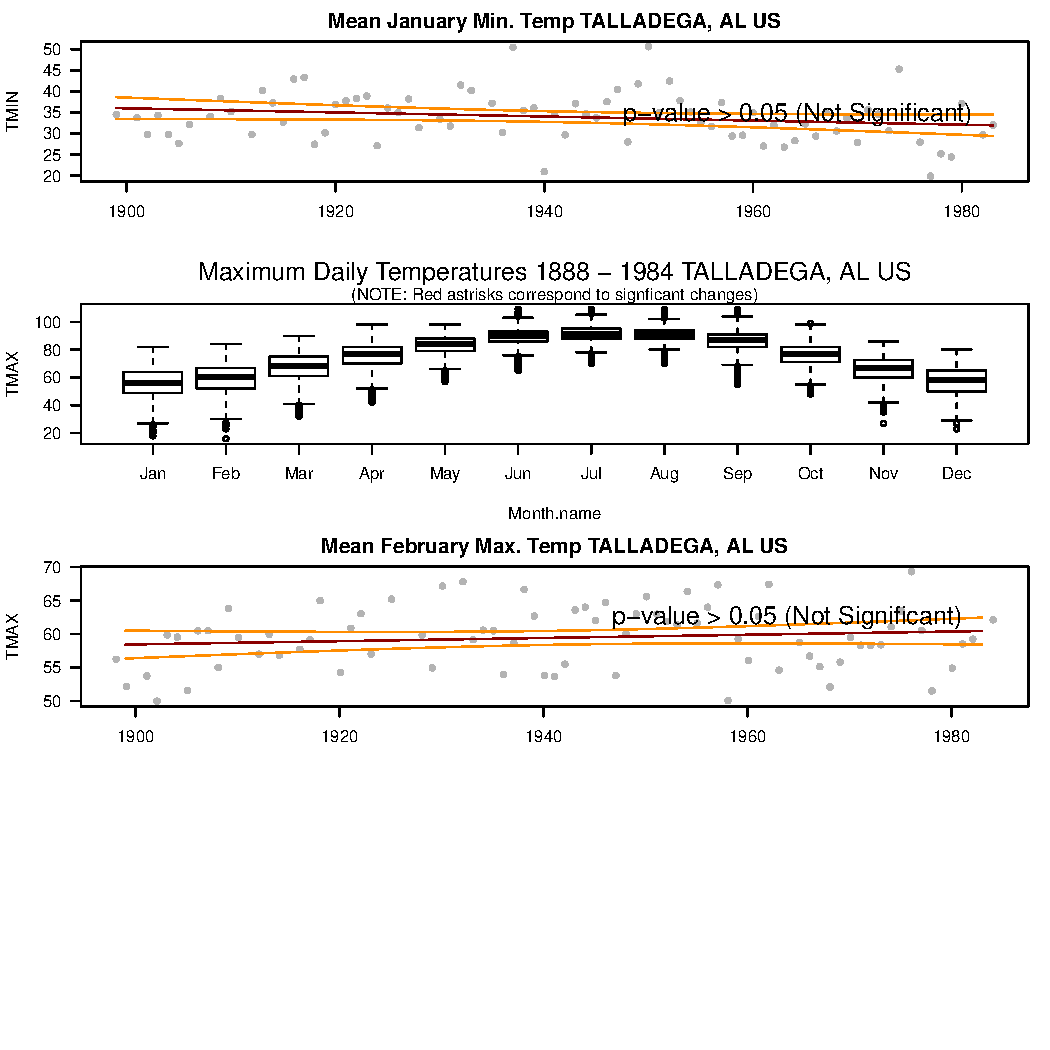
\includegraphics[width=\maxwidth]{figure/static_template-38} 

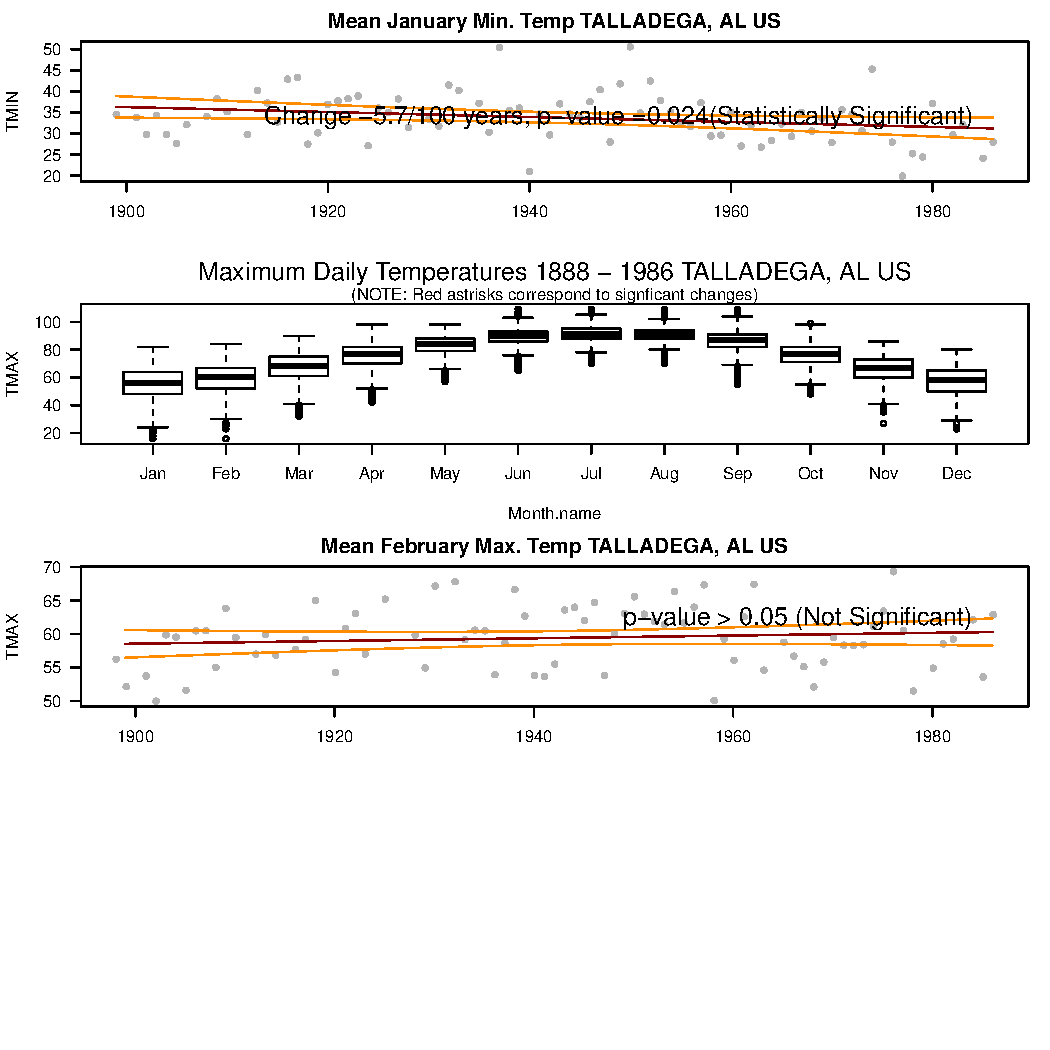
\includegraphics[width=\maxwidth]{figure/static_template-39} 

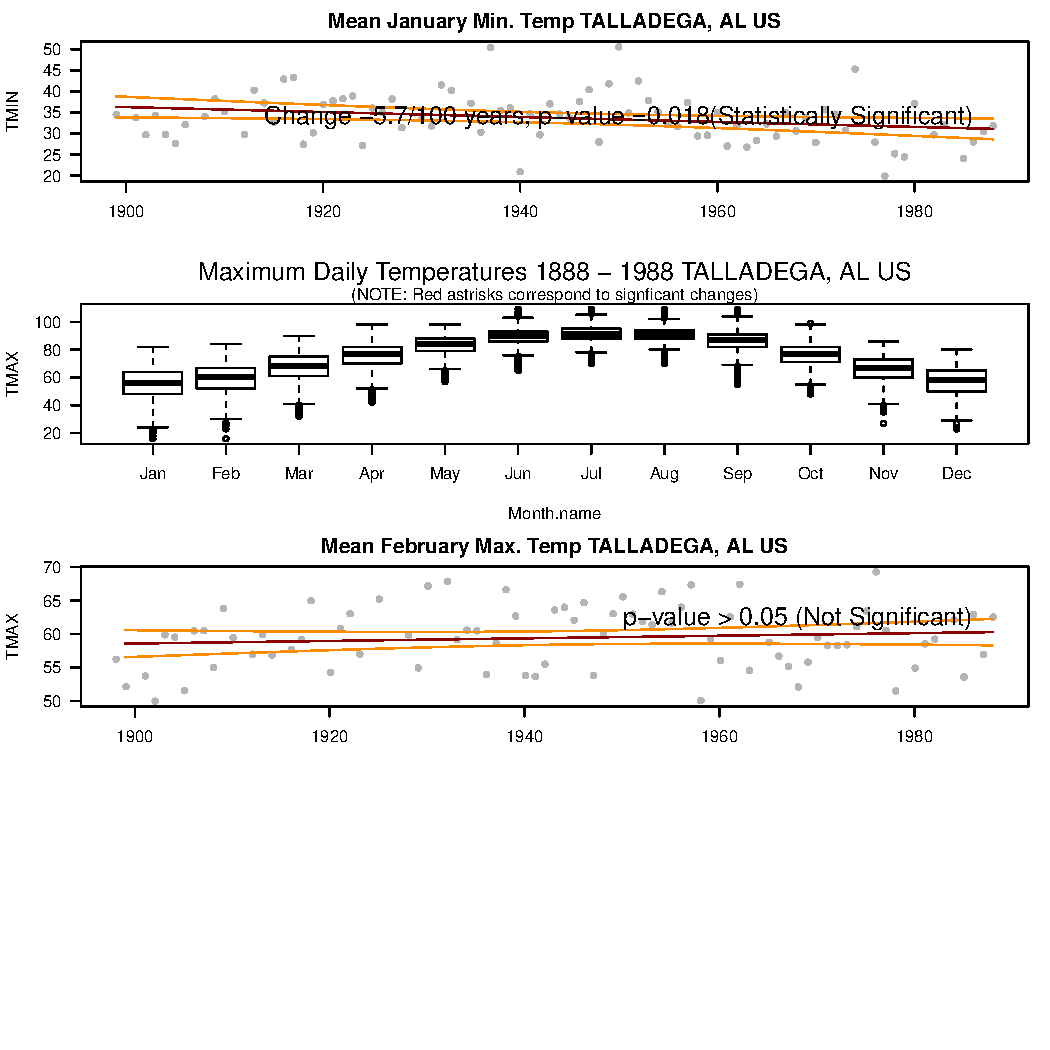
\includegraphics[width=\maxwidth]{figure/static_template-40} 

\includegraphics[width=\maxwidth]{figure/static_template-41} 

\includegraphics[width=\maxwidth]{figure/static_template-42} 

\includegraphics[width=\maxwidth]{figure/static_template-43} 

\includegraphics[width=\maxwidth]{figure/static_template-44} 

\includegraphics[width=\maxwidth]{figure/static_template-45} 

\includegraphics[width=\maxwidth]{figure/static_template-46} 

\includegraphics[width=\maxwidth]{figure/static_template-47} 

\includegraphics[width=\maxwidth]{figure/static_template-48} 

\includegraphics[width=\maxwidth]{figure/static_template-49} 

\includegraphics[width=\maxwidth]{figure/static_template-50} 

\includegraphics[width=\maxwidth]{figure/static_template-51} 

\includegraphics[width=\maxwidth]{figure/static_template-52} 

\includegraphics[width=\maxwidth]{figure/static_template-53} 

\includegraphics[width=\maxwidth]{figure/static_template-54} 

\includegraphics[width=\maxwidth]{figure/static_template-55} 

\includegraphics[width=\maxwidth]{figure/static_template-56} 
\begin{kframe}\begin{verbatim}
## null device 
##           1
\end{verbatim}
\end{kframe}
\end{knitrout}

\begin{figure}
\includegraphics[width=1.00\textwidth]{/home/CAMPUS/mwl04747/github/Climate_Change_Narratives/Social_Media/png/Alabama-USC00018024-GSOM.png}
\caption{Climate can be analyzed using several types of lenses. In this case, we have analyzed show the months with the greatest changes. The first figure is monthly average of TMINs (daily low temperatures) with a best fit line. The second figure shows the monthly TMAX range and asterisks indicate singificant changes over the station record and the third figure is the trend for these TMAXs over time and includes the best fit line. The final figure shows the daily temperatures that have been the highest on record (in red). In some cases, climate change has created more records in the recent decades, while other stations seem don't show that trend.}
\label{fig:GSOM}
\end{figure}

\subsection{KISS}

Keeping it simple is critical in communicating scientific information. In this section, I try to come up with a consistent message for every state and a simple graphic. 

\subsubsection{Change Point Analysis}
First, TMIN and TMAX and change point analysis...

https://cran.r-project.org/web/packages/mcp/readme/README.html

\begin{knitrout}
\definecolor{shadecolor}{rgb}{0.969, 0.969, 0.969}\color{fgcolor}\begin{kframe}
\begin{alltt}
\hlkwd{dyn.load}\hlstd{(}\hlstr{'/opt/jags/4.3.1/lib/libjags.so.4'}\hlstd{)}
\hlkwd{dyn.load}\hlstd{(}\hlstr{'/opt/jags/3.6/lib/libjags.so.4'}\hlstd{)}
\hlkwd{library}\hlstd{(mcp)}

\hlcom{# Define the model}
\hlstd{model} \hlkwb{=} \hlkwd{list}\hlstd{(}
  \hlstd{response} \hlopt{~} \hlnum{1}\hlstd{,}  \hlcom{# plateau (int_1)}
  \hlopt{~} \hlnum{0} \hlopt{+} \hlstd{time,}    \hlcom{# joined slope (time_2) at cp_1}
  \hlopt{~} \hlnum{1} \hlopt{+} \hlstd{time}     \hlcom{# disjoined slope (int_3, time_3) at cp_2}
\hlstd{)}

\hlcom{# Get example data and fit it}
\hlstd{ex} \hlkwb{=} \hlkwd{mcp_example}\hlstd{(}\hlstr{"demo"}\hlstd{)}
\hlstd{fit} \hlkwb{=} \hlkwd{mcp}\hlstd{(model,} \hlkwc{data} \hlstd{= ex}\hlopt{$}\hlstd{data)}


\hlkwd{dyn.load}\hlstd{(}\hlstr{'/opt/jags/4.3.1/lib/libjags.so.4'}\hlstd{)}
\hlkwd{library}\hlstd{(mcp)}
\hlcom{# library(rlang)}

\hlcom{# Simulate}
\hlkwd{set.seed}\hlstd{(}\hlnum{42}\hlstd{)}  \hlcom{# I always use 42; no fiddling}
\hlstd{df} \hlkwb{=} \hlkwd{data.frame}\hlstd{(}
  \hlkwc{x} \hlstd{=} \hlnum{1}\hlopt{:}\hlnum{100}\hlstd{,}
  \hlkwc{y} \hlstd{=} \hlkwd{c}\hlstd{(}\hlkwd{rnorm}\hlstd{(}\hlnum{30}\hlstd{,} \hlnum{2}\hlstd{),} \hlkwd{rnorm}\hlstd{(}\hlnum{40}\hlstd{,} \hlnum{0}\hlstd{),} \hlkwd{rnorm}\hlstd{(}\hlnum{30}\hlstd{,} \hlnum{1}\hlstd{))}
\hlstd{)}

\hlcom{# Plot it}
\hlkwd{plot}\hlstd{(df)}
\hlkwd{abline}\hlstd{(}\hlkwc{v} \hlstd{=} \hlkwd{c}\hlstd{(}\hlnum{30}\hlstd{,} \hlnum{70}\hlstd{),} \hlkwc{col}\hlstd{=}\hlstr{"red"}\hlstd{)}

\hlstd{model} \hlkwb{=} \hlkwd{list}\hlstd{(y}\hlopt{~}\hlnum{1}\hlstd{,} \hlnum{1}\hlopt{~}\hlnum{1}\hlstd{,} \hlnum{1}\hlopt{~}\hlnum{1}\hlstd{)}  \hlcom{# three intercept-only segments}
\hlstd{fit_mcp} \hlkwb{=} \hlkwd{mcp}\hlstd{(model,} \hlkwc{data} \hlstd{= df,} \hlkwc{par_x} \hlstd{=} \hlstr{"x"}\hlstd{)}

\hlkwd{summary}\hlstd{(fit_mcp)}

\hlkwd{library}\hlstd{(patchwork)}
\hlkwd{plot}\hlstd{(fit_mcp)} \hlopt{+} \hlkwd{plot_pars}\hlstd{(fit_mcp,} \hlkwc{pars} \hlstd{=} \hlkwd{c}\hlstd{(}\hlstr{"cp_1"}\hlstd{,} \hlstr{"cp_2"}\hlstd{),} \hlkwc{type} \hlstd{=} \hlstr{"dens_overlay"}\hlstd{)}

\hlstd{model} \hlkwb{=} \hlkwd{list}\hlstd{(}
  \hlstd{price} \hlopt{~} \hlnum{1} \hlopt{+} \hlkwd{ar}\hlstd{(}\hlnum{2}\hlstd{),}
  \hlopt{~} \hlnum{0} \hlopt{+} \hlstd{time} \hlopt{+} \hlkwd{ar}\hlstd{(}\hlnum{1}\hlstd{)}
\hlstd{)}
\hlstd{ex} \hlkwb{=} \hlkwd{mcp_example}\hlstd{(}\hlstr{"ar"}\hlstd{)}
\hlstd{fit} \hlkwb{=} \hlkwd{mcp}\hlstd{(model, ex}\hlopt{$}\hlstd{data)}
\hlkwd{summary}\hlstd{(fit)}
\end{alltt}
\end{kframe}
\end{knitrout}

Let's create a figure that simplifies the narrative, if we can!

\begin{knitrout}
\definecolor{shadecolor}{rgb}{0.969, 0.969, 0.969}\color{fgcolor}\begin{kframe}
\begin{verbatim}
## pdf 
##   2
\end{verbatim}
\end{kframe}
\end{knitrout}

\begin{figure}
\includegraphics[width=1.00\textwidth]{/home/CAMPUS/mwl04747/github/Climate_Change_Narratives/Social_Media/png/Alabama-USC00018024-KISS.png}
\caption{Keep it simple stupid!}
\label{fig:GSOM-KISS}
\end{figure}



\subsection{Temp \& Precipitation Probability}

To highlight the patterns of change, it might be useful to analyze how the probability ditributuion might change -- we can use a normal probability distribion as a theoretical distribution (and we can check if this distribuion is approrpriate with a Chi-Square test), or we can use the data to create a emperical distribution, which is my favored approach. 

I started with decade bins, but used 20 years bins (scores) to simplify the graphics while keeping a pretty good temporal resolution.

\begin{knitrout}
\definecolor{shadecolor}{rgb}{0.969, 0.969, 0.969}\color{fgcolor}\begin{kframe}
\begin{alltt}
\hlkwd{library}\hlstd{(wesanderson)}

\hlstd{h.ramp} \hlkwb{<-} \hlkwd{rev}\hlstd{(}\hlkwd{heat.colors}\hlstd{(}\hlkwd{length}\hlstd{(}\hlkwd{unique}\hlstd{(GSOM2}\hlopt{$}\hlstd{Score))}\hlopt{+}\hlnum{1}\hlstd{))[}\hlopt{-}\hlnum{1}\hlstd{]}
\hlstd{h.ramp} \hlkwb{<-} \hlkwd{wes_palette}\hlstd{(}\hlstr{"Zissou1"}\hlstd{,} \hlkwd{length}\hlstd{(}\hlkwd{unique}\hlstd{(GSOM2}\hlopt{$}\hlstd{Score)),}
      \hlkwc{type} \hlstd{=} \hlstr{"continuous"}\hlstd{)[}\hlnum{1}\hlopt{:}\hlkwd{length}\hlstd{(}\hlkwd{unique}\hlstd{(GSOM2}\hlopt{$}\hlstd{Score))]}
\hlcom{#TMAX.anomaly.Score = aggregate(TMAX.anom ~ Score, GSOM2, mean)}
\hlcom{#TMAX.sd.anomaly.Score = aggregate(TMAX.anom ~ Score, GSOM2, sd)}


\hlcom{# I hate list!}
\hlstd{TMAX.anomaly.list} \hlkwb{=} \hlkwd{aggregate}\hlstd{(TMAX.anom} \hlopt{~} \hlstd{Score, GSOM2,}
   \hlkwc{FUN} \hlstd{=} \hlkwa{function}\hlstd{(}\hlkwc{x}\hlstd{)} \hlkwd{c}\hlstd{(}\hlkwc{mean} \hlstd{=} \hlkwd{mean}\hlstd{(x),} \hlkwc{sd} \hlstd{=} \hlkwd{sd}\hlstd{(x)))}
\hlstd{TMIN.anomaly.list} \hlkwb{=} \hlkwd{aggregate}\hlstd{(TMIN.anom} \hlopt{~} \hlstd{Score, GSOM2,}
   \hlkwc{FUN} \hlstd{=} \hlkwa{function}\hlstd{(}\hlkwc{x}\hlstd{)} \hlkwd{c}\hlstd{(}\hlkwc{mean} \hlstd{=} \hlkwd{mean}\hlstd{(x),} \hlkwc{sd} \hlstd{=} \hlkwd{sd}\hlstd{(x)))}
\hlstd{PPT.anomaly.list} \hlkwb{=} \hlkwd{aggregate}\hlstd{(PPT.anom} \hlopt{~} \hlstd{Score, GSOM2,}
   \hlkwc{FUN} \hlstd{=} \hlkwa{function}\hlstd{(}\hlkwc{x}\hlstd{)} \hlkwd{c}\hlstd{(}\hlkwc{mean} \hlstd{=} \hlkwd{mean}\hlstd{(x),} \hlkwc{sd} \hlstd{=} \hlkwd{sd}\hlstd{(x)))}


\hlkwd{setwd}\hlstd{(}\hlstr{"/home/CAMPUS/mwl04747/github/Climate_Change_Narratives/Social_Media"}\hlstd{)}
\hlkwd{png}\hlstd{(}\hlkwd{paste0}\hlstd{(}\hlstr{"png//"}\hlstd{, fips}\hlopt{$}\hlstd{State,} \hlstr{"-"}\hlstd{, stid,} \hlstr{"-GSOM-normalPDF.png"}\hlstd{),}
    \hlkwc{width} \hlstd{=} \hlnum{480}\hlstd{,} \hlkwc{height} \hlstd{=} \hlnum{480}\hlstd{,} \hlkwc{units} \hlstd{=} \hlstr{"px"}\hlstd{,} \hlkwc{pointsize} \hlstd{=} \hlnum{12}\hlstd{,} \hlkwc{bg} \hlstd{=} \hlstr{"white"}\hlstd{)}
\hlcom{# TMIN}
\hlkwd{par}\hlstd{(}\hlkwc{mfrow}\hlstd{=}\hlkwd{c}\hlstd{(}\hlnum{2}\hlstd{,}\hlnum{2}\hlstd{),} \hlkwc{las}\hlstd{=}\hlnum{1}\hlstd{)}
\hlstd{Anom.x} \hlkwb{=} \hlkwd{seq}\hlstd{(}\hlkwd{min}\hlstd{(GSOM2}\hlopt{$}\hlstd{TMIN.anom),} \hlkwd{max}\hlstd{(GSOM2}\hlopt{$}\hlstd{TMIN.anom),}\hlkwc{by}\hlstd{=}\hlnum{.1}\hlstd{)}
\hlstd{Anom.y} \hlkwb{=} \hlkwd{max}\hlstd{(}\hlkwd{dnorm}\hlstd{(Anom.x,}
   \hlkwc{mean}\hlstd{=TMIN.anomaly.list}\hlopt{$}\hlstd{TMIN.anom[}\hlnum{1}\hlstd{,}\hlnum{1}\hlstd{],}
   \hlkwc{sd}\hlstd{=TMIN.anomaly.list}\hlopt{$}\hlstd{TMIN.anom[}\hlnum{1}\hlstd{,}\hlnum{2}\hlstd{]))}\hlopt{*}\hlnum{1.2}

\hlkwd{plot}\hlstd{(Anom.x,} \hlkwd{dnorm}\hlstd{(Anom.x,}
   \hlkwc{mean}\hlstd{=TMIN.anomaly.list}\hlopt{$}\hlstd{TMIN.anom[}\hlnum{1}\hlstd{,} \hlnum{1}\hlstd{],}
   \hlkwc{sd}\hlstd{=TMIN.anomaly.list}\hlopt{$}\hlstd{TMIN.anom[}\hlnum{1}\hlstd{,} \hlnum{2}\hlstd{]),}
   \hlkwc{ty}\hlstd{=}\hlstr{"l"}\hlstd{,} \hlkwc{col}\hlstd{=h.ramp[}\hlnum{1}\hlstd{],} \hlkwc{ylim}\hlstd{=}\hlkwd{c}\hlstd{(}\hlnum{0}\hlstd{, Anom.y),}
   \hlkwc{ylab}\hlstd{=}\hlstr{"Density"}\hlstd{,} \hlkwc{xlab}\hlstd{=}\hlstr{"TMIN Anomaly (°F)"}\hlstd{,} \hlkwc{main}\hlstd{=}\hlstr{""}\hlstd{)}

\hlkwd{abline}\hlstd{(}\hlkwc{v}\hlstd{=TMIN.anomaly.list}\hlopt{$}\hlstd{TMIN.anom[}\hlnum{1}\hlstd{,}\hlnum{1}\hlstd{],} \hlkwc{col}\hlstd{=h.ramp[}\hlnum{1}\hlstd{],} \hlkwc{lwd}\hlstd{=}\hlnum{2}\hlstd{)}
\hlkwa{for}\hlstd{(i} \hlkwa{in} \hlnum{2}\hlopt{:}\hlkwd{nrow}\hlstd{(TMIN.anomaly.list))\{}
\hlkwd{lines}\hlstd{(Anom.x,} \hlkwd{dnorm}\hlstd{(Anom.x,}
   \hlkwc{mean}\hlstd{=TMIN.anomaly.list}\hlopt{$}\hlstd{TMIN.anom[i,} \hlnum{1}\hlstd{],}
   \hlkwc{sd}\hlstd{=TMIN.anomaly.list}\hlopt{$}\hlstd{TMIN.anom[i,} \hlnum{2}\hlstd{]),} \hlkwc{col}\hlstd{=h.ramp[i])}
\hlstd{\}}
\hlkwd{abline}\hlstd{(}\hlkwc{v}\hlstd{=TMIN.anomaly.list}\hlopt{$}\hlstd{TMIN.anom[i,}\hlnum{1}\hlstd{],} \hlkwc{col}\hlstd{=h.ramp[i],} \hlkwc{lwd}\hlstd{=}\hlnum{2}\hlstd{)}
\hlstd{Delta} \hlkwb{=} \hlstd{TMIN.anomaly.list}\hlopt{$}\hlstd{TMIN.anom[i,}\hlnum{1}\hlstd{]} \hlopt{-} \hlstd{TMIN.anomaly.list}\hlopt{$}\hlstd{TMIN.anom[}\hlnum{1}\hlstd{,}\hlnum{1}\hlstd{]}

\hlkwd{text}\hlstd{(TMIN.anomaly.list}\hlopt{$}\hlstd{TMIN.anom[i,}\hlnum{1}\hlstd{], Anom.y}\hlopt{*}\hlnum{.9}\hlstd{,}
   \hlkwd{paste0}\hlstd{(}\hlstr{"Change "}\hlstd{,} \hlkwd{round}\hlstd{(Delta,} \hlnum{1}\hlstd{),} \hlstr{"°F"}\hlstd{),} \hlkwc{pos}\hlstd{=}\hlnum{4}\hlstd{)}

\hlkwd{mtext}\hlstd{(}\hlkwd{paste0}\hlstd{(fips}\hlopt{$}\hlstd{State,} \hlstr{" ("}\hlstd{, GSOM_Longest}\hlopt{$}\hlstd{name,} \hlstr{")"}\hlstd{),} \hlkwc{side}\hlstd{=}\hlnum{3}\hlstd{,} \hlkwc{line}\hlstd{=}\hlnum{2}\hlstd{)}

\hlcom{# TMAX}
\hlstd{Anom.x} \hlkwb{=} \hlkwd{seq}\hlstd{(}\hlkwd{min}\hlstd{(GSOM2}\hlopt{$}\hlstd{TMAX.anom),} \hlkwd{max}\hlstd{(GSOM2}\hlopt{$}\hlstd{TMAX.anom),}\hlkwc{by}\hlstd{=}\hlnum{.1}\hlstd{)}
\hlstd{Anom.y} \hlkwb{=} \hlkwd{max}\hlstd{(}\hlkwd{dnorm}\hlstd{(Anom.x,}
   \hlkwc{mean}\hlstd{=TMAX.anomaly.list}\hlopt{$}\hlstd{TMAX.anom[}\hlnum{1}\hlstd{,}\hlnum{1}\hlstd{],}
   \hlkwc{sd}\hlstd{=TMAX.anomaly.list}\hlopt{$}\hlstd{TMAX.anom[}\hlnum{1}\hlstd{,}\hlnum{2}\hlstd{]))}\hlopt{*}\hlnum{1.2}

\hlkwd{plot}\hlstd{(Anom.x,} \hlkwd{dnorm}\hlstd{(Anom.x,}
   \hlkwc{mean}\hlstd{=TMAX.anomaly.list}\hlopt{$}\hlstd{TMAX.anom[}\hlnum{1}\hlstd{,} \hlnum{1}\hlstd{],}
   \hlkwc{sd}\hlstd{=TMAX.anomaly.list}\hlopt{$}\hlstd{TMAX.anom[}\hlnum{1}\hlstd{,} \hlnum{2}\hlstd{]),}
   \hlkwc{ty}\hlstd{=}\hlstr{"l"}\hlstd{,} \hlkwc{col}\hlstd{=h.ramp[}\hlnum{1}\hlstd{],} \hlkwc{ylim}\hlstd{=}\hlkwd{c}\hlstd{(}\hlnum{0}\hlstd{, Anom.y),}
   \hlkwc{ylab}\hlstd{=}\hlstr{"Density"}\hlstd{,} \hlkwc{xlab}\hlstd{=}\hlstr{"TMAX Anomaly (°F)"}\hlstd{)}

\hlkwd{abline}\hlstd{(}\hlkwc{v}\hlstd{=TMAX.anomaly.list}\hlopt{$}\hlstd{TMAX.anom[}\hlnum{1}\hlstd{,}\hlnum{1}\hlstd{],} \hlkwc{col}\hlstd{=h.ramp[}\hlnum{1}\hlstd{],} \hlkwc{lwd}\hlstd{=}\hlnum{2}\hlstd{)}
\hlkwa{for}\hlstd{(i} \hlkwa{in} \hlnum{2}\hlopt{:}\hlkwd{nrow}\hlstd{(TMAX.anomaly.list))\{}
\hlkwd{lines}\hlstd{(Anom.x,} \hlkwd{dnorm}\hlstd{(Anom.x,}
   \hlkwc{mean}\hlstd{=TMAX.anomaly.list}\hlopt{$}\hlstd{TMAX.anom[i,} \hlnum{1}\hlstd{],}
   \hlkwc{sd}\hlstd{=TMAX.anomaly.list}\hlopt{$}\hlstd{TMAX.anom[i,} \hlnum{2}\hlstd{]),} \hlkwc{col}\hlstd{=h.ramp[i])}
\hlstd{\}}
\hlkwd{abline}\hlstd{(}\hlkwc{v}\hlstd{=TMAX.anomaly.list}\hlopt{$}\hlstd{TMAX.anom[i,}\hlnum{1}\hlstd{],} \hlkwc{col}\hlstd{=h.ramp[i],} \hlkwc{lwd}\hlstd{=}\hlnum{2}\hlstd{)}
\hlstd{Delta} \hlkwb{=} \hlstd{TMAX.anomaly.list}\hlopt{$}\hlstd{TMAX.anom[i,}\hlnum{1}\hlstd{]} \hlopt{-} \hlstd{TMAX.anomaly.list}\hlopt{$}\hlstd{TMAX.anom[}\hlnum{1}\hlstd{,}\hlnum{1}\hlstd{]}

\hlkwd{text}\hlstd{(TMAX.anomaly.list}\hlopt{$}\hlstd{TMAX.anom[i,}\hlnum{1}\hlstd{], Anom.y}\hlopt{*}\hlnum{.9}\hlstd{,}
   \hlkwd{paste0}\hlstd{(}\hlstr{"Change "}\hlstd{,} \hlkwd{round}\hlstd{(Delta,} \hlnum{1}\hlstd{),} \hlstr{"°F"}\hlstd{),} \hlkwc{pos}\hlstd{=}\hlnum{4}\hlstd{)}

\hlcom{# PPT}
\hlstd{Anom.x} \hlkwb{=} \hlkwd{seq}\hlstd{(}\hlkwd{min}\hlstd{(GSOM2}\hlopt{$}\hlstd{PPT.anom),} \hlkwd{max}\hlstd{(GSOM2}\hlopt{$}\hlstd{PPT.anom),}\hlkwc{by}\hlstd{=}\hlnum{.1}\hlstd{)}
\hlstd{Anom.y} \hlkwb{=} \hlkwd{max}\hlstd{(}\hlkwd{dnorm}\hlstd{(Anom.x,}
   \hlkwc{mean}\hlstd{=PPT.anomaly.list}\hlopt{$}\hlstd{PPT.anom[}\hlnum{1}\hlstd{,}\hlnum{1}\hlstd{],}
   \hlkwc{sd}\hlstd{=PPT.anomaly.list}\hlopt{$}\hlstd{PPT.anom[}\hlnum{1}\hlstd{,}\hlnum{2}\hlstd{]))}\hlopt{*}\hlnum{1.2}

\hlkwd{plot}\hlstd{(Anom.x,} \hlkwd{dnorm}\hlstd{(Anom.x,}
   \hlkwc{mean}\hlstd{=PPT.anomaly.list}\hlopt{$}\hlstd{PPT.anom[}\hlnum{1}\hlstd{,} \hlnum{1}\hlstd{],}
   \hlkwc{sd}\hlstd{=PPT.anomaly.list}\hlopt{$}\hlstd{PPT.anom[}\hlnum{1}\hlstd{,} \hlnum{2}\hlstd{]),}
   \hlkwc{ty}\hlstd{=}\hlstr{"l"}\hlstd{,} \hlkwc{col}\hlstd{=h.ramp[}\hlnum{1}\hlstd{],} \hlkwc{ylim}\hlstd{=}\hlkwd{c}\hlstd{(}\hlnum{0}\hlstd{, Anom.y),}
   \hlkwc{ylab}\hlstd{=}\hlstr{"Density"}\hlstd{,} \hlkwc{xlab}\hlstd{=}\hlstr{"PPT Anomaly"}\hlstd{)}

\hlkwd{abline}\hlstd{(}\hlkwc{v}\hlstd{=PPT.anomaly.list}\hlopt{$}\hlstd{PPT.anom[}\hlnum{1}\hlstd{,}\hlnum{1}\hlstd{],} \hlkwc{col}\hlstd{=h.ramp[}\hlnum{1}\hlstd{],} \hlkwc{lwd}\hlstd{=}\hlnum{2}\hlstd{)}
\hlkwa{for}\hlstd{(i} \hlkwa{in} \hlnum{2}\hlopt{:}\hlkwd{nrow}\hlstd{(PPT.anomaly.list))\{}
\hlkwd{lines}\hlstd{(Anom.x,} \hlkwd{dnorm}\hlstd{(Anom.x,}
   \hlkwc{mean}\hlstd{=PPT.anomaly.list}\hlopt{$}\hlstd{PPT.anom[i,} \hlnum{1}\hlstd{],}
   \hlkwc{sd}\hlstd{=PPT.anomaly.list}\hlopt{$}\hlstd{PPT.anom[i,} \hlnum{2}\hlstd{]),} \hlkwc{col}\hlstd{=h.ramp[i])}
\hlstd{\}}
\hlkwd{abline}\hlstd{(}\hlkwc{v}\hlstd{=PPT.anomaly.list}\hlopt{$}\hlstd{PPT.anom[i,}\hlnum{1}\hlstd{],} \hlkwc{col}\hlstd{=h.ramp[i],} \hlkwc{lwd}\hlstd{=}\hlnum{2}\hlstd{)}
\hlstd{Delta} \hlkwb{=} \hlstd{PPT.anomaly.list}\hlopt{$}\hlstd{PPT.anom[i,}\hlnum{1}\hlstd{]} \hlopt{-} \hlstd{PPT.anomaly.list}\hlopt{$}\hlstd{PPT.anom[}\hlnum{1}\hlstd{,}\hlnum{1}\hlstd{]}

\hlkwd{text}\hlstd{(PPT.anomaly.list}\hlopt{$}\hlstd{PPT.anom[i,}\hlnum{1}\hlstd{], Anom.y}\hlopt{*}\hlnum{.9}\hlstd{,}
   \hlkwd{paste0}\hlstd{(}\hlstr{"Change "}\hlstd{,} \hlkwd{round}\hlstd{(Delta,} \hlnum{1}\hlstd{),} \hlstr{" inches"}\hlstd{),} \hlkwc{pos}\hlstd{=}\hlnum{4}\hlstd{)}

\hlkwd{dev.off}\hlstd{()}
\end{alltt}
\begin{verbatim}
## pdf 
##   2
\end{verbatim}
\end{kframe}
\end{knitrout}

This figure is pretty effective, but still needs work. 

\begin{figure}
\includegraphics[width=1.00\textwidth]{/home/CAMPUS/mwl04747/github/Climate_Change_Narratives/Social_Media/png/Alabama-USC00018024-GSOM-normalPDF.png}
\caption{The changing in monthly temperature data, assuming a normal probability distribution.}
\label{fig:GSOM-normalPDF}
\end{figure}

\subsection{Using library densEstBayes}

Now, I used a screen split to look at the distribution of the temperate anomolies. First, we look at a simple histogram of the entire dataset. 

\begin{knitrout}
\definecolor{shadecolor}{rgb}{0.969, 0.969, 0.969}\color{fgcolor}\begin{kframe}
\begin{alltt}
\hlkwd{par}\hlstd{(}\hlkwc{mfrow}\hlstd{=}\hlkwd{c}\hlstd{(}\hlnum{1}\hlstd{,}\hlnum{1}\hlstd{))}
\hlkwd{hist}\hlstd{(GSOM2}\hlopt{$}\hlstd{TMIN.anom,} \hlkwc{col} \hlstd{=} \hlstr{"gold"}\hlstd{,}
     \hlkwc{main} \hlstd{=} \hlstr{""}\hlstd{,} \hlkwc{probability} \hlstd{=} \hlnum{TRUE}\hlstd{,}
     \hlkwc{xlab} \hlstd{=} \hlstr{"Minimum Temperature Anomaly (°F)"}\hlstd{)}
\end{alltt}
\end{kframe}
\includegraphics[width=\maxwidth]{figure/unnamed-chunk-16-1} 
\end{knitrout}

The data center around zero, as expected, but are these normally distributed? 

For TMAX there is a 0.031 probability that the distribution is the same as the normal distribution. For TMIN there is a 0 probability that the distribution is the same as the normal distribution. For PPT is a 0 probability that the distribution is the same as the normal distribution.

\begin{knitrout}
\definecolor{shadecolor}{rgb}{0.969, 0.969, 0.969}\color{fgcolor}\begin{kframe}
\begin{alltt}
\hlkwa{if}\hlstd{(}\hlkwd{shapiro.test}\hlstd{(GSOM2}\hlopt{$}\hlstd{TMAX.anom)}\hlopt{$}\hlstd{p.value}\hlopt{<}\hlnum{.05} \hlopt{|}
   \hlkwd{shapiro.test}\hlstd{(GSOM2}\hlopt{$}\hlstd{TMIN.anom)}\hlopt{$}\hlstd{p.value}\hlopt{<}\hlnum{.05} \hlopt{|}
   \hlkwd{shapiro.test}\hlstd{(GSOM2}\hlopt{$}\hlstd{PPT.anom)}\hlopt{$}\hlstd{p.value}\hlopt{<}\hlnum{.05}\hlstd{) text}\hlkwb{=}\hlstr{"to avoid "} \hlkwa{else} \hlstd{text}\hlkwb{=}\hlstr{"to use"}
\end{alltt}
\end{kframe}
\end{knitrout}

These values suggest that there is good reason to avoid  the normal probability distribution. 

Next we use a function to estimate the probability distribution using a markof chain the creates an estimated probability distribution. This doesn't always work when the distribution is not even and their only 10 years of data per slot. I suspect, I should make this by every 20 years. Plus that will go way faster and I think the data visualization will be more robust. 

\begin{knitrout}
\definecolor{shadecolor}{rgb}{0.969, 0.969, 0.969}\color{fgcolor}\begin{kframe}
\begin{alltt}
\hlkwd{setwd}\hlstd{(}\hlstr{"/home/CAMPUS/mwl04747/github/Climate_Change_Narratives/Social_Media"}\hlstd{)}

\hlkwa{if}\hlstd{(}\hlopt{!}\hlkwd{file.exists}\hlstd{(}\hlkwd{paste0}\hlstd{(}\hlstr{"png//"}\hlstd{, fips}\hlopt{$}\hlstd{State,} \hlstr{"-"}\hlstd{, stid,} \hlstr{"-GSOM-estDensity.png"}\hlstd{)))\{}
   \hlkwd{print}\hlstd{(}\hlstr{"Creating estimated density distribution"}\hlstd{)}

\hlkwd{png}\hlstd{(}\hlkwd{paste0}\hlstd{(}\hlstr{"png//"}\hlstd{, fips}\hlopt{$}\hlstd{State,} \hlstr{"-"}\hlstd{, stid,} \hlstr{"-GSOM-estDensity.png"}\hlstd{),}
    \hlkwc{width} \hlstd{=} \hlnum{480}\hlstd{,} \hlkwc{height} \hlstd{=} \hlnum{320}\hlstd{,} \hlkwc{units} \hlstd{=} \hlstr{"px"}\hlstd{,} \hlkwc{pointsize} \hlstd{=} \hlnum{12}\hlstd{,} \hlkwc{bg} \hlstd{=} \hlstr{"white"}\hlstd{)}

\hlcom{# Split Screen TMAX Legend TMIN}
\hlcom{# screen with values for left, right, bottom, and top.}
\hlkwd{split.screen}\hlstd{(}\hlkwd{rbind}\hlstd{(}\hlkwd{c}\hlstd{(}\hlnum{.01}\hlstd{,} \hlnum{0.99}\hlstd{,} \hlnum{0.86}\hlstd{,} \hlnum{0.95}\hlstd{),}
                   \hlkwd{c}\hlstd{(}\hlnum{0.01}\hlstd{,} \hlnum{0.45}\hlstd{,} \hlnum{0.01}\hlstd{,} \hlnum{0.85}\hlstd{),}
                   \hlkwd{c}\hlstd{(}\hlnum{0.45}\hlstd{,} \hlnum{0.55}\hlstd{,} \hlnum{0.01}\hlstd{,} \hlnum{0.85}\hlstd{),}
                   \hlkwd{c}\hlstd{(}\hlnum{0.55}\hlstd{,} \hlnum{0.99}\hlstd{,} \hlnum{0.01}\hlstd{,} \hlnum{0.85}\hlstd{)))}

\hlkwd{screen}\hlstd{(}\hlnum{1}\hlstd{)}
\hlkwd{par}\hlstd{(}\hlkwc{mar}\hlstd{=}\hlkwd{c}\hlstd{(}\hlnum{0}\hlstd{,}\hlnum{0}\hlstd{,}\hlnum{0}\hlstd{,}\hlnum{0}\hlstd{))}
\hlkwd{plot}\hlstd{(}\hlnum{NA}\hlstd{,} \hlkwc{xaxt}\hlstd{=}\hlstr{'n'}\hlstd{,}\hlkwc{yaxt}\hlstd{=}\hlstr{'n'}\hlstd{,}\hlkwc{bty}\hlstd{=}\hlstr{'n'}\hlstd{,}\hlkwc{ylab}\hlstd{=}\hlstr{''}\hlstd{,}\hlkwc{xlab}\hlstd{=}\hlstr{''}\hlstd{,} \hlkwc{xlim}\hlstd{=}\hlkwd{c}\hlstd{(}\hlnum{0}\hlstd{,}\hlnum{10}\hlstd{),} \hlkwc{ylim}\hlstd{=}\hlkwd{c}\hlstd{(}\hlnum{0}\hlstd{,} \hlnum{10}\hlstd{))}
\hlkwd{mtext}\hlstd{(}\hlkwd{paste0}\hlstd{(fips}\hlopt{$}\hlstd{State,} \hlstr{" ("}\hlstd{, GSOM_Longest}\hlopt{$}\hlstd{name,} \hlstr{")"}\hlstd{),} \hlkwc{side}\hlstd{=}\hlnum{3}\hlstd{,} \hlkwc{line}\hlstd{=}\hlopt{-}\hlnum{1}\hlstd{,} \hlkwc{cex}\hlstd{=}\hlnum{1.4}\hlstd{)}

\hlkwd{screen}\hlstd{(}\hlnum{2}\hlstd{)}

\hlcom{# Determine xg (range)}
\hlstd{dest} \hlkwb{<-} \hlkwd{densEstBayes}\hlstd{(GSOM2}\hlopt{$}\hlstd{TMIN.anom,} \hlkwc{method} \hlstd{=} \hlstr{"NUTS"}\hlstd{); dest}\hlopt{$}\hlstd{range.x}

\hlstd{control} \hlkwb{=} \hlkwd{densEstBayes.control}\hlstd{(}\hlkwc{range.x} \hlstd{= dest}\hlopt{$}\hlstd{range.x,}
      \hlkwc{numBins} \hlstd{=} \hlnum{401}\hlstd{,}
      \hlkwc{numBasis} \hlstd{=} \hlnum{50}\hlstd{,} \hlkwc{sigmabeta} \hlstd{=} \hlnum{1e5}\hlstd{,} \hlkwc{ssigma} \hlstd{=} \hlnum{1000}\hlstd{,}
      \hlkwc{convToler} \hlstd{=} \hlnum{1e-5}\hlstd{,} \hlkwc{maxIter} \hlstd{=} \hlnum{500}\hlstd{,} \hlkwc{nWarm} \hlstd{=} \hlkwa{NULL}\hlstd{,}
      \hlkwc{nKept} \hlstd{=} \hlkwa{NULL}\hlstd{,} \hlkwc{nThin} \hlstd{=} \hlnum{1}\hlstd{,} \hlkwc{msgCode} \hlstd{=} \hlnum{1}\hlstd{)}

\hlcom{#destSMFVB <- densEstBayes(GSOM2$TMIN.anom, method = "SMFVB", control = control)}
\hlcom{#plot(destSMFVB, plotIt=T, xlab = "TMIN", main = "", setCol=h.ramp[i])}
\hlkwd{par}\hlstd{(}\hlkwc{las}\hlstd{=}\hlnum{1}\hlstd{,} \hlkwc{mar}\hlstd{=}\hlkwd{c}\hlstd{(}\hlnum{4}\hlstd{,} \hlnum{4}\hlstd{,} \hlnum{0}\hlstd{,} \hlnum{0}\hlstd{)} \hlopt{+} \hlnum{0.1}\hlstd{)}
\hlkwa{for}\hlstd{(i} \hlkwa{in} \hlnum{1}\hlopt{:}\hlkwd{length}\hlstd{(}\hlkwd{unique}\hlstd{(GSOM2}\hlopt{$}\hlstd{Score)))\{}
   \hlcom{# i = 13}
   \hlstd{GSOM2sub} \hlkwb{=} \hlstd{GSOM2[GSOM2}\hlopt{$}\hlstd{Score}\hlopt{==}\hlkwd{sort}\hlstd{(}\hlkwd{unique}\hlstd{(GSOM2}\hlopt{$}\hlstd{Score))[i],]}
   \hlstd{dest} \hlkwb{<-} \hlkwd{densEstBayes}\hlstd{(GSOM2sub}\hlopt{$}\hlstd{TMIN.anom,} \hlkwc{method} \hlstd{=} \hlstr{"NUTS"}\hlstd{,} \hlkwc{control} \hlstd{= control)}
   \hlstd{xg} \hlkwb{=} \hlkwd{plot}\hlstd{(dest,} \hlkwc{plotIt}\hlstd{=}\hlnum{FALSE}\hlstd{)}\hlopt{$}\hlstd{xg}
   \hlstd{densEstg} \hlkwb{=} \hlkwd{plot}\hlstd{(dest,} \hlkwc{plotIt}\hlstd{=}\hlnum{FALSE}\hlstd{)}\hlopt{$}\hlstd{densEstg}

   \hlkwa{if}\hlstd{(i}\hlopt{==}\hlnum{1}\hlstd{)} \hlkwd{plot}\hlstd{(}\hlnum{0}\hlstd{,} \hlkwc{type} \hlstd{=} \hlstr{"n"}\hlstd{,} \hlkwc{bty} \hlstd{=} \hlstr{"l"}\hlstd{,}
         \hlkwc{xlim}\hlstd{=}\hlkwd{range}\hlstd{(xg),} \hlkwc{ylim}\hlstd{=}\hlkwd{c}\hlstd{(}\hlnum{0}\hlstd{,}\hlnum{0.25}\hlstd{),}
         \hlkwc{xlab} \hlstd{=} \hlstr{"TMIN anomaly (°F)"}\hlstd{,} \hlkwc{main} \hlstd{=} \hlstr{""}\hlstd{,} \hlkwc{ylab}\hlstd{=}\hlstr{"Density"}\hlstd{)}
   \hlkwd{lines}\hlstd{(xg, densEstg,} \hlkwc{col}\hlstd{=h.ramp[i])}
\hlkwd{rug}\hlstd{(}\hlkwd{jitter}\hlstd{(GSOM2sub}\hlopt{$}\hlstd{TMIN.anom,}\hlkwc{amount} \hlstd{=} \hlnum{0.2}\hlstd{),} \hlkwc{col}\hlstd{=h.ramp[i])}
\hlstd{\}}

\hlkwd{screen}\hlstd{(}\hlnum{3}\hlstd{)}
\hlkwd{par}\hlstd{(}\hlkwc{mar}\hlstd{=}\hlkwd{c}\hlstd{(}\hlnum{0}\hlstd{,}\hlnum{0}\hlstd{,}\hlnum{1}\hlstd{,}\hlnum{0}\hlstd{))}
\hlkwd{plot}\hlstd{(}\hlnum{NA}\hlstd{,}\hlkwc{xaxt}\hlstd{=}\hlstr{'n'}\hlstd{,}\hlkwc{yaxt}\hlstd{=}\hlstr{'n'}\hlstd{,}\hlkwc{bty}\hlstd{=}\hlstr{'n'}\hlstd{,}\hlkwc{ylab}\hlstd{=}\hlstr{''}\hlstd{,}\hlkwc{xlab}\hlstd{=}\hlstr{''}\hlstd{,} \hlkwc{xlim}\hlstd{=}\hlkwd{c}\hlstd{(}\hlnum{0}\hlstd{,}\hlnum{10}\hlstd{),} \hlkwc{ylim}\hlstd{=}\hlkwd{c}\hlstd{(}\hlnum{0}\hlstd{,}\hlnum{10}\hlstd{))}
\hlcom{# }
\hlkwd{legend}\hlstd{(}\hlstr{"topright"}\hlstd{,} \hlkwc{inset}\hlstd{=}\hlkwd{c}\hlstd{(}\hlnum{0}\hlstd{,}\hlnum{0}\hlstd{),} \hlkwc{bg}\hlstd{=}\hlstr{"transparent"}\hlstd{,} \hlkwc{bty}\hlstd{=}\hlstr{"n"}\hlstd{,}
       \hlkwc{legend}\hlstd{=}\hlkwd{unique}\hlstd{(GSOM2}\hlopt{$}\hlstd{Score),}
       \hlkwc{fill}\hlstd{=h.ramp,} \hlkwc{horiz}\hlstd{=}\hlnum{FALSE}\hlstd{,} \hlkwc{cex}\hlstd{=}\hlnum{0.85}\hlstd{)}

\hlkwd{screen}\hlstd{(}\hlnum{4}\hlstd{)}
\hlkwd{par}\hlstd{(}\hlkwc{las}\hlstd{=}\hlnum{1}\hlstd{,} \hlkwc{mar}\hlstd{=}\hlkwd{c}\hlstd{(}\hlnum{4}\hlstd{,} \hlnum{4}\hlstd{,} \hlnum{0}\hlstd{,} \hlnum{0}\hlstd{)} \hlopt{+}\hlnum{0.1}\hlstd{)}
\hlcom{# Determine xg (range)}
\hlstd{dest} \hlkwb{<-} \hlkwd{densEstBayes}\hlstd{(GSOM2}\hlopt{$}\hlstd{TMAX.anom,} \hlkwc{method} \hlstd{=} \hlstr{"NUTS"}\hlstd{); dest}\hlopt{$}\hlstd{range.x}

\hlstd{control} \hlkwb{=} \hlkwd{densEstBayes.control}\hlstd{(}\hlkwc{range.x} \hlstd{= dest}\hlopt{$}\hlstd{range.x,}
      \hlkwc{numBins} \hlstd{=} \hlnum{401}\hlstd{,}
      \hlkwc{numBasis} \hlstd{=} \hlnum{50}\hlstd{,} \hlkwc{sigmabeta} \hlstd{=} \hlnum{1e5}\hlstd{,} \hlkwc{ssigma} \hlstd{=} \hlnum{1000}\hlstd{,}
      \hlkwc{convToler} \hlstd{=} \hlnum{1e-5}\hlstd{,} \hlkwc{maxIter} \hlstd{=} \hlnum{500}\hlstd{,} \hlkwc{nWarm} \hlstd{=} \hlkwa{NULL}\hlstd{,}
      \hlkwc{nKept} \hlstd{=} \hlkwa{NULL}\hlstd{,} \hlkwc{nThin} \hlstd{=} \hlnum{1}\hlstd{,} \hlkwc{msgCode} \hlstd{=} \hlnum{1}\hlstd{)}

\hlkwa{for}\hlstd{(i} \hlkwa{in} \hlnum{1}\hlopt{:}\hlkwd{length}\hlstd{(}\hlkwd{unique}\hlstd{(GSOM2}\hlopt{$}\hlstd{Score)))\{}
   \hlcom{# i = 13}
   \hlstd{GSOM2sub} \hlkwb{=} \hlstd{GSOM2[GSOM2}\hlopt{$}\hlstd{Score}\hlopt{==}\hlkwd{sort}\hlstd{(}\hlkwd{unique}\hlstd{(GSOM2}\hlopt{$}\hlstd{Score))[i],]}
   \hlstd{dest} \hlkwb{<-} \hlkwd{densEstBayes}\hlstd{(GSOM2sub}\hlopt{$}\hlstd{TMAX.anom,} \hlkwc{method} \hlstd{=} \hlstr{"NUTS"}\hlstd{,} \hlkwc{control} \hlstd{= control)}
   \hlstd{xg} \hlkwb{=} \hlkwd{plot}\hlstd{(dest,} \hlkwc{plotIt}\hlstd{=}\hlnum{FALSE}\hlstd{)}\hlopt{$}\hlstd{xg}
   \hlstd{densEstg} \hlkwb{=} \hlkwd{plot}\hlstd{(dest,} \hlkwc{plotIt}\hlstd{=}\hlnum{FALSE}\hlstd{)}\hlopt{$}\hlstd{densEstg}

   \hlkwa{if}\hlstd{(i}\hlopt{==}\hlnum{1}\hlstd{)} \hlkwd{plot}\hlstd{(}\hlnum{0}\hlstd{,} \hlkwc{type} \hlstd{=} \hlstr{"n"}\hlstd{,} \hlkwc{bty} \hlstd{=} \hlstr{"l"}\hlstd{,}
         \hlkwc{xlim}\hlstd{=}\hlkwd{range}\hlstd{(xg),} \hlkwc{ylim}\hlstd{=}\hlkwd{c}\hlstd{(}\hlnum{0}\hlstd{,}\hlnum{.25}\hlstd{),}
         \hlkwc{xlab} \hlstd{=} \hlstr{"TMAX anomaly (°F)"}\hlstd{,} \hlkwc{main} \hlstd{=} \hlstr{""}\hlstd{,} \hlkwc{ylab}\hlstd{=}\hlstr{"Density"}\hlstd{)}
   \hlkwd{lines}\hlstd{(xg, densEstg,} \hlkwc{col}\hlstd{=h.ramp[i])}
\hlkwd{rug}\hlstd{(}\hlkwd{jitter}\hlstd{(GSOM2sub}\hlopt{$}\hlstd{TMIN.anom,}\hlkwc{amount} \hlstd{=} \hlnum{0.2}\hlstd{),} \hlkwc{col}\hlstd{=h.ramp[i])}
\hlstd{\}}
\hlcom{#rug(jitter(GSOM2sub$TMIN.anom,amount = 0.2), col=h.ramp[i])}

\hlkwd{close.screen}\hlstd{(}\hlkwc{all.screens} \hlstd{=} \hlnum{TRUE}\hlstd{)}
\hlkwd{dev.off}\hlstd{()}
\hlstd{\}} \hlkwa{else} \hlstd{\{}
   \hlkwd{print}\hlstd{(}\hlstr{"Skipping estimated density distribution chunk"}\hlstd{)\}}
\end{alltt}
\end{kframe}
\end{knitrout}

The process to create these figures is very time consuming, so in general, I need to come up with an if then statement to avoid creating these everytime!

\begin{figure}
\includegraphics[width=1.00\textwidth]{/home/CAMPUS/mwl04747/github/Climate_Change_Narratives/Social_Media/png/Alabama-USC00018024-GSOM-estDensity.png}
\caption{The changing in monthly temperature data.}
\label{fig:GSOM-estDensity}
\end{figure}

\section{Animated GIFs}

So far, this creates a gif file, but I haven't been able get the gif in the pdf directly yet. I will need an additional package or create separate png that are combined. For now, we'll create a gif file to be used in separate documents.

\subsection{Probability Distributions}

\begin{knitrout}
\definecolor{shadecolor}{rgb}{0.969, 0.969, 0.969}\color{fgcolor}\begin{kframe}
\begin{alltt}
\hlkwd{setwd}\hlstd{(}\hlstr{"/home/CAMPUS/mwl04747/github/Climate_Change_Narratives/docs/"}\hlstd{)}
\hlkwa{if}\hlstd{(}\hlopt{!}\hlkwd{file.exists}\hlstd{(}\hlkwd{paste0}\hlstd{(}\hlstr{"Climate_gifs/"}\hlstd{,}
   \hlstd{fips}\hlopt{$}\hlstd{State,} \hlstr{"-"}\hlstd{, stid,} \hlstr{"_GSOM-normalPDF.gif"}\hlstd{)))\{}
   \hlkwd{print}\hlstd{(}\hlstr{"Creating animated normal probability "}\hlstd{)}

\hlcom{# Define an image_graph size}
\hlstd{img} \hlkwb{<-} \hlkwd{image_graph}\hlstd{(}\hlnum{600}\hlstd{,} \hlnum{480}\hlstd{,} \hlkwc{res} \hlstd{=} \hlnum{96}\hlstd{)}

\hlcom{# START ------------------------------------------}

\hlstd{ylim_new}\hlkwb{=}\hlnum{NA}
\hlkwa{for}\hlstd{(i} \hlkwa{in} \hlnum{1}\hlopt{:}\hlkwd{length}\hlstd{(}\hlkwd{unique}\hlstd{(GSOM2}\hlopt{$}\hlstd{Decade)))}
   \hlstd{\{}
\hlcom{# i = 9}
\hlstd{decade}\hlkwb{=}\hlstd{(}\hlkwd{unique}\hlstd{(GSOM2}\hlopt{$}\hlstd{Decade))[}\hlkwd{order}\hlstd{(}\hlkwd{unique}\hlstd{(GSOM2}\hlopt{$}\hlstd{Decade))}\hlopt{==}\hlstd{i]}

\hlstd{GSOM2sub} \hlkwb{<-} \hlstd{GSOM2[GSOM2}\hlopt{$}\hlstd{Decade}\hlopt{==}\hlstd{decade,]}
\hlstd{h.ramp} \hlkwb{<-} \hlkwd{rev}\hlstd{(}\hlkwd{heat.colors}\hlstd{(}\hlkwd{length}\hlstd{(}\hlkwd{unique}\hlstd{(GSOM2}\hlopt{$}\hlstd{Decade))}\hlopt{+}\hlnum{1}\hlstd{))[}\hlopt{-}\hlnum{1}\hlstd{]}

\hlcom{# Determine Stats for PDFs}
\hlstd{TMAX.mean.anomaly.decade} \hlkwb{=} \hlkwd{aggregate}\hlstd{(TMAX.anom} \hlopt{~} \hlstd{Decade, GSOM2sub, mean)}
\hlstd{TMAX.sd.anomaly.decade} \hlkwb{=} \hlkwd{aggregate}\hlstd{(TMAX.anom} \hlopt{~} \hlstd{Decade, GSOM2sub, sd)}
\hlkwd{names}\hlstd{(TMAX.sd.anomaly.decade)}\hlkwb{=}\hlkwd{c}\hlstd{(}\hlstr{"Decade"}\hlstd{,} \hlstr{"TMAX.sd.anom"}\hlstd{)}
\hlstd{TMIN.mean.anomaly.decade} \hlkwb{=} \hlkwd{aggregate}\hlstd{(TMIN.anom} \hlopt{~} \hlstd{Decade, GSOM2sub, mean)}
\hlstd{TMIN.sd.anomaly.decade} \hlkwb{=} \hlkwd{aggregate}\hlstd{(TMIN.anom} \hlopt{~} \hlstd{Decade, GSOM2sub, sd)}
\hlkwd{names}\hlstd{(TMIN.sd.anomaly.decade)}\hlkwb{=}\hlkwd{c}\hlstd{(}\hlstr{"Decade"}\hlstd{,} \hlstr{"TMIN.sd.anom"}\hlstd{)}

\hlstd{TMAX.temp} \hlkwb{=} \hlkwd{merge}\hlstd{(TMAX.mean.anomaly.decade, TMAX.sd.anomaly.decade,} \hlkwc{by}\hlstd{=}\hlstr{"Decade"}\hlstd{)}

\hlstd{TMIN.temp} \hlkwb{=} \hlkwd{merge}\hlstd{(TMIN.mean.anomaly.decade, TMIN.sd.anomaly.decade,} \hlkwc{by}\hlstd{=}\hlstr{"Decade"}\hlstd{)}

\hlstd{GSOM.Monthly.Anom.mean.sd} \hlkwb{=} \hlkwd{merge}\hlstd{(TMAX.temp, TMIN.temp,} \hlkwc{by}\hlstd{=}\hlstr{"Decade"}\hlstd{)}

\hlkwd{par}\hlstd{(}\hlkwc{las}\hlstd{=}\hlnum{1}\hlstd{,} \hlkwc{mfrow}\hlstd{=}\hlkwd{c}\hlstd{(}\hlnum{1}\hlstd{,}\hlnum{2}\hlstd{),} \hlkwc{mar}\hlstd{=} \hlkwd{c}\hlstd{(}\hlnum{4}\hlstd{,} \hlnum{4}\hlstd{,} \hlnum{2}\hlstd{,} \hlnum{1}\hlstd{)} \hlopt{+} \hlnum{0.1}\hlstd{)}

\hlstd{Anom.x} \hlkwb{=} \hlkwd{seq}\hlstd{(}\hlkwd{min}\hlstd{(GSOM2}\hlopt{$}\hlstd{TMAX.anom),} \hlkwd{max}\hlstd{(GSOM2}\hlopt{$}\hlstd{TMAX.anom),} \hlkwc{by}\hlstd{=}\hlnum{.1}\hlstd{)}
\hlkwd{plot}\hlstd{(Anom.x,} \hlkwd{dnorm}\hlstd{(Anom.x,} \hlkwc{mean}\hlstd{=GSOM.Monthly.Anom.mean.sd}\hlopt{$}\hlstd{TMAX.anom[}\hlnum{1}\hlstd{],}
   \hlkwc{sd}\hlstd{=GSOM.Monthly.Anom.mean.sd}\hlopt{$}\hlstd{TMAX.sd.anom[}\hlnum{1}\hlstd{]),} \hlkwc{ty}\hlstd{=}\hlstr{"l"}\hlstd{,} \hlkwc{col}\hlstd{=h.ramp[i],} \hlkwc{ylab}\hlstd{=}\hlstr{"Density"}\hlstd{,} \hlkwc{xlab}\hlstd{=}\hlstr{"TMAX Anomaly"}\hlstd{)}
\hlkwd{abline}\hlstd{(}\hlkwc{v}\hlstd{=}\hlkwd{mean}\hlstd{(GSOM2}\hlopt{$}\hlstd{TMAX.anom[GSOM2}\hlopt{$}\hlstd{Decade}\hlopt{==}\hlkwd{min}\hlstd{(GSOM}\hlopt{$}\hlstd{Decade)]))}
\hlkwd{mtext}\hlstd{(}\hlkwd{paste0}\hlstd{(fips}\hlopt{$}\hlstd{State,} \hlstr{" "}\hlstd{, decade),} \hlkwc{side}\hlstd{=}\hlnum{3}\hlstd{)}

\hlstd{Anom.x} \hlkwb{=} \hlkwd{seq}\hlstd{(}\hlkwd{min}\hlstd{(GSOM2}\hlopt{$}\hlstd{TMIN.anom),} \hlkwd{max}\hlstd{(GSOM2}\hlopt{$}\hlstd{TMIN.anom),} \hlkwc{by}\hlstd{=}\hlnum{.1}\hlstd{)}
\hlkwd{plot}\hlstd{(Anom.x,} \hlkwd{dnorm}\hlstd{(Anom.x,} \hlkwc{mean}\hlstd{=GSOM.Monthly.Anom.mean.sd}\hlopt{$}\hlstd{TMIN.anom[}\hlnum{1}\hlstd{],}
   \hlkwc{sd}\hlstd{=GSOM.Monthly.Anom.mean.sd}\hlopt{$}\hlstd{TMIN.sd.anom[}\hlnum{1}\hlstd{]),} \hlkwc{ty}\hlstd{=}\hlstr{"l"}\hlstd{,} \hlkwc{col}\hlstd{=h.ramp[i],} \hlkwc{ylab}\hlstd{=}\hlstr{"Density"}\hlstd{,} \hlkwc{xlab}\hlstd{=}\hlstr{"TMIN Anomaly"}\hlstd{)}
\hlkwd{abline}\hlstd{(}\hlkwc{v}\hlstd{=}\hlkwd{mean}\hlstd{(GSOM2}\hlopt{$}\hlstd{TMIN.anom[GSOM2}\hlopt{$}\hlstd{Decade}\hlopt{==}\hlkwd{min}\hlstd{(GSOM}\hlopt{$}\hlstd{Decade)]))}
\hlkwd{mtext}\hlstd{(}\hlkwd{paste0}\hlstd{(fips}\hlopt{$}\hlstd{State,} \hlstr{" "}\hlstd{, decade),} \hlkwc{side}\hlstd{=}\hlnum{3}\hlstd{)}
\hlstd{\}}

\hlkwd{par}\hlstd{(}\hlkwc{las}\hlstd{=}\hlnum{1}\hlstd{,} \hlkwc{mfrow}\hlstd{=}\hlkwd{c}\hlstd{(}\hlnum{1}\hlstd{,}\hlnum{2}\hlstd{),} \hlkwc{mar}\hlstd{=} \hlkwd{c}\hlstd{(}\hlnum{4}\hlstd{,} \hlnum{4}\hlstd{,} \hlnum{2}\hlstd{,} \hlnum{1}\hlstd{)} \hlopt{+} \hlnum{0.1}\hlstd{)}

\hlstd{TMAX.anomaly.decade} \hlkwb{=} \hlkwd{aggregate}\hlstd{(TMAX.anom} \hlopt{~} \hlstd{Decade, GSOM2,}
   \hlkwc{FUN} \hlstd{=} \hlkwa{function}\hlstd{(}\hlkwc{x}\hlstd{)} \hlkwd{c}\hlstd{(}\hlkwc{mean} \hlstd{=} \hlkwd{mean}\hlstd{(x),} \hlkwc{sd} \hlstd{=} \hlkwd{sd}\hlstd{(x)))}
\hlstd{TMIN.anomaly.decade} \hlkwb{=} \hlkwd{aggregate}\hlstd{(TMIN.anom} \hlopt{~} \hlstd{Decade, GSOM2,}
   \hlkwc{FUN} \hlstd{=} \hlkwa{function}\hlstd{(}\hlkwc{x}\hlstd{)} \hlkwd{c}\hlstd{(}\hlkwc{mean} \hlstd{=} \hlkwd{mean}\hlstd{(x),} \hlkwc{sd} \hlstd{=} \hlkwd{sd}\hlstd{(x)))}


\hlstd{Anom.x} \hlkwb{=} \hlkwd{seq}\hlstd{(}\hlkwd{min}\hlstd{(GSOM2}\hlopt{$}\hlstd{TMIN.anom),} \hlkwd{max}\hlstd{(GSOM2}\hlopt{$}\hlstd{TMIN.anom),} \hlkwc{by}\hlstd{=}\hlnum{.1}\hlstd{)}
\hlkwd{plot}\hlstd{(Anom.x,} \hlkwd{dnorm}\hlstd{(Anom.x,} \hlkwc{mean}\hlstd{=TMIN.anomaly.decade}\hlopt{$}\hlstd{TMIN.anom[[}\hlnum{1}\hlstd{,}\hlnum{1}\hlstd{]],}
   \hlkwc{sd}\hlstd{=TMIN.anomaly.decade}\hlopt{$}\hlstd{TMIN.anom[[}\hlnum{1}\hlstd{,}\hlnum{2}\hlstd{]]),} \hlkwc{ty}\hlstd{=}\hlstr{"l"}\hlstd{,} \hlkwc{col}\hlstd{=h.ramp[}\hlnum{1}\hlstd{],} \hlkwc{ylab}\hlstd{=}\hlstr{"Density"}\hlstd{,} \hlkwc{xlab}\hlstd{=}\hlstr{"TMIN Anomaly"}\hlstd{)}
\hlkwd{mtext}\hlstd{(}\hlkwd{paste0}\hlstd{(fips}\hlopt{$}\hlstd{State,} \hlstr{" "}\hlstd{, decade),} \hlkwc{side}\hlstd{=}\hlnum{3}\hlstd{)}
\hlkwa{for}\hlstd{(i} \hlkwa{in} \hlnum{2}\hlopt{:}\hlkwd{nrow}\hlstd{(TMIN.anomaly.decade))\{}
\hlkwd{lines}\hlstd{(Anom.x,} \hlkwd{dnorm}\hlstd{(Anom.x,} \hlkwc{mean}\hlstd{=TMIN.anomaly.decade}\hlopt{$}\hlstd{TMIN.anom[[i,}\hlnum{1}\hlstd{]],} \hlkwc{sd}\hlstd{=TMIN.anomaly.decade}\hlopt{$}\hlstd{TMIN.anom[[i,}\hlnum{2}\hlstd{]]),} \hlkwc{col}\hlstd{=h.ramp[i])}
\hlstd{\}}
\hlkwd{abline}\hlstd{(}\hlkwc{v}\hlstd{=}\hlkwd{mean}\hlstd{(GSOM2}\hlopt{$}\hlstd{TMIN.anom[GSOM2}\hlopt{$}\hlstd{Decade}\hlopt{==}\hlkwd{min}\hlstd{(GSOM}\hlopt{$}\hlstd{Decade)]),} \hlkwc{col}\hlstd{=}\hlstr{"blue"}\hlstd{)}
\hlkwd{abline}\hlstd{(}\hlkwc{v}\hlstd{=}\hlkwd{mean}\hlstd{(GSOM2}\hlopt{$}\hlstd{TMIN.anom[GSOM2}\hlopt{$}\hlstd{Decade}\hlopt{==}\hlkwd{max}\hlstd{(GSOM}\hlopt{$}\hlstd{Decade)]),} \hlkwc{col}\hlstd{=}\hlstr{"red"}\hlstd{)}

\hlstd{Anom.x} \hlkwb{=} \hlkwd{seq}\hlstd{(}\hlkwd{min}\hlstd{(GSOM2}\hlopt{$}\hlstd{TMAX.anom),} \hlkwd{max}\hlstd{(GSOM2}\hlopt{$}\hlstd{TMAX.anom),} \hlkwc{by}\hlstd{=}\hlnum{.1}\hlstd{)}
\hlkwd{plot}\hlstd{(Anom.x,} \hlkwd{dnorm}\hlstd{(Anom.x,} \hlkwc{mean}\hlstd{=TMAX.anomaly.decade}\hlopt{$}\hlstd{TMAX.anom[[}\hlnum{1}\hlstd{,}\hlnum{1}\hlstd{]],}
   \hlkwc{sd}\hlstd{=TMAX.anomaly.decade}\hlopt{$}\hlstd{TMAX.anom[[}\hlnum{1}\hlstd{,}\hlnum{2}\hlstd{]]),} \hlkwc{ty}\hlstd{=}\hlstr{"l"}\hlstd{,} \hlkwc{col}\hlstd{=h.ramp[}\hlnum{1}\hlstd{],} \hlkwc{ylab}\hlstd{=}\hlstr{"Density"}\hlstd{,} \hlkwc{xlab}\hlstd{=}\hlstr{"TMAX Anomaly"}\hlstd{)}
\hlkwd{mtext}\hlstd{(}\hlkwd{paste0}\hlstd{(fips}\hlopt{$}\hlstd{State,} \hlstr{" "}\hlstd{, decade),} \hlkwc{side}\hlstd{=}\hlnum{3}\hlstd{)}
\hlkwa{for}\hlstd{(i} \hlkwa{in} \hlnum{2}\hlopt{:}\hlkwd{nrow}\hlstd{(TMAX.anomaly.decade))\{}
\hlkwd{lines}\hlstd{(Anom.x,} \hlkwd{dnorm}\hlstd{(Anom.x,} \hlkwc{mean}\hlstd{=TMAX.anomaly.decade}\hlopt{$}\hlstd{TMAX.anom[[i,}\hlnum{1}\hlstd{]],} \hlkwc{sd}\hlstd{=TMAX.anomaly.decade}\hlopt{$}\hlstd{TMAX.anom[[i,}\hlnum{2}\hlstd{]]),} \hlkwc{col}\hlstd{=h.ramp[i])}
\hlstd{\}}
\hlkwd{abline}\hlstd{(}\hlkwc{v}\hlstd{=}\hlkwd{mean}\hlstd{(GSOM2}\hlopt{$}\hlstd{TMAX.anom[GSOM2}\hlopt{$}\hlstd{Decade}\hlopt{==}\hlkwd{min}\hlstd{(GSOM}\hlopt{$}\hlstd{Decade)]),} \hlkwc{col}\hlstd{=}\hlstr{"blue"}\hlstd{)}
\hlkwd{abline}\hlstd{(}\hlkwc{v}\hlstd{=}\hlkwd{mean}\hlstd{(GSOM2}\hlopt{$}\hlstd{TMAX.anom[GSOM2}\hlopt{$}\hlstd{Decade}\hlopt{==}\hlkwd{max}\hlstd{(GSOM}\hlopt{$}\hlstd{Decade)]),} \hlkwc{col}\hlstd{=}\hlstr{"red"}\hlstd{)}


\hlcom{# END -----------------------------------------------------}
\hlkwd{dev.off}\hlstd{()}

\hlstd{GSOM_animation} \hlkwb{<-} \hlkwd{image_animate}\hlstd{(img,} \hlkwc{fps} \hlstd{=} \hlnum{1}\hlstd{,} \hlkwc{loop}\hlstd{=}\hlnum{2}\hlstd{,} \hlkwc{optimize} \hlstd{=} \hlnum{TRUE}\hlstd{)}
\hlcom{#print(GSOM_animation)}
\hlkwd{setwd}\hlstd{(}\hlstr{"/home/CAMPUS/mwl04747/github/Climate_Change_Narratives/docs/"}\hlstd{)}
\hlkwd{image_write}\hlstd{(GSOM_animation,} \hlkwd{paste}\hlstd{(}\hlstr{"Climate_gifs/"}\hlstd{,}
   \hlstd{fips}\hlopt{$}\hlstd{State,} \hlstr{"-"}\hlstd{, stid,} \hlstr{"_GSOM-normalPDF.gif"}\hlstd{,} \hlkwc{sep}\hlstd{=}\hlstr{""}\hlstd{))}

\hlstd{\}} \hlkwa{else} \hlstd{\{}
   \hlkwd{print}\hlstd{(}\hlstr{"Skipping animated normal distribution chunk"}\hlstd{)\}}
\end{alltt}
\end{kframe}
\end{knitrout}


The file is saved in the main directory. 


\subsection{4 Weather Trend Plots}

\begin{knitrout}
\definecolor{shadecolor}{rgb}{0.969, 0.969, 0.969}\color{fgcolor}\begin{kframe}
\begin{alltt}
\hlkwd{setwd}\hlstd{(}\hlstr{"/home/CAMPUS/mwl04747/github/Climate_Change_Narratives/"}\hlstd{)}

\hlstd{gif_public} \hlkwb{=} \hlstr{"docs/Social_Media/States/Climate_gifs/"}
\hlstd{panel4.anim} \hlkwb{=} \hlkwd{paste0}\hlstd{(fips}\hlopt{$}\hlstd{State,} \hlstr{"-"}\hlstd{, stid,} \hlstr{"-4panel.gif"}\hlstd{)}

\hlkwa{if}\hlstd{(}\hlopt{!}\hlkwd{file.exists}\hlstd{(}\hlkwd{paste0}\hlstd{(gif_path, panel4.anim)))\{}
   \hlkwd{print}\hlstd{(}\hlstr{"Creating animated 4panel.gif"}\hlstd{)}

\hlcom{#if(!file.exists(paste0("Climate_gifs/", fips$State, "-", stid, "_GSOM-4plots.gif")))\{}


\hlstd{img} \hlkwb{<-} \hlkwd{image_graph}\hlstd{(}\hlnum{600}\hlstd{,} \hlnum{480}\hlstd{,} \hlkwc{res} \hlstd{=} \hlnum{96}\hlstd{)}
\hlcom{# START ----}
\hlstd{ylim_new}\hlkwb{=}\hlnum{NA}
\hlkwa{for}\hlstd{(i} \hlkwa{in} \hlkwd{seq}\hlstd{(}\hlkwd{min}\hlstd{(GSOM}\hlopt{$}\hlstd{Year),} \hlkwd{max}\hlstd{(GSOM}\hlopt{$}\hlstd{Year),} \hlkwc{by}\hlstd{=}\hlnum{2}\hlstd{))}
   \hlstd{\{}
\hlkwd{par}\hlstd{(}\hlkwc{las}\hlstd{=}\hlnum{1}\hlstd{,} \hlkwc{mfrow}\hlstd{=}\hlkwd{c}\hlstd{(}\hlnum{4}\hlstd{,}\hlnum{1}\hlstd{),} \hlkwc{mar}\hlstd{=} \hlkwd{c}\hlstd{(}\hlnum{4}\hlstd{,} \hlnum{4}\hlstd{,} \hlnum{2}\hlstd{,} \hlnum{1}\hlstd{)} \hlopt{+} \hlnum{0.1}\hlstd{)}
\hlcom{# TMINmonthMax}
   \hlstd{GSOMsub} \hlkwb{<-} \hlstd{GSOM[GSOM}\hlopt{$}\hlstd{Month}\hlopt{==}\hlstd{TMINmonthMax} \hlopt{&} \hlstd{GSOM}\hlopt{$}\hlstd{Year}\hlopt{<=}\hlstd{i,]}
   \hlkwa{if}\hlstd{(}\hlkwd{nrow}\hlstd{(GSOMsub)}\hlopt{<}\hlnum{10}\hlstd{)} \hlkwa{next}
\hlkwd{plot}\hlstd{(TMIN}\hlopt{~}\hlstd{Date, GSOMsub[GSOMsub}\hlopt{$}\hlstd{Month}\hlopt{==}\hlstd{TMINmonthMax,],}
   \hlkwc{col}\hlstd{=}\hlstr{'gray70'}\hlstd{,} \hlkwc{pch}\hlstd{=}\hlnum{20}\hlstd{,} \hlkwc{xlab}\hlstd{=}\hlstr{""}\hlstd{,}
   \hlkwc{main}\hlstd{=}\hlkwd{paste}\hlstd{(}\hlstr{"Mean"}\hlstd{,} \hlkwd{format}\hlstd{(GSOMsub}\hlopt{$}\hlstd{Date,}\hlstr{"%B"}\hlstd{)[}\hlnum{1}\hlstd{],}
              \hlstr{"Min. Temp"}\hlstd{, GSOM_Longest}\hlopt{$}\hlstd{name))}
\hlstd{GSOM.lm} \hlkwb{=} \hlkwd{lm}\hlstd{(TMIN}\hlopt{~}\hlstd{Date, GSOMsub)}
\hlstd{pred_dates} \hlkwb{<-}\hlkwd{data.frame}\hlstd{(}\hlkwc{Date} \hlstd{= GSOMsub}\hlopt{$}\hlstd{Date);}
\hlkwd{nrow}\hlstd{(pred_dates); pred_dates}
\hlcom{#Predits the values with confidence interval }
\hlstd{ci} \hlkwb{<-} \hlkwd{predict}\hlstd{(GSOM.lm,} \hlkwc{newdata} \hlstd{= pred_dates,}
              \hlkwc{interval} \hlstd{=} \hlstr{'confidence'}\hlstd{)}
\hlkwd{lines}\hlstd{(pred_dates}\hlopt{$}\hlstd{Date,} \hlkwd{as.numeric}\hlstd{(ci[,}\hlnum{1}\hlstd{]),} \hlkwc{col}\hlstd{=}\hlstr{"darkred"}\hlstd{)}
\hlkwd{lines}\hlstd{(pred_dates}\hlopt{$}\hlstd{Date,} \hlkwd{as.numeric}\hlstd{(ci[,}\hlnum{2}\hlstd{]),} \hlkwc{col}\hlstd{=}\hlstr{"darkorange"}\hlstd{)}
\hlkwd{lines}\hlstd{(pred_dates}\hlopt{$}\hlstd{Date, ci[,}\hlnum{3}\hlstd{],} \hlkwc{col}\hlstd{=}\hlstr{"darkorange"}\hlstd{)}
\hlstd{location_index} \hlkwb{=} \hlkwd{round}\hlstd{(}\hlkwd{length}\hlstd{(GSOMsub}\hlopt{$}\hlstd{Date)} \hlopt{*} \hlnum{0.99}\hlstd{,}\hlnum{0}\hlstd{)}
\hlkwd{text}\hlstd{(pred_dates}\hlopt{$}\hlstd{Date[location_index], ci[location_index,}\hlnum{3}\hlstd{],}
     \hlkwd{paste}\hlstd{(}\hlkwd{report_prob2}\hlstd{(GSOM.lm)),} \hlkwc{pos}\hlstd{=}\hlnum{2}\hlstd{,} \hlkwc{cex}\hlstd{=}\hlnum{1.5}\hlstd{)}

\hlcom{# Box Plot of TMAX by Month}
\hlstd{CHCNDsub} \hlkwb{=} \hlkwd{subset}\hlstd{(CHCND, CHCND}\hlopt{$}\hlstd{Year}\hlopt{<=}\hlstd{i,}
      \hlkwc{select}\hlstd{=}\hlkwd{c}\hlstd{(Month, Month.name, TMAX, TMIN))}
\hlkwd{boxplot}\hlstd{(TMAX} \hlopt{~} \hlstd{Month.name,} \hlkwc{data}\hlstd{=CHCNDsub,} \hlkwc{main}\hlstd{=}\hlstr{""}\hlstd{)}
\hlstd{symbol.y} \hlkwb{=} \hlstd{(}\hlkwd{par}\hlstd{()}\hlopt{$}\hlstd{yaxp[}\hlnum{2}\hlstd{])}\hlopt{-}\hlkwd{diff}\hlstd{(}\hlkwd{par}\hlstd{()}\hlopt{$}\hlstd{yaxp[}\hlnum{1}\hlopt{:}\hlnum{2}\hlstd{])}\hlopt{*}\hlnum{.99}
\hlcom{#symbol.y = (par()$yaxp[2])}
\hlkwd{text}\hlstd{(sumstats}\hlopt{$}\hlstd{Month, symbol.y, sumstats}\hlopt{$}\hlstd{TMAX_Symbol,}
     \hlkwc{col}\hlstd{=}\hlstr{"red"}\hlstd{,} \hlkwc{cex}\hlstd{=}\hlnum{2}\hlstd{)}
\hlkwd{mtext}\hlstd{(}\hlkwd{paste}\hlstd{(}\hlstr{"Maximum Daily Temperatures"}\hlstd{,} \hlkwd{min}\hlstd{(CHCND}\hlopt{$}\hlstd{Year),}
      \hlstr{"-"}\hlstd{, i, GSOM_Longest}\hlopt{$}\hlstd{name),} \hlkwc{line}\hlstd{=}\hlnum{1}\hlstd{)}
\hlkwd{mtext}\hlstd{(}\hlstr{"(NOTE: Red astrisks correspond to signficant changes)"}\hlstd{,}
      \hlkwc{line}\hlstd{=}\hlnum{0}\hlstd{,} \hlkwc{cex}\hlstd{=}\hlnum{.7}\hlstd{)}

\hlcom{# TMAXmonthMax }
\hlstd{GSOMsub} \hlkwb{<-} \hlstd{GSOM[GSOM}\hlopt{$}\hlstd{Month}\hlopt{==}\hlstd{TMAXmonthMax} \hlopt{&} \hlstd{GSOM}\hlopt{$}\hlstd{Year}\hlopt{<=}\hlstd{i,]}
\hlstd{ylim} \hlkwb{=} \hlkwd{range}\hlstd{(GSOMsub}\hlopt{$}\hlstd{TMAX)}
\hlcom{#if(!is.na(ylim_new)) ylim[2]=ylim_new}
\hlkwd{plot}\hlstd{(TMAX}\hlopt{~}\hlstd{Date, GSOMsub,} \hlkwc{col}\hlstd{=}\hlstr{'gray70'}\hlstd{,} \hlkwc{pch}\hlstd{=}\hlnum{20}\hlstd{,} \hlkwc{xlab}\hlstd{=}\hlstr{""}\hlstd{,}
     \hlkwc{ylim}\hlstd{=ylim,}
     \hlkwc{main}\hlstd{=}\hlkwd{paste}\hlstd{(}\hlstr{"Mean"}\hlstd{,} \hlkwd{format}\hlstd{(GSOMsub}\hlopt{$}\hlstd{Date,}\hlstr{"%B"}\hlstd{)[}\hlnum{1}\hlstd{],}
                \hlstr{"Max. Temp"}\hlstd{, GSOM_Longest}\hlopt{$}\hlstd{name))}
\hlstd{GSOM.lm} \hlkwb{=} \hlkwd{lm}\hlstd{(TMAX}\hlopt{~}\hlstd{Date, GSOMsub)}

\hlstd{ci} \hlkwb{<-} \hlkwd{predict}\hlstd{(GSOM.lm,} \hlkwc{newdata} \hlstd{= pred_dates,}
              \hlkwc{interval} \hlstd{=} \hlstr{'confidence'}\hlstd{)}
\hlkwd{lines}\hlstd{(pred_dates}\hlopt{$}\hlstd{Date,} \hlkwd{as.numeric}\hlstd{(ci[,}\hlnum{1}\hlstd{]),} \hlkwc{col}\hlstd{=}\hlstr{"darkred"}\hlstd{)}
\hlkwd{lines}\hlstd{(pred_dates}\hlopt{$}\hlstd{Date,} \hlkwd{as.numeric}\hlstd{(ci[,}\hlnum{2}\hlstd{]),} \hlkwc{col}\hlstd{=}\hlstr{"darkorange"}\hlstd{)}
\hlkwd{lines}\hlstd{(pred_dates}\hlopt{$}\hlstd{Date, ci[,}\hlnum{3}\hlstd{],} \hlkwc{col}\hlstd{=}\hlstr{"darkorange"}\hlstd{)}

\hlkwd{text}\hlstd{(pred_dates}\hlopt{$}\hlstd{Date[location_index], ci[location_index,}\hlnum{3}\hlstd{],}
     \hlkwd{paste}\hlstd{(}\hlkwd{report_prob2}\hlstd{(GSOM.lm)),} \hlkwc{pos}\hlstd{=}\hlnum{2}\hlstd{,} \hlkwc{cex}\hlstd{=}\hlnum{1.5}\hlstd{)}

\hlcom{# Record High Temperatures}
\hlcom{# START}
   \hlstd{j} \hlkwb{=} \hlkwd{which}\hlstd{(years} \hlopt \hlstd{i)}
   \hlkwa{if}\hlstd{(}\hlkwd{sum}\hlstd{(}\hlopt{!}\hlkwd{is.na}\hlstd{(TMAX.mat.noleap[,j]))}\hlopt{==}\hlnum{366}\hlstd{)\{}
\hlstd{TMAX1} \hlkwb{=} \hlkwd{apply}\hlstd{(TMAX.mat.noleap[,}\hlnum{1}\hlopt{:}\hlstd{j],} \hlnum{1}\hlstd{,} \hlkwa{function} \hlstd{(}\hlkwc{x}\hlstd{)} \hlkwd{which.max}\hlstd{(x));}
\hlkwd{is.na}\hlstd{(TMAX1)} \hlkwb{<-} \hlkwd{lengths}\hlstd{(TMAX1)} \hlopt{==} \hlnum{0}
\hlstd{TMAX1} \hlkwb{<-} \hlkwd{unlist}\hlstd{(TMAX1)}
\hlstd{TMAX1} \hlkwb{<-} \hlkwd{count}\hlstd{(TMAX1)}
\hlkwd{str}\hlstd{(TMAX1)}
\hlkwd{names}\hlstd{(TMAX1)}\hlkwb{=}\hlkwd{c}\hlstd{(}\hlstr{"Year"}\hlstd{,} \hlstr{"TMAX"}\hlstd{)}
\hlstd{TMAX_na} \hlkwb{=} \hlkwd{data.frame}\hlstd{(}\hlkwc{Year}\hlstd{=}\hlnum{1}\hlopt{:}\hlstd{j)}
\hlstd{TMAX} \hlkwb{<-} \hlkwd{merge}\hlstd{(TMAX_na, TMAX1,} \hlkwc{all.x}\hlstd{=}\hlnum{TRUE}\hlstd{,} \hlkwc{by}\hlstd{=}\hlstr{"Year"}\hlstd{)}
   \hlstd{\}}

\hlkwa{if}\hlstd{(}\hlkwd{sum}\hlstd{(}\hlkwd{is.na}\hlstd{(TMIN.mat[,j]))}\hlopt{==}\hlnum{366}\hlstd{)} \hlkwa{next}
   \hlcom{# Select Minimum and Change to Negative Value}
\hlstd{TMIN1} \hlkwb{=} \hlkwd{apply}\hlstd{(TMIN.mat[,}\hlnum{1}\hlopt{:}\hlstd{j],} \hlnum{1}\hlstd{,} \hlkwa{function} \hlstd{(}\hlkwc{x}\hlstd{)} \hlkwd{which.min}\hlstd{(x));}
\hlkwd{is.na}\hlstd{(TMIN1)} \hlkwb{<-} \hlkwd{lengths}\hlstd{(TMIN1)} \hlopt{==} \hlnum{0}
\hlstd{TMIN1} \hlkwb{<-} \hlkwd{unlist}\hlstd{(TMIN1)}
\hlstd{TMIN1} \hlkwb{<-} \hlkwd{count}\hlstd{(TMIN1)} \hlcom{# Max Counts Negagive}
\hlcom{#str(TMIN1)   }
\hlkwd{names}\hlstd{(TMIN1)}\hlkwb{=}\hlkwd{c}\hlstd{(}\hlstr{"Year"}\hlstd{,} \hlstr{"TMIN"}\hlstd{)}
\hlstd{TMIN_na} \hlkwb{<-} \hlkwd{data.frame}\hlstd{(}\hlkwc{Year}\hlstd{=}\hlnum{1}\hlopt{:}\hlstd{j)}
\hlstd{TMIN} \hlkwb{<-} \hlkwd{merge}\hlstd{(TMIN_na, TMIN1,} \hlkwc{all.x}\hlstd{=}\hlnum{TRUE}\hlstd{,} \hlkwc{by}\hlstd{=}\hlstr{"Year"}\hlstd{)}

\hlstd{R1} \hlkwb{<-} \hlkwd{merge}\hlstd{(TMAX, TMIN,} \hlkwc{by}\hlstd{=}\hlstr{"Year"}\hlstd{)}
\hlstd{R1}\hlopt{$}\hlstd{Index} \hlkwb{=} \hlkwd{rep}\hlstd{(j,} \hlkwd{nrow}\hlstd{(R1))}
\hlcom{#results = rbind(results, R)}
\hlstd{R1}\hlopt{$}\hlstd{TMIN} \hlkwb{=} \hlopt{-}\hlstd{R1}\hlopt{$}\hlstd{TMIN}
\hlcom{## Sorting out X Axis}
\hlstd{tic.no} \hlkwb{<-} \hlnum{4}
\hlstd{rowskip} \hlkwb{=} \hlkwd{round}\hlstd{(}\hlkwd{nrow}\hlstd{(R1)}\hlopt{/}\hlstd{tic.no,} \hlnum{0}\hlstd{)}
\hlstd{row_numb} \hlkwb{<-} \hlkwd{seq_len}\hlstd{(}\hlkwd{nrow}\hlstd{(R1))} \hlopt \hlstd{rowskip}
\hlstd{row.sel} \hlkwb{=} \hlkwd{which}\hlstd{(row_numb} \hlopt \hlkwd{c}\hlstd{(}\hlnum{1}\hlstd{))}
\hlstd{index.year} \hlkwb{<-} \hlstd{years[row.sel]}
\hlcom{# switch to decades?}

\hlstd{xtics} \hlkwb{=} \hlstd{row.sel}
\hlstd{xlabs} \hlkwb{=} \hlstd{index.year}

\hlstd{yrange} \hlkwb{=} \hlkwd{range}\hlstd{(}\hlkwd{c}\hlstd{(R1}\hlopt{$}\hlstd{TMIN, R1}\hlopt{$}\hlstd{TMAX),} \hlkwc{na.rm}\hlstd{=T)}
\hlstd{ytics} \hlkwb{=} \hlkwd{floor}\hlstd{(}\hlkwd{seq}\hlstd{(yrange[}\hlnum{1}\hlstd{], yrange[}\hlnum{2}\hlstd{],} \hlkwc{length.out}\hlstd{=tic.no))}
\hlstd{ylabs} \hlkwb{=} \hlkwd{as.character}\hlstd{(ytics)}

\hlkwd{par}\hlstd{(}\hlkwc{las}\hlstd{=}\hlnum{1}\hlstd{,} \hlkwc{xpd}\hlstd{=}\hlnum{TRUE}\hlstd{)}
\hlkwd{plot}\hlstd{(}\hlkwd{c}\hlstd{(}\hlnum{1}\hlstd{,}\hlkwd{nrow}\hlstd{(R1)),} \hlkwd{c}\hlstd{(yrange[}\hlnum{1}\hlstd{], yrange[}\hlnum{2}\hlstd{]),} \hlkwc{ty}\hlstd{=}\hlstr{"n"}\hlstd{,} \hlkwc{xaxt}\hlstd{=}\hlstr{'n'}\hlstd{,} \hlkwc{yaxt}\hlstd{=}\hlstr{'n'}\hlstd{,} \hlkwc{xlab}\hlstd{=}\hlstr{"Year"}\hlstd{,} \hlkwc{ylab}\hlstd{=}\hlstr{"No. of Record Temps"}\hlstd{,} \hlkwc{main}\hlstd{=}\hlstr{"Record Highs and Lows"}\hlstd{)}
\hlkwd{axis}\hlstd{(}\hlnum{2}\hlstd{,}\hlkwc{at}\hlstd{=ytics,} \hlkwc{labels}\hlstd{=ylabs)}
\hlkwd{axis}\hlstd{(}\hlnum{1}\hlstd{,}\hlkwc{at}\hlstd{=xtics,} \hlkwc{labels}\hlstd{=xlabs)}
\hlkwd{barplot}\hlstd{(}\hlkwc{height} \hlstd{= R1}\hlopt{$}\hlstd{TMAX,} \hlkwc{space}\hlstd{=}\hlnum{0}\hlstd{,} \hlkwc{add} \hlstd{=} \hlnum{TRUE}\hlstd{,} \hlkwc{axes} \hlstd{=} \hlnum{FALSE}\hlstd{,} \hlkwc{col}\hlstd{=}\hlstr{"red"}\hlstd{)}
\hlkwd{barplot}\hlstd{(}\hlkwc{height} \hlstd{= R1}\hlopt{$}\hlstd{TMIN,} \hlkwc{space}\hlstd{=}\hlnum{0}\hlstd{,} \hlkwc{add} \hlstd{=} \hlnum{TRUE}\hlstd{,} \hlkwc{axes} \hlstd{=} \hlnum{FALSE}\hlstd{,} \hlkwc{col}\hlstd{=}\hlstr{"blue"}\hlstd{)}
\hlcom{# END}
\hlstd{\}}

\hlcom{# STOP ----}
\hlkwd{dev.off}\hlstd{()}

\hlstd{GSOM_animation} \hlkwb{<-} \hlkwd{image_animate}\hlstd{(img,} \hlkwc{fps} \hlstd{=} \hlnum{1}\hlstd{,} \hlkwc{loop}\hlstd{=}\hlnum{2}\hlstd{,} \hlkwc{optimize} \hlstd{=} \hlnum{TRUE}\hlstd{)}
\hlkwd{image_write}\hlstd{(GSOM_animation,} \hlkwd{paste0}\hlstd{(gif_path, panel4.anim))}

\hlcom{# fips$State, "-", stid, "_GSOM-4plots.gif"))}

\hlstd{\}} \hlkwa{else} \hlstd{\{}
   \hlkwd{print}\hlstd{(}\hlstr{"Skipping animated GSOM-4plots chunk"}\hlstd{)\}}
\end{alltt}


{\ttfamily\noindent\bfseries\color{errorcolor}{\#\# Error in paste0(gif\_path, panel4.anim): object 'gif\_path' not found}}\end{kframe}
\end{knitrout}


The file is saved in the main directory. 


\section{OLD Stuff}




\section{ Other attempts...}

\begin{knitrout}
\definecolor{shadecolor}{rgb}{0.969, 0.969, 0.969}\color{fgcolor}\begin{kframe}
\begin{alltt}
\hlkwd{ncdc_locs}\hlstd{(}\hlkwc{locationcategoryid}\hlstd{=}\hlstr{'CITY'}\hlstd{,} \hlkwc{sortfield}\hlstd{=}\hlstr{'name'}\hlstd{,}
          \hlkwc{sortorder}\hlstd{=}\hlstr{'desc'}\hlstd{)}

\hlcom{# ncdc_locs(locationcategoryid='CITY', }
\hlcom{#  locationid='FIPS:01', sortfield='name', sortorder='desc')}

\hlcom{#ncdc_datasets(locationcategoryid='CITY', }
\hlcom{#   locationid='FIPS:01', sortfield='name', sortorder='desc')}


\hlstd{out} \hlkwb{<-} \hlkwd{ncdc}\hlstd{(}\hlkwc{datasetid}\hlstd{=}\hlstr{'NORMAL_DLY'}\hlstd{,} \hlkwc{stationid}\hlstd{=}\hlstr{'GHCND:USW00014895'}\hlstd{,}
            \hlkwc{datatypeid}\hlstd{=}\hlstr{'dly-tmax-normal'}\hlstd{,} \hlkwc{startdate} \hlstd{=} \hlstr{'2010-05-01'}\hlstd{,}
            \hlkwc{enddate} \hlstd{=} \hlstr{'2010-05-10'}\hlstd{)}
\end{alltt}
\end{kframe}
\end{knitrout}


\begin{knitrout}
\definecolor{shadecolor}{rgb}{0.969, 0.969, 0.969}\color{fgcolor}\begin{kframe}
\begin{alltt}
\hlstd{with_units} \hlkwb{<-} \hlkwd{ncdc}\hlstd{(}\hlkwc{datasetid}\hlstd{=}\hlstr{'GHCND'}\hlstd{,} \hlkwc{stationid}\hlstd{=}\hlstr{'GHCND:USW00014895'}\hlstd{,}
                   \hlkwc{datatypeid}\hlstd{=}\hlstr{'TMAX'}\hlstd{,} \hlkwc{startdate} \hlstd{=} \hlstr{'2010-05-01'}\hlstd{,}
                   \hlkwc{enddate} \hlstd{=} \hlstr{'2010-10-31'}\hlstd{,} \hlkwc{limit}\hlstd{=}\hlnum{500}\hlstd{,} \hlkwc{add_units} \hlstd{=} \hlnum{TRUE}\hlstd{)}
\hlkwd{head}\hlstd{( with_units}\hlopt{$}\hlstd{data )}
\end{alltt}
\begin{verbatim}
## # A tibble: 6 x 9
##   date                datatype station     value fl_m  fl_q  fl_so fl_t  units  
##   <chr>               <chr>    <chr>       <int> <chr> <chr> <chr> <chr> <chr>  
## 1 2010-05-01T00:00:00 TMAX     GHCND:USW0~   222 ""    ""    0     2400  celciu~
## 2 2010-05-02T00:00:00 TMAX     GHCND:USW0~   222 ""    ""    0     2400  celciu~
## 3 2010-05-03T00:00:00 TMAX     GHCND:USW0~   233 ""    ""    0     2400  celciu~
## 4 2010-05-04T00:00:00 TMAX     GHCND:USW0~   222 ""    ""    0     2400  celciu~
## 5 2010-05-05T00:00:00 TMAX     GHCND:USW0~   272 ""    ""    0     2400  celciu~
## 6 2010-05-06T00:00:00 TMAX     GHCND:USW0~   194 ""    ""    0     2400  celciu~
\end{verbatim}
\end{kframe}
\end{knitrout}


\subsection{Evaluating Records}

TBD

\subsection{Export Options}

TBD

\section{Sea Surface Temperature Data -- SURP PROJECT WAITING TO HAPPEN}

In contrast to terrestrial data, sea surface temperature (SST) is quite difficult to obtain and process. There are numerous tools to access the data, but they often require knowledge of complex software tools that are not easy to set up or programming experience with python or others.

\url{https://climexp.knmi.nl/select.cgi?id=someone@somewhere&field=ersstv5}

There are, however, a few tools build for R users that seem to accomplish all that we need. 

\url{https://rda.ucar.edu/index.html?hash=data_user&action=register}

\url{https://rda.ucar.edu/datasets/ds277.9/}

Alternatively, we can download flat ascII tables of gridded data:

\url{https://www1.ncdc.noaa.gov/pub/data/cmb/ersst/v5/ascii/}




\section{Satellite Data}

TBD

\section{Ice-Core Data}

TBD

\section{Conclusions}

Developing a robust method to analyze weather stations is both time consuming and difficult to justify the outcome. In part because the data suggest that each station (region) requires different types of analysis, based on the expected patterns of temperature and rainfall. As climate scientists have known for decades, the terminology of global warming is not very useful. Not because scientists are trying to hide something or promote some biased agenda, but that even as warming of the global average is well documented, the impacts of climate change on each region is highly specific, requiring specificity in the analysis. 

Hopefully, this little analysis has created some mechanism for others to appreciate this compexity. 
\begin{knitrout}
\definecolor{shadecolor}{rgb}{0.969, 0.969, 0.969}\color{fgcolor}\begin{kframe}


{\ttfamily\noindent\bfseries\color{errorcolor}{\#\# Error in data.frame(State = fips\$State, Station = stid, gif\_public = gif\_public, : object 'png\_public' not found}}

{\ttfamily\noindent\bfseries\color{errorcolor}{\#\# Error in is.data.frame(x): object 'dbase' not found}}\end{kframe}
\end{knitrout}

The document took 4.4 minutes to process and compile. My next goal will be to optimize the process and streamline the time to analyze. 
\end{document}
